% Options for packages loaded elsewhere
\PassOptionsToPackage{unicode}{hyperref}
\PassOptionsToPackage{hyphens}{url}
\PassOptionsToPackage{dvipsnames,svgnames,x11names}{xcolor}
%
\documentclass[
  letterpaper,
  DIV=11,
  numbers=noendperiod]{scrreprt}

\usepackage{amsmath,amssymb}
\usepackage{lmodern}
\usepackage{iftex}
\ifPDFTeX
  \usepackage[T1]{fontenc}
  \usepackage[utf8]{inputenc}
  \usepackage{textcomp} % provide euro and other symbols
\else % if luatex or xetex
  \usepackage{unicode-math}
  \defaultfontfeatures{Scale=MatchLowercase}
  \defaultfontfeatures[\rmfamily]{Ligatures=TeX,Scale=1}
\fi
% Use upquote if available, for straight quotes in verbatim environments
\IfFileExists{upquote.sty}{\usepackage{upquote}}{}
\IfFileExists{microtype.sty}{% use microtype if available
  \usepackage[]{microtype}
  \UseMicrotypeSet[protrusion]{basicmath} % disable protrusion for tt fonts
}{}
\makeatletter
\@ifundefined{KOMAClassName}{% if non-KOMA class
  \IfFileExists{parskip.sty}{%
    \usepackage{parskip}
  }{% else
    \setlength{\parindent}{0pt}
    \setlength{\parskip}{6pt plus 2pt minus 1pt}}
}{% if KOMA class
  \KOMAoptions{parskip=half}}
\makeatother
\usepackage{xcolor}
\setlength{\emergencystretch}{3em} % prevent overfull lines
\setcounter{secnumdepth}{5}
% Make \paragraph and \subparagraph free-standing
\ifx\paragraph\undefined\else
  \let\oldparagraph\paragraph
  \renewcommand{\paragraph}[1]{\oldparagraph{#1}\mbox{}}
\fi
\ifx\subparagraph\undefined\else
  \let\oldsubparagraph\subparagraph
  \renewcommand{\subparagraph}[1]{\oldsubparagraph{#1}\mbox{}}
\fi

\usepackage{color}
\usepackage{fancyvrb}
\newcommand{\VerbBar}{|}
\newcommand{\VERB}{\Verb[commandchars=\\\{\}]}
\DefineVerbatimEnvironment{Highlighting}{Verbatim}{commandchars=\\\{\}}
% Add ',fontsize=\small' for more characters per line
\usepackage{framed}
\definecolor{shadecolor}{RGB}{241,243,245}
\newenvironment{Shaded}{\begin{snugshade}}{\end{snugshade}}
\newcommand{\AlertTok}[1]{\textcolor[rgb]{0.68,0.00,0.00}{#1}}
\newcommand{\AnnotationTok}[1]{\textcolor[rgb]{0.37,0.37,0.37}{#1}}
\newcommand{\AttributeTok}[1]{\textcolor[rgb]{0.40,0.45,0.13}{#1}}
\newcommand{\BaseNTok}[1]{\textcolor[rgb]{0.68,0.00,0.00}{#1}}
\newcommand{\BuiltInTok}[1]{\textcolor[rgb]{0.00,0.23,0.31}{#1}}
\newcommand{\CharTok}[1]{\textcolor[rgb]{0.13,0.47,0.30}{#1}}
\newcommand{\CommentTok}[1]{\textcolor[rgb]{0.37,0.37,0.37}{#1}}
\newcommand{\CommentVarTok}[1]{\textcolor[rgb]{0.37,0.37,0.37}{\textit{#1}}}
\newcommand{\ConstantTok}[1]{\textcolor[rgb]{0.56,0.35,0.01}{#1}}
\newcommand{\ControlFlowTok}[1]{\textcolor[rgb]{0.00,0.23,0.31}{#1}}
\newcommand{\DataTypeTok}[1]{\textcolor[rgb]{0.68,0.00,0.00}{#1}}
\newcommand{\DecValTok}[1]{\textcolor[rgb]{0.68,0.00,0.00}{#1}}
\newcommand{\DocumentationTok}[1]{\textcolor[rgb]{0.37,0.37,0.37}{\textit{#1}}}
\newcommand{\ErrorTok}[1]{\textcolor[rgb]{0.68,0.00,0.00}{#1}}
\newcommand{\ExtensionTok}[1]{\textcolor[rgb]{0.00,0.23,0.31}{#1}}
\newcommand{\FloatTok}[1]{\textcolor[rgb]{0.68,0.00,0.00}{#1}}
\newcommand{\FunctionTok}[1]{\textcolor[rgb]{0.28,0.35,0.67}{#1}}
\newcommand{\ImportTok}[1]{\textcolor[rgb]{0.00,0.46,0.62}{#1}}
\newcommand{\InformationTok}[1]{\textcolor[rgb]{0.37,0.37,0.37}{#1}}
\newcommand{\KeywordTok}[1]{\textcolor[rgb]{0.00,0.23,0.31}{#1}}
\newcommand{\NormalTok}[1]{\textcolor[rgb]{0.00,0.23,0.31}{#1}}
\newcommand{\OperatorTok}[1]{\textcolor[rgb]{0.37,0.37,0.37}{#1}}
\newcommand{\OtherTok}[1]{\textcolor[rgb]{0.00,0.23,0.31}{#1}}
\newcommand{\PreprocessorTok}[1]{\textcolor[rgb]{0.68,0.00,0.00}{#1}}
\newcommand{\RegionMarkerTok}[1]{\textcolor[rgb]{0.00,0.23,0.31}{#1}}
\newcommand{\SpecialCharTok}[1]{\textcolor[rgb]{0.37,0.37,0.37}{#1}}
\newcommand{\SpecialStringTok}[1]{\textcolor[rgb]{0.13,0.47,0.30}{#1}}
\newcommand{\StringTok}[1]{\textcolor[rgb]{0.13,0.47,0.30}{#1}}
\newcommand{\VariableTok}[1]{\textcolor[rgb]{0.07,0.07,0.07}{#1}}
\newcommand{\VerbatimStringTok}[1]{\textcolor[rgb]{0.13,0.47,0.30}{#1}}
\newcommand{\WarningTok}[1]{\textcolor[rgb]{0.37,0.37,0.37}{\textit{#1}}}

\providecommand{\tightlist}{%
  \setlength{\itemsep}{0pt}\setlength{\parskip}{0pt}}\usepackage{longtable,booktabs,array}
\usepackage{calc} % for calculating minipage widths
% Correct order of tables after \paragraph or \subparagraph
\usepackage{etoolbox}
\makeatletter
\patchcmd\longtable{\par}{\if@noskipsec\mbox{}\fi\par}{}{}
\makeatother
% Allow footnotes in longtable head/foot
\IfFileExists{footnotehyper.sty}{\usepackage{footnotehyper}}{\usepackage{footnote}}
\makesavenoteenv{longtable}
\usepackage{graphicx}
\makeatletter
\def\maxwidth{\ifdim\Gin@nat@width>\linewidth\linewidth\else\Gin@nat@width\fi}
\def\maxheight{\ifdim\Gin@nat@height>\textheight\textheight\else\Gin@nat@height\fi}
\makeatother
% Scale images if necessary, so that they will not overflow the page
% margins by default, and it is still possible to overwrite the defaults
% using explicit options in \includegraphics[width, height, ...]{}
\setkeys{Gin}{width=\maxwidth,height=\maxheight,keepaspectratio}
% Set default figure placement to htbp
\makeatletter
\def\fps@figure{htbp}
\makeatother
\newlength{\cslhangindent}
\setlength{\cslhangindent}{1.5em}
\newlength{\csllabelwidth}
\setlength{\csllabelwidth}{3em}
\newlength{\cslentryspacingunit} % times entry-spacing
\setlength{\cslentryspacingunit}{\parskip}
\newenvironment{CSLReferences}[2] % #1 hanging-ident, #2 entry spacing
 {% don't indent paragraphs
  \setlength{\parindent}{0pt}
  % turn on hanging indent if param 1 is 1
  \ifodd #1
  \let\oldpar\par
  \def\par{\hangindent=\cslhangindent\oldpar}
  \fi
  % set entry spacing
  \setlength{\parskip}{#2\cslentryspacingunit}
 }%
 {}
\usepackage{calc}
\newcommand{\CSLBlock}[1]{#1\hfill\break}
\newcommand{\CSLLeftMargin}[1]{\parbox[t]{\csllabelwidth}{#1}}
\newcommand{\CSLRightInline}[1]{\parbox[t]{\linewidth - \csllabelwidth}{#1}\break}
\newcommand{\CSLIndent}[1]{\hspace{\cslhangindent}#1}

\KOMAoption{captions}{tableheading}
\makeatletter
\makeatother
\makeatletter
\@ifpackageloaded{bookmark}{}{\usepackage{bookmark}}
\makeatother
\makeatletter
\@ifpackageloaded{caption}{}{\usepackage{caption}}
\AtBeginDocument{%
\ifdefined\contentsname
  \renewcommand*\contentsname{Table of contents}
\else
  \newcommand\contentsname{Table of contents}
\fi
\ifdefined\listfigurename
  \renewcommand*\listfigurename{List of Figures}
\else
  \newcommand\listfigurename{List of Figures}
\fi
\ifdefined\listtablename
  \renewcommand*\listtablename{List of Tables}
\else
  \newcommand\listtablename{List of Tables}
\fi
\ifdefined\figurename
  \renewcommand*\figurename{Figure}
\else
  \newcommand\figurename{Figure}
\fi
\ifdefined\tablename
  \renewcommand*\tablename{Table}
\else
  \newcommand\tablename{Table}
\fi
}
\@ifpackageloaded{float}{}{\usepackage{float}}
\floatstyle{ruled}
\@ifundefined{c@chapter}{\newfloat{codelisting}{h}{lop}}{\newfloat{codelisting}{h}{lop}[chapter]}
\floatname{codelisting}{Listing}
\newcommand*\listoflistings{\listof{codelisting}{List of Listings}}
\makeatother
\makeatletter
\@ifpackageloaded{caption}{}{\usepackage{caption}}
\@ifpackageloaded{subcaption}{}{\usepackage{subcaption}}
\makeatother
\makeatletter
\@ifpackageloaded{tcolorbox}{}{\usepackage[many]{tcolorbox}}
\makeatother
\makeatletter
\@ifundefined{shadecolor}{\definecolor{shadecolor}{rgb}{.97, .97, .97}}
\makeatother
\makeatletter
\makeatother
\ifLuaTeX
  \usepackage{selnolig}  % disable illegal ligatures
\fi
\IfFileExists{bookmark.sty}{\usepackage{bookmark}}{\usepackage{hyperref}}
\IfFileExists{xurl.sty}{\usepackage{xurl}}{} % add URL line breaks if available
\urlstyle{same} % disable monospaced font for URLs
\hypersetup{
  pdftitle={PsyDataViz},
  pdfauthor={James Curley},
  colorlinks=true,
  linkcolor={blue},
  filecolor={Maroon},
  citecolor={Blue},
  urlcolor={Blue},
  pdfcreator={LaTeX via pandoc}}

\title{PsyDataViz}
\author{James Curley}
\date{2/13/23}

\begin{document}
\maketitle
\ifdefined\Shaded\renewenvironment{Shaded}{\begin{tcolorbox}[breakable, boxrule=0pt, sharp corners, borderline west={3pt}{0pt}{shadecolor}, interior hidden, enhanced, frame hidden]}{\end{tcolorbox}}\fi

\renewcommand*\contentsname{Table of contents}
{
\hypersetup{linkcolor=}
\setcounter{tocdepth}{2}
\tableofcontents
}
\bookmarksetup{startatroot}

\hypertarget{preface}{%
\chapter*{Preface}\label{preface}}
\addcontentsline{toc}{chapter}{Preface}

\markboth{Preface}{Preface}

I am James Curley, Associate Professor in the Psychology Department, UT
Austin.

This guide to using \texttt{ggplot2} to make graphs is aimed primarily
at Psychology students, but could be used by anyone interested in
improving their data visualization skills.

I have adapted many different visualizations from many different
authors. I have tried to acknowledge everyone as I have gone along.

The book is very much in progress - I am just adding bits and pieces as
I go along. More will be added all the time.

You can reach me at curley AT utexas DOT edu.

\bookmarksetup{startatroot}

\hypertarget{introduction}{%
\chapter{Introduction}\label{introduction}}

This is an online guide to data visualization using the R package
\texttt{ggplot2}. For much more information on the theory of data
visualization with excellent examples, please refer to the
\href{https://serialmentor.com/dataviz/}{Fundamentals of Data
Visualization} book by Claus Wilke. To understand the power behind
\texttt{ggplot2} and for more data visualization examples, see the
\href{https://ggplot2-book.org/index.html}{ggplot2: Elegant Graphics for
Data Analysis} by Hadley Wickham.

In this chapter, I shall introduce \texttt{ggplot2} to make an initial
graph and how we can customize some aspects of it. Future chapters will
dive into different graph types and how to customize graphs more deeply
in more detail.

\hypertarget{introduction-to-ggplot2}{%
\section{Introduction to ggplot2}\label{introduction-to-ggplot2}}

The first thing to do when we want to make a visualization with
\texttt{ggplot2} is to load the tidyverse:

\begin{Shaded}
\begin{Highlighting}[]
\FunctionTok{library}\NormalTok{(tidyverse)}
\end{Highlighting}
\end{Shaded}

Next, let's load in some data. We'll pick the \texttt{BlueJays.csv}
data:

\begin{Shaded}
\begin{Highlighting}[]
\NormalTok{df }\OtherTok{\textless{}{-}} \FunctionTok{read\_csv}\NormalTok{(}\StringTok{"data\_raw/BlueJays.csv"}\NormalTok{)}
\FunctionTok{head}\NormalTok{(df)}
\end{Highlighting}
\end{Shaded}

\begin{verbatim}
# A tibble: 6 x 9
  BirdID     KnownSex BillDepth BillWidth BillLength  Head  Mass Skull   Sex
  <chr>      <chr>        <dbl>     <dbl>      <dbl> <dbl> <dbl> <dbl> <dbl>
1 0000-00000 M             8.26      9.21       25.9  56.6  73.3  30.7     1
2 1142-05901 M             8.54      8.76       25.0  56.4  75.1  31.4     1
3 1142-05905 M             8.39      8.78       26.1  57.3  70.2  31.2     1
4 1142-05907 F             7.78      9.3        23.5  53.8  65.5  30.3     0
5 1142-05909 M             8.71      9.84       25.5  57.3  74.9  31.8     1
6 1142-05911 F             7.28      9.3        22.2  52.2  63.9  30       0
\end{verbatim}

In the next few steps, we'll slowly build up a plot using
\texttt{ggplot2}. This is \textbf{not} how you would typically write the
code. However, it is worth going step by step, just to show you the
logic behind the code.

If we just run the function \texttt{ggplot()} notice that all we get is
a blank gray canvas. R knows that we want to make a plot, but it has no
idea what type of plot or with what data - so it just throws up the
canvas:

\begin{Shaded}
\begin{Highlighting}[]
\FunctionTok{ggplot}\NormalTok{()  }
\end{Highlighting}
\end{Shaded}

\begin{figure}[H]

{\centering \includegraphics{./intro_files/figure-pdf/unnamed-chunk-3-1.pdf}

}

\end{figure}

Now, if we add the dataset to \texttt{ggplot()}, it still only gives us
the blank canvas. It now knows we want to make a graph from the dataset
called \texttt{df} but doesn't plot anything yet as we didn't tell it
what to plot:

\begin{Shaded}
\begin{Highlighting}[]
\FunctionTok{ggplot}\NormalTok{(df)   }
\end{Highlighting}
\end{Shaded}

\begin{figure}[H]

{\centering \includegraphics{./intro_files/figure-pdf/unnamed-chunk-4-1.pdf}

}

\end{figure}

For R to `know' what you are trying to plot, you need to use
\textbf{\texttt{aes()}}. You put that most of the time inside
\texttt{ggplot()} after your dataframe name. (There are exceptions to
this, but let's not worry about that yet). Inside the \texttt{aes()}
we'll put what columns contain our data for the x and y axes. We may
also refer to other columns inside \texttt{aes()} if we wish to modify
the color or shape or something else about our data based on the values
in some column.

For our first example, let's make a \textbf{scatterplot} of body mass
against head size of these Blue Jays. If you look at the original
dataset, you'll notice that both the \texttt{Mass} and \texttt{Head}
columns contain continuous numeric data (i.e.~they are numbers).

In the code below, we are telling \texttt{aes()} to plot the
\texttt{Mass} data on the x-axis and to plot the \texttt{Head} data on
the y-axis.

\begin{Shaded}
\begin{Highlighting}[]
\FunctionTok{ggplot}\NormalTok{(df, }\FunctionTok{aes}\NormalTok{(}\AttributeTok{x=}\NormalTok{Mass, }\AttributeTok{y=}\NormalTok{Head) )   }
\end{Highlighting}
\end{Shaded}

\begin{figure}[H]

{\centering \includegraphics{./intro_files/figure-pdf/unnamed-chunk-5-1.pdf}

}

\end{figure}

Something did change this time. We get a plot with labels on the x- and
y-axes. It recognizes that we wish to plot \texttt{Mass} and
\texttt{Head} data. It even knows the range of our data on each axis.
For instance, it knows that the Mass data lies somewhere between 55 and
85. However, we haven't yet told it precisely what type of plot we want
to make (it doesn't just assume that we wanted to make a scatterplot -
it can't read our minds).

So our next step is to tell it to make a scatterplot by adding points to
the graph. We tell \texttt{ggplot()} what we are adding to the chart by
using different \texttt{geoms}. For a scatterplot, the geom we require
is \texttt{geom\_point()} - that means add datapoints. It is hard to
remember all the different geoms, but you can just look them up.

Here is how we add datapoints to our graph with
\texttt{+\ geom\_point()}.

\begin{Shaded}
\begin{Highlighting}[]
\FunctionTok{ggplot}\NormalTok{(df, }\FunctionTok{aes}\NormalTok{(}\AttributeTok{x=}\NormalTok{Mass, }\AttributeTok{y=}\NormalTok{Head) ) }\SpecialCharTok{+} \FunctionTok{geom\_point}\NormalTok{()}
\end{Highlighting}
\end{Shaded}

\begin{figure}[H]

{\centering \includegraphics{./intro_files/figure-pdf/unnamed-chunk-6-1.pdf}

}

\end{figure}

That is our first ggplot graph! It looks pretty good. The amazing thing
about ggplot is almost everything you are looking at on that graph can
be customized to your preferred design choice. We'll discuss several of
these customizations throughout this chapter. First, let's talk about
changing the color of the datapoints. Inside of \texttt{geom\_point()}
we can change the color of all the points like this:

\begin{Shaded}
\begin{Highlighting}[]
\FunctionTok{ggplot}\NormalTok{(df, }\FunctionTok{aes}\NormalTok{(}\AttributeTok{x=}\NormalTok{Mass, }\AttributeTok{y=}\NormalTok{Head) ) }\SpecialCharTok{+} \FunctionTok{geom\_point}\NormalTok{(}\AttributeTok{color=}\StringTok{"red"}\NormalTok{)}
\end{Highlighting}
\end{Shaded}

\begin{figure}[H]

{\centering \includegraphics{./intro_files/figure-pdf/unnamed-chunk-7-1.pdf}

}

\end{figure}

This made the points red. Just make sure you put a recognized color name
(\href{http://www.stat.columbia.edu/~tzheng/files/Rcolor.pdf}{you can
look them up here}) or a recognized
\href{https://htmlcolorcodes.com/color-picker/}{hex code}. Notice though
that color name must be put inside of quotes.

What if we want to color the points based on another variable? For
example, instead of having all of our data points be red, say we want
them to be colored based on whether the birds or male or female? The
column that has the information about whether the birds are male or
female is \texttt{KnownSex}. Because we are basing the color on a
column, we put that information inside of \texttt{aes()} with
\texttt{color\ =\ KnownSex}. We don't put that inside
\texttt{geom\_point()}. This code looks like this:

\begin{Shaded}
\begin{Highlighting}[]
\FunctionTok{ggplot}\NormalTok{(df, }\FunctionTok{aes}\NormalTok{(}\AttributeTok{x=}\NormalTok{Mass, }\AttributeTok{y=}\NormalTok{Head, }\AttributeTok{color =}\NormalTok{ KnownSex) ) }\SpecialCharTok{+} \FunctionTok{geom\_point}\NormalTok{() }
\end{Highlighting}
\end{Shaded}

\begin{figure}[H]

{\centering \includegraphics{./intro_files/figure-pdf/unnamed-chunk-8-1.pdf}

}

\end{figure}

\hypertarget{assigning-plots}{%
\subsection{Assigning plots}\label{assigning-plots}}

When we make plots, our code can start to get quite long as we make more
and more additions or changes to the plot. One very useful thing to know
is that we can \emph{assign} our plot to be an object, just as we would
with a vector or a dataframe. For instance, let's remake the plot above,
but this time we'll assign it the name \texttt{p}. We do that using
\texttt{p\ \textless{}-}.

\begin{Shaded}
\begin{Highlighting}[]
\NormalTok{p }\OtherTok{\textless{}{-}} \FunctionTok{ggplot}\NormalTok{(df, }\FunctionTok{aes}\NormalTok{(}\AttributeTok{x=}\NormalTok{Mass, }\AttributeTok{y=}\NormalTok{Head, }\AttributeTok{color =}\NormalTok{ KnownSex) ) }\SpecialCharTok{+} \FunctionTok{geom\_point}\NormalTok{() }
\end{Highlighting}
\end{Shaded}

Now, whenever we type and run \texttt{p} we will get our plot. e.g.

\begin{Shaded}
\begin{Highlighting}[]
\NormalTok{p}
\end{Highlighting}
\end{Shaded}

\begin{figure}[H]

{\centering \includegraphics{./intro_files/figure-pdf/unnamed-chunk-10-1.pdf}

}

\end{figure}

\hypertarget{titles-and-axes-titles}{%
\subsection{Titles and Axes Titles}\label{titles-and-axes-titles}}

The advantage of assigning our plots to a short name, is that we can add
things with less code. In R, if we wish to add a title to a plot, we do
this with \texttt{+\ ggtitle()}. So, here is how we add a title to our
above plot:

\begin{Shaded}
\begin{Highlighting}[]
\NormalTok{p }\SpecialCharTok{+} \FunctionTok{ggtitle}\NormalTok{(}\StringTok{"Our first scatterplot"}\NormalTok{)}
\end{Highlighting}
\end{Shaded}

\begin{figure}[H]

{\centering 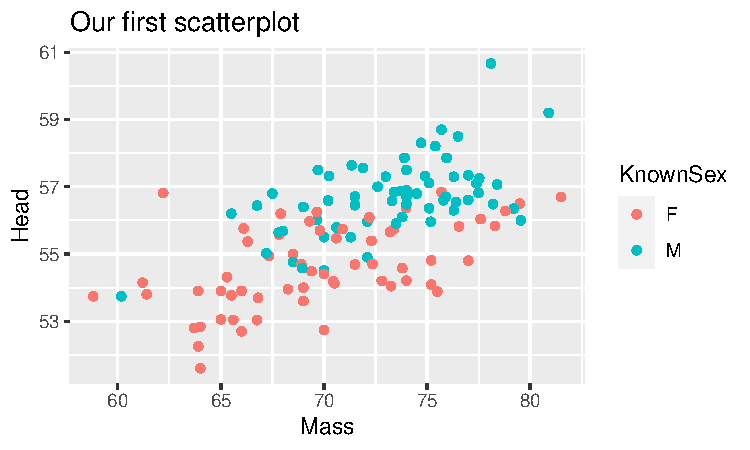
\includegraphics{./intro_files/figure-pdf/unnamed-chunk-11-1.pdf}

}

\end{figure}

The above plot is basically the same as writing:

\begin{Shaded}
\begin{Highlighting}[]
\FunctionTok{ggplot}\NormalTok{(df, }\FunctionTok{aes}\NormalTok{(}\AttributeTok{x=}\NormalTok{Mass, }\AttributeTok{y=}\NormalTok{Head, }\AttributeTok{color =}\NormalTok{ KnownSex) ) }\SpecialCharTok{+} 
  \FunctionTok{geom\_point}\NormalTok{() }\SpecialCharTok{+}
  \FunctionTok{ggtitle}\NormalTok{(}\StringTok{"Our First Scatterplot"}\NormalTok{)}
\end{Highlighting}
\end{Shaded}

\begin{figure}[H]

{\centering \includegraphics{./intro_files/figure-pdf/unnamed-chunk-12-1.pdf}

}

\end{figure}

You'll notice that we are \textbf{chaining} together commands with the
\texttt{+}. This is similar to how we chain together commands with the
\texttt{\%\textgreater{}\%} when doing data carpentry. \texttt{ggplot()}
instead chains with the \texttt{+}. Again, be careful not to start a row
with a \texttt{+}, and you must end a row with a \texttt{+} unless it's
the very last row.

To change the title of the x-axis or the y-axis, we use \texttt{xlab}
and \texttt{ylab} respectively. We can do it like this:

\begin{Shaded}
\begin{Highlighting}[]
\NormalTok{p }\SpecialCharTok{+} \FunctionTok{xlab}\NormalTok{(}\StringTok{"Body Mass (g)"}\NormalTok{) }\SpecialCharTok{+} \FunctionTok{ylab}\NormalTok{(}\StringTok{"Head Size (mm)"}\NormalTok{)}
\end{Highlighting}
\end{Shaded}

\begin{figure}[H]

{\centering \includegraphics{./intro_files/figure-pdf/unnamed-chunk-13-1.pdf}

}

\end{figure}

\hypertarget{colors-shapes-and-sizes}{%
\subsection{Colors, Shapes and Sizes}\label{colors-shapes-and-sizes}}

R recognizes many default color names. These can be found at either of
these places:

\href{https://www.datanovia.com/en/blog/awesome-list-of-657-r-color-names/}{Color
names 1}
\href{http://www.stat.columbia.edu/~tzheng/files/Rcolor.pdf}{Color names
2} Or, you can use a \href{https://htmlcolorcodes.com/color-picker/}{hex
code}

Here we use the color \texttt{dodgerblue} to change all the points to
that color:

\begin{Shaded}
\begin{Highlighting}[]
\FunctionTok{ggplot}\NormalTok{(df, }\FunctionTok{aes}\NormalTok{(}\AttributeTok{x=}\NormalTok{Mass, }\AttributeTok{y=}\NormalTok{Head) ) }\SpecialCharTok{+} \FunctionTok{geom\_point}\NormalTok{(}\AttributeTok{color=}\StringTok{"dodgerblue"}\NormalTok{)}
\end{Highlighting}
\end{Shaded}

\begin{figure}[H]

{\centering \includegraphics{./intro_files/figure-pdf/unnamed-chunk-14-1.pdf}

}

\end{figure}

Here we change the points to the color \texttt{\#ababcc} using a hexcode
- note that hexcodes need to have \texttt{\#} in front of them:

\begin{Shaded}
\begin{Highlighting}[]
\FunctionTok{ggplot}\NormalTok{(df, }\FunctionTok{aes}\NormalTok{(}\AttributeTok{x=}\NormalTok{Mass, }\AttributeTok{y=}\NormalTok{Head) ) }\SpecialCharTok{+} \FunctionTok{geom\_point}\NormalTok{(}\AttributeTok{color=}\StringTok{"\#ababcc"}\NormalTok{)}
\end{Highlighting}
\end{Shaded}

\begin{figure}[H]

{\centering \includegraphics{./intro_files/figure-pdf/unnamed-chunk-15-1.pdf}

}

\end{figure}

You can also change the shape of the points you plot with
\texttt{geom\_point(pch\ =\ )}. You need to insert the appropriate
number according to this guide:

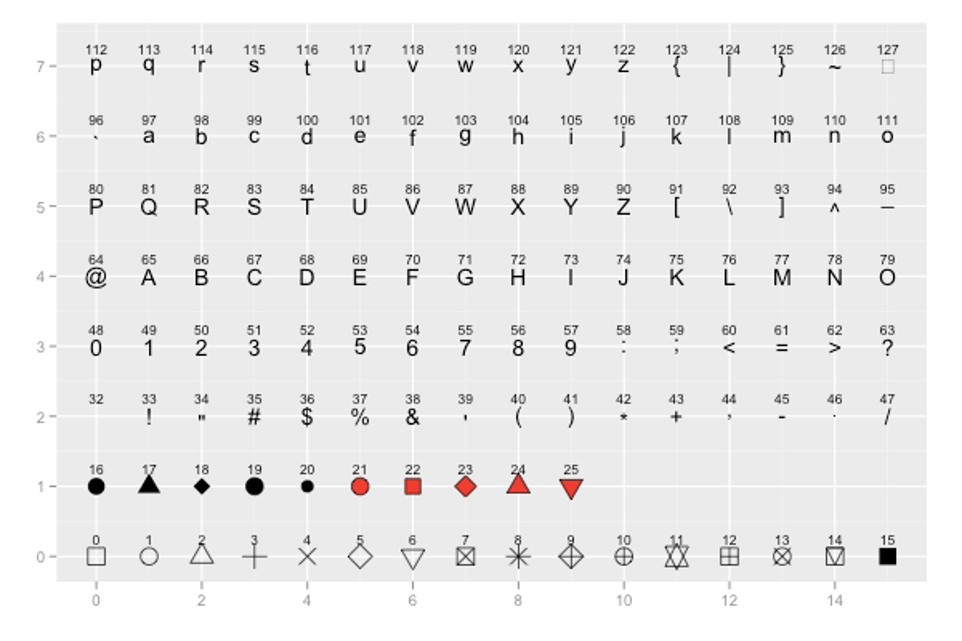
\includegraphics[width=6.25in,height=\textheight]{./img/points.png}

For example, to have dodgerblue asterisks, we add \texttt{pch\ =\ 8},
separating the color and shape commands by a comma:

\begin{Shaded}
\begin{Highlighting}[]
\FunctionTok{ggplot}\NormalTok{(df, }\FunctionTok{aes}\NormalTok{(}\AttributeTok{x=}\NormalTok{Mass, }\AttributeTok{y=}\NormalTok{Head) ) }\SpecialCharTok{+} \FunctionTok{geom\_point}\NormalTok{(}\AttributeTok{color=}\StringTok{"dodgerblue"}\NormalTok{, }\AttributeTok{pch =} \DecValTok{8}\NormalTok{)}
\end{Highlighting}
\end{Shaded}

\begin{figure}[H]

{\centering \includegraphics{./intro_files/figure-pdf/unnamed-chunk-16-1.pdf}

}

\end{figure}

Finally, we can change the size of our datapoints (or other shape we
choose), using \texttt{size\ =}:

\begin{Shaded}
\begin{Highlighting}[]
\FunctionTok{ggplot}\NormalTok{(df, }\FunctionTok{aes}\NormalTok{(}\AttributeTok{x=}\NormalTok{Mass, }\AttributeTok{y=}\NormalTok{Head) ) }\SpecialCharTok{+} \FunctionTok{geom\_point}\NormalTok{(}\AttributeTok{color=}\StringTok{"purple"}\NormalTok{, }\AttributeTok{size=}\DecValTok{2}\NormalTok{)}
\end{Highlighting}
\end{Shaded}

\begin{figure}[H]

{\centering 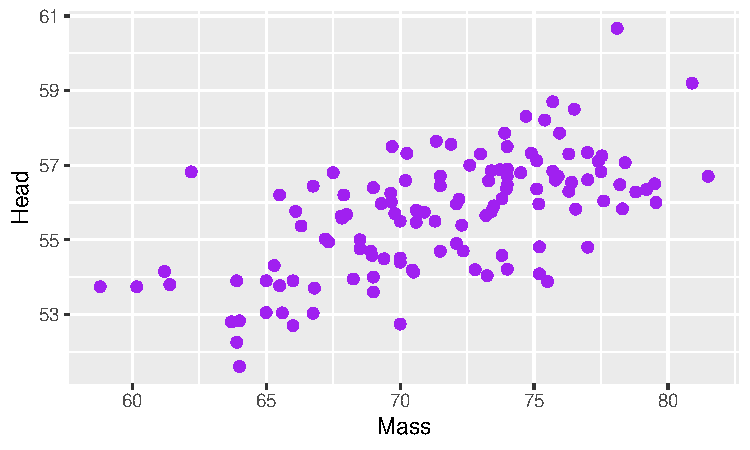
\includegraphics{./intro_files/figure-pdf/unnamed-chunk-17-1.pdf}

}

\end{figure}

\hypertarget{themes}{%
\subsection{Themes}\label{themes}}

\textbf{Default Themes}

You may have noticed that every plot we have made so far has the same
gray background with faint white gridlines. This is the default setting
for the look of \texttt{ggplot()} graphs. There are several other
\texttt{themes} that are available to us that change the overall
appearance of our plots. Some of these are listed below:

\texttt{theme\_bw()} a variation on theme\_grey() that uses a white
background and thin grey grid lines.

\texttt{theme\_linedraw()} A theme with only black lines of various
widths on white backgrounds, reminiscent of a line drawing.

\texttt{theme\_light()} similar to theme\_linedraw() but with light grey
lines and axes, to direct more attention towards the data.

\texttt{theme\_dark()} the dark cousin of theme\_light(), with similar
line sizes but a dark background. Useful to make thin colored lines pop
out.

\texttt{theme\_minimal()} A minimalistic theme with no background
annotations.

\texttt{theme\_classic()} A classic-looking theme, with x and y axis
lines and no gridlines.

\texttt{theme\_void()} A completely empty theme

Let's shows a couple of these different themes. The theme that we use
the most in this course is \texttt{theme\_classic()}. This is how you
would apply this theme to your plot:

\begin{Shaded}
\begin{Highlighting}[]
\FunctionTok{ggplot}\NormalTok{(df, }\FunctionTok{aes}\NormalTok{(}\AttributeTok{x=}\NormalTok{Mass, }\AttributeTok{y=}\NormalTok{Head) ) }\SpecialCharTok{+} 
  \FunctionTok{geom\_point}\NormalTok{() }\SpecialCharTok{+}
  \FunctionTok{theme\_classic}\NormalTok{()}
\end{Highlighting}
\end{Shaded}

\begin{figure}[H]

{\centering 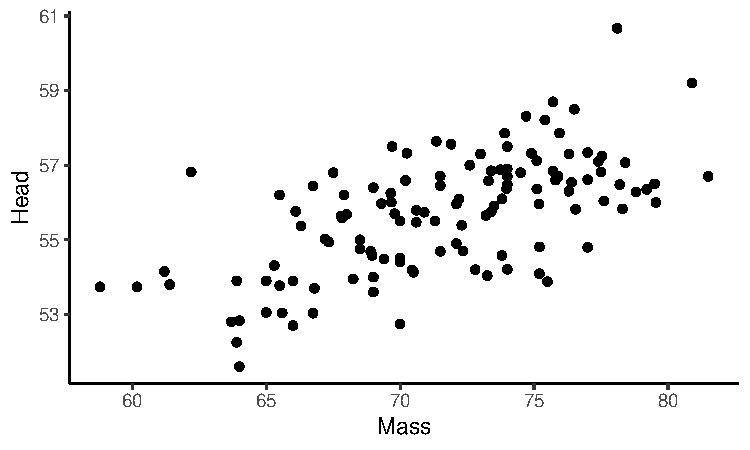
\includegraphics{./intro_files/figure-pdf/unnamed-chunk-18-1.pdf}

}

\end{figure}

It creates a very sleek simple graph. The downside to this type of graph
is that it does get rid of the gridlines which can be helpful sometimes.

Another theme that we use often is \texttt{theme\_minimal()}. Here is
how we would add this:

\begin{Shaded}
\begin{Highlighting}[]
\FunctionTok{ggplot}\NormalTok{(df, }\FunctionTok{aes}\NormalTok{(}\AttributeTok{x=}\NormalTok{Mass, }\AttributeTok{y=}\NormalTok{Head) ) }\SpecialCharTok{+} 
  \FunctionTok{geom\_point}\NormalTok{() }\SpecialCharTok{+}
  \FunctionTok{theme\_minimal}\NormalTok{()}
\end{Highlighting}
\end{Shaded}

\begin{figure}[H]

{\centering 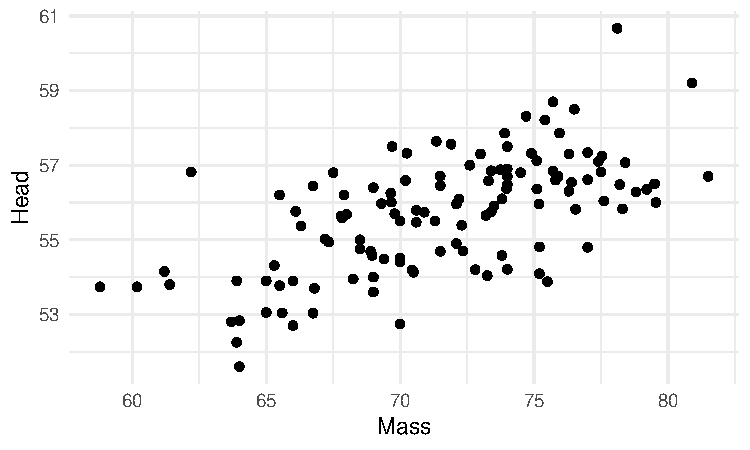
\includegraphics{./intro_files/figure-pdf/unnamed-chunk-19-1.pdf}

}

\end{figure}

This theme is also simplistic, but has gridlines too.

\textbf{Custom themes}

Rather than changing many different aspects of the graph at once, we can
change individual things one by one with \texttt{theme()}. We don't
propose to cover this in more detail in this book - for more information
about themes \href{https://ggplot2-book.org/}{look here} - however, here
is one quick example.

Let's say we wanted to make the panel background light blue instead of
gray. We could do it like this:

\begin{Shaded}
\begin{Highlighting}[]
\FunctionTok{ggplot}\NormalTok{(df, }\FunctionTok{aes}\NormalTok{(}\AttributeTok{x=}\NormalTok{Mass, }\AttributeTok{y=}\NormalTok{Head) ) }\SpecialCharTok{+} 
  \FunctionTok{geom\_point}\NormalTok{() }\SpecialCharTok{+}
  \FunctionTok{theme}\NormalTok{(}\AttributeTok{panel.background =} \FunctionTok{element\_rect}\NormalTok{(}\AttributeTok{fill =} \StringTok{"lightblue"}\NormalTok{))}
\end{Highlighting}
\end{Shaded}

\begin{figure}[H]

{\centering 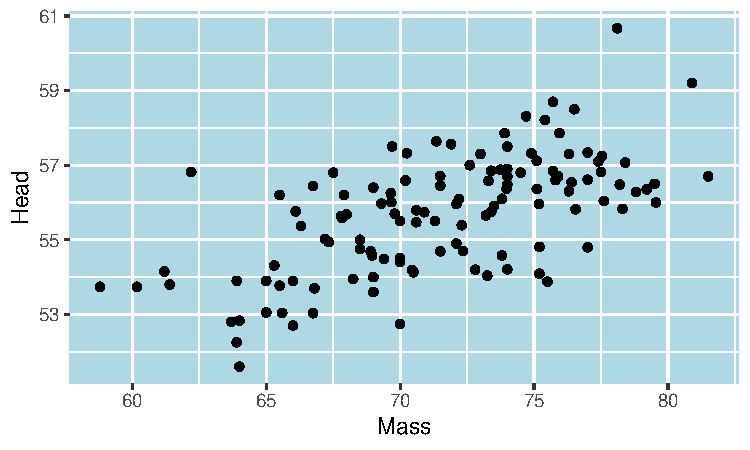
\includegraphics{./intro_files/figure-pdf/unnamed-chunk-20-1.pdf}

}

\end{figure}

Again, this can get quite complicated - so stick with the default themes
if you want to change your plots up a bit, or go to other help guides or
later chapters in this book for more fine detail on customization.

\bookmarksetup{startatroot}

\hypertarget{scatterplots}{%
\chapter{Scatterplots}\label{scatterplots}}

In the introduction to \texttt{ggplot2}, we already demonstrated how to
make a scatterplot. Here we will show a few extra features of these
plots. Scatterplots plot continuous variables on the x- and y-axes, and
can be very useful to examine the association between the two continuous
variables. We use them a lot when plotting data related to correlation.

\hypertarget{basic-scatterplots}{%
\section{Basic Scatterplots}\label{basic-scatterplots}}

As we showed earlier, \texttt{geom\_point} is used to add datapoints to
scatter plots. We'll do this for the \texttt{cheese.csv} dataset, that
contains nutritional information about various cheeses:

\begin{Shaded}
\begin{Highlighting}[]
\FunctionTok{library}\NormalTok{(tidyverse)}
\NormalTok{cheese }\OtherTok{\textless{}{-}} \FunctionTok{read\_csv}\NormalTok{(}\StringTok{"data\_raw/cheese.csv"}\NormalTok{)}
\FunctionTok{head}\NormalTok{(cheese)}
\end{Highlighting}
\end{Shaded}

\begin{verbatim}
# A tibble: 6 x 9
  type      sat_fat polysat_fat monosat_fat protein  carb  chol fiber  kcal
  <chr>       <dbl>       <dbl>       <dbl>   <dbl> <dbl> <dbl> <dbl> <dbl>
1 blue         18.7       0.8          7.78    21.4  2.34    75     0   353
2 brick        18.8       0.784        8.60    23.2  2.79    94     0   371
3 brie         17.4       0.826        8.01    20.8  0.45   100     0   334
4 camembert    15.3       0.724        7.02    19.8  0.46    72     0   300
5 caraway      18.6       0.83         8.28    25.2  3.06    93     0   376
6 cheddar      21.1       0.942        9.39    24.9  1.28   105     0   403
\end{verbatim}

We'll start with a simple scatterplot looking at the association between
saturated fat on the x-axis and cholesterol on the y-axis intake.

\begin{Shaded}
\begin{Highlighting}[]
\FunctionTok{ggplot}\NormalTok{(cheese, }\FunctionTok{aes}\NormalTok{(}\AttributeTok{x=}\NormalTok{sat\_fat, }\AttributeTok{y=}\NormalTok{chol) ) }\SpecialCharTok{+} 
  \FunctionTok{geom\_point}\NormalTok{()}
\end{Highlighting}
\end{Shaded}

\begin{figure}[H]

{\centering 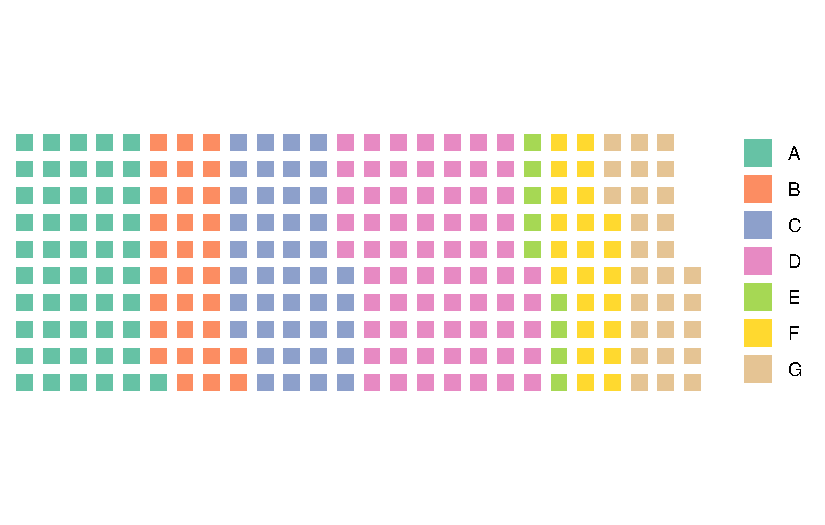
\includegraphics{./scatterplots_files/figure-pdf/unnamed-chunk-2-1.pdf}

}

\end{figure}

We can change the color of the points by adding a color inside of
\texttt{geom\_point} - making sure that the color name is in quotes:

\begin{Shaded}
\begin{Highlighting}[]
\FunctionTok{ggplot}\NormalTok{(cheese, }\FunctionTok{aes}\NormalTok{(}\AttributeTok{x=}\NormalTok{sat\_fat, }\AttributeTok{y=}\NormalTok{chol) ) }\SpecialCharTok{+} 
  \FunctionTok{geom\_point}\NormalTok{(}\AttributeTok{color =} \StringTok{"purple"}\NormalTok{)}
\end{Highlighting}
\end{Shaded}

\begin{figure}[H]

{\centering \includegraphics{./scatterplots_files/figure-pdf/unnamed-chunk-3-1.pdf}

}

\end{figure}

To add a straight trendline through the data we use
\texttt{+\ stat\_smooth(method\ =\ "lm")}. The \texttt{stat\_smooth} bit
tells it to add a trendline, and the \texttt{method="lm"} bit in the
middle is telling it to make the straight line:

\begin{Shaded}
\begin{Highlighting}[]
\FunctionTok{ggplot}\NormalTok{(cheese, }\FunctionTok{aes}\NormalTok{(}\AttributeTok{x=}\NormalTok{sat\_fat, }\AttributeTok{y=}\NormalTok{chol) ) }\SpecialCharTok{+} 
  \FunctionTok{geom\_point}\NormalTok{(}\AttributeTok{color =} \StringTok{"purple"}\NormalTok{) }\SpecialCharTok{+}
 \FunctionTok{stat\_smooth}\NormalTok{(}\AttributeTok{method =} \StringTok{"lm"}\NormalTok{)}
\end{Highlighting}
\end{Shaded}

\begin{figure}[H]

{\centering \includegraphics{./scatterplots_files/figure-pdf/unnamed-chunk-4-1.pdf}

}

\end{figure}

Here you can see it automatically puts a shaded area around your
trendline, which represents a confidence interval around the trendline.
There is a way to remove it by adding \texttt{se\ =\ FALSE} or
\texttt{se\ =\ F} inside of \texttt{stat\_smooth()}:

\begin{Shaded}
\begin{Highlighting}[]
\FunctionTok{ggplot}\NormalTok{(cheese, }\FunctionTok{aes}\NormalTok{(}\AttributeTok{x=}\NormalTok{sat\_fat, }\AttributeTok{y=}\NormalTok{chol) ) }\SpecialCharTok{+} 
  \FunctionTok{geom\_point}\NormalTok{(}\AttributeTok{color =} \StringTok{"purple"}\NormalTok{) }\SpecialCharTok{+}
 \FunctionTok{stat\_smooth}\NormalTok{(}\AttributeTok{method =} \StringTok{"lm"}\NormalTok{, }\AttributeTok{se =} \ConstantTok{FALSE}\NormalTok{)}
\end{Highlighting}
\end{Shaded}

\begin{figure}[H]

{\centering \includegraphics{./scatterplots_files/figure-pdf/unnamed-chunk-5-1.pdf}

}

\end{figure}

You can also change the color of the trendline, by adding to
\texttt{stat\_smooth}

\begin{Shaded}
\begin{Highlighting}[]
\FunctionTok{ggplot}\NormalTok{(cheese, }\FunctionTok{aes}\NormalTok{(}\AttributeTok{x=}\NormalTok{sat\_fat, }\AttributeTok{y=}\NormalTok{chol) ) }\SpecialCharTok{+} 
  \FunctionTok{geom\_point}\NormalTok{(}\AttributeTok{color =} \StringTok{"purple"}\NormalTok{) }\SpecialCharTok{+}
  \FunctionTok{stat\_smooth}\NormalTok{(}\AttributeTok{method =} \StringTok{"lm"}\NormalTok{, }\AttributeTok{se=}\NormalTok{ F, }\AttributeTok{color =} \StringTok{"black"}\NormalTok{)}
\end{Highlighting}
\end{Shaded}

\begin{figure}[H]

{\centering \includegraphics{./scatterplots_files/figure-pdf/unnamed-chunk-6-1.pdf}

}

\end{figure}

As with all \texttt{ggplot2} graphs, you can customize the plot. For
example changing the theme, adding a title and axes titles:

\begin{Shaded}
\begin{Highlighting}[]
\FunctionTok{ggplot}\NormalTok{(cheese, }\FunctionTok{aes}\NormalTok{(}\AttributeTok{x=}\NormalTok{sat\_fat, }\AttributeTok{y=}\NormalTok{chol) ) }\SpecialCharTok{+} 
  \FunctionTok{geom\_point}\NormalTok{(}\AttributeTok{color =} \StringTok{"purple"}\NormalTok{) }\SpecialCharTok{+}
  \FunctionTok{stat\_smooth}\NormalTok{(}\AttributeTok{method =} \StringTok{"lm"}\NormalTok{, }\AttributeTok{se=}\NormalTok{ F, }\AttributeTok{color =} \StringTok{"black"}\NormalTok{) }\SpecialCharTok{+}
  \FunctionTok{xlab}\NormalTok{(}\StringTok{" Saturated Fat"}\NormalTok{) }\SpecialCharTok{+}
  \FunctionTok{ylab}\NormalTok{(}\StringTok{"Cholesterol"}\NormalTok{) }\SpecialCharTok{+}
  \FunctionTok{ggtitle}\NormalTok{(}\StringTok{"Saturated Fat vs Cholesterol"}\NormalTok{) }\SpecialCharTok{+}
  \FunctionTok{theme\_minimal}\NormalTok{()}
\end{Highlighting}
\end{Shaded}

\begin{figure}[H]

{\centering \includegraphics{./scatterplots_files/figure-pdf/unnamed-chunk-7-1.pdf}

}

\end{figure}

If you wish to change the color of the points based on a grouping
variable, then we need to put our \texttt{color=} into the
\texttt{aes()}. You then need to provide the column that has the color
grouping variable. For example, to change the color of points in our
plot of body mass against head size in Blue Jays based on the sex of
birds:

\begin{Shaded}
\begin{Highlighting}[]
\NormalTok{df }\OtherTok{\textless{}{-}} \FunctionTok{read\_csv}\NormalTok{(}\StringTok{"data\_raw/BlueJays.csv"}\NormalTok{)}
\end{Highlighting}
\end{Shaded}

\begin{verbatim}
Rows: 123 Columns: 9
-- Column specification --------------------------------------------------------
Delimiter: ","
chr (2): BirdID, KnownSex
dbl (7): BillDepth, BillWidth, BillLength, Head, Mass, Skull, Sex

i Use `spec()` to retrieve the full column specification for this data.
i Specify the column types or set `show_col_types = FALSE` to quiet this message.
\end{verbatim}

\begin{Shaded}
\begin{Highlighting}[]
\FunctionTok{head}\NormalTok{(df)}
\end{Highlighting}
\end{Shaded}

\begin{verbatim}
# A tibble: 6 x 9
  BirdID     KnownSex BillDepth BillWidth BillLength  Head  Mass Skull   Sex
  <chr>      <chr>        <dbl>     <dbl>      <dbl> <dbl> <dbl> <dbl> <dbl>
1 0000-00000 M             8.26      9.21       25.9  56.6  73.3  30.7     1
2 1142-05901 M             8.54      8.76       25.0  56.4  75.1  31.4     1
3 1142-05905 M             8.39      8.78       26.1  57.3  70.2  31.2     1
4 1142-05907 F             7.78      9.3        23.5  53.8  65.5  30.3     0
5 1142-05909 M             8.71      9.84       25.5  57.3  74.9  31.8     1
6 1142-05911 F             7.28      9.3        22.2  52.2  63.9  30       0
\end{verbatim}

\begin{Shaded}
\begin{Highlighting}[]
\FunctionTok{ggplot}\NormalTok{(df, }\FunctionTok{aes}\NormalTok{(}\AttributeTok{x=}\NormalTok{Mass, }\AttributeTok{y=}\NormalTok{Head, }\AttributeTok{color =}\NormalTok{ KnownSex) ) }\SpecialCharTok{+} 
  \FunctionTok{geom\_point}\NormalTok{() }
\end{Highlighting}
\end{Shaded}

\begin{figure}[H]

{\centering \includegraphics{./scatterplots_files/figure-pdf/unnamed-chunk-8-1.pdf}

}

\end{figure}

If you wish to customize the colors of your datapoints, then you need to
add \texttt{scale\_color\_manual()} like this:

\begin{Shaded}
\begin{Highlighting}[]
\FunctionTok{ggplot}\NormalTok{(df, }\FunctionTok{aes}\NormalTok{(}\AttributeTok{x=}\NormalTok{Mass, }\AttributeTok{y=}\NormalTok{Head, }\AttributeTok{color =}\NormalTok{ KnownSex) ) }\SpecialCharTok{+} 
  \FunctionTok{geom\_point}\NormalTok{() }\SpecialCharTok{+}
  \FunctionTok{scale\_color\_manual}\NormalTok{(}\AttributeTok{values =} \FunctionTok{c}\NormalTok{(}\StringTok{"darkorange"}\NormalTok{, }\StringTok{"steelblue2"}\NormalTok{)) }\SpecialCharTok{+}
  \FunctionTok{theme\_classic}\NormalTok{()}
\end{Highlighting}
\end{Shaded}

\begin{figure}[H]

{\centering \includegraphics{./scatterplots_files/figure-pdf/unnamed-chunk-9-1.pdf}

}

\end{figure}

If you have a lot of points on your scatterplot, it can get quite hard
to see all the datapoints. One way to deal with this is to change the
\textbf{transparency} of the points. You can do this by adjusting the
\texttt{alpha} level inside of \texttt{geom\_point()}. \texttt{alpha=}
ranges from 0 to 1, with 0 being fully transparent and 1 being fully
solid.

\begin{Shaded}
\begin{Highlighting}[]
\FunctionTok{ggplot}\NormalTok{(df, }\FunctionTok{aes}\NormalTok{(}\AttributeTok{x=}\NormalTok{Mass, }\AttributeTok{y=}\NormalTok{Head, }\AttributeTok{color =}\NormalTok{ KnownSex) ) }\SpecialCharTok{+} 
  \FunctionTok{geom\_point}\NormalTok{(}\AttributeTok{alpha=}\NormalTok{.}\DecValTok{4}\NormalTok{) }\SpecialCharTok{+}
  \FunctionTok{scale\_color\_manual}\NormalTok{(}\AttributeTok{values =} \FunctionTok{c}\NormalTok{(}\StringTok{"darkorange"}\NormalTok{, }\StringTok{"steelblue2"}\NormalTok{)) }\SpecialCharTok{+}
  \FunctionTok{theme\_classic}\NormalTok{()}
\end{Highlighting}
\end{Shaded}

\begin{figure}[H]

{\centering \includegraphics{./scatterplots_files/figure-pdf/unnamed-chunk-10-1.pdf}

}

\end{figure}

\hypertarget{multiple-groups-on-a-scatterplot}{%
\section{Multiple Groups on a
Scatterplot}\label{multiple-groups-on-a-scatterplot}}

We can add multiple trendlines to each group of datapoints plotted on a
scatterplot. Let's look at the following data of the chemical components
of different olive oils produced in Italy. This is what the data look
like:

\begin{Shaded}
\begin{Highlighting}[]
\NormalTok{olives }\OtherTok{\textless{}{-}} \FunctionTok{read\_csv}\NormalTok{(}\StringTok{"data\_raw/olives.csv"}\NormalTok{)}
\FunctionTok{head}\NormalTok{(olives)}
\end{Highlighting}
\end{Shaded}

\begin{verbatim}
# A tibble: 6 x 10
  macro.a~1 region palmi~2 palmi~3 stearic oleic linol~4 linol~5 arach~6 eicos~7
  <chr>     <chr>    <dbl>   <dbl>   <dbl> <dbl>   <dbl>   <dbl>   <dbl>   <dbl>
1 South     Apuli~    1075      75     226  7823     672      36      60      29
2 South     Apuli~    1088      73     224  7709     781      31      61      29
3 South     Apuli~     911      54     246  8113     549      31      63      29
4 South     Apuli~     966      57     240  7952     619      50      78      35
5 South     Apuli~    1051      67     259  7771     672      50      80      46
6 South     Apuli~     911      49     268  7924     678      51      70      44
# ... with abbreviated variable names 1: macro.area, 2: palmitic,
#   3: palmitoleic, 4: linoleic, 5: linolenic, 6: arachidic, 7: eicosenoic
\end{verbatim}

If we use \texttt{table()}, we can see how many different regions are
represented in the data. There are three unique Italian areas where the
olives come from:

\begin{Shaded}
\begin{Highlighting}[]
\FunctionTok{table}\NormalTok{(olives}\SpecialCharTok{$}\NormalTok{macro.area)}
\end{Highlighting}
\end{Shaded}

\begin{verbatim}

Centre.North     Sardinia        South 
         151           98          323 
\end{verbatim}

Say we are interested in looking at how \texttt{oleic} and
\texttt{linoleic} acid contents are related to each other by
\texttt{macro.area}:

\begin{Shaded}
\begin{Highlighting}[]
\FunctionTok{ggplot}\NormalTok{(olives, }\FunctionTok{aes}\NormalTok{(}\AttributeTok{x=}\NormalTok{oleic, }\AttributeTok{y=}\NormalTok{linoleic, }\AttributeTok{color=}\NormalTok{macro.area)) }\SpecialCharTok{+}
  \FunctionTok{geom\_point}\NormalTok{() }\SpecialCharTok{+}
  \FunctionTok{theme\_classic}\NormalTok{()}
\end{Highlighting}
\end{Shaded}

\begin{figure}[H]

{\centering \includegraphics{./scatterplots_files/figure-pdf/unnamed-chunk-13-1.pdf}

}

\end{figure}

If we wanted to add a trendline for each area, all we need to do is add
our \texttt{stat\_smooth(method="lm)} line to the code. It already knows
to plot these as separate trendlines for each group because inside
\texttt{aes()} we have \texttt{color=macro.area}. As long as there is a
\texttt{group=} or \texttt{color=} inside \texttt{aes()} then it knows
to do things like adding trendlines separately for each group:

\begin{Shaded}
\begin{Highlighting}[]
\FunctionTok{ggplot}\NormalTok{(olives, }\FunctionTok{aes}\NormalTok{(}\AttributeTok{x=}\NormalTok{oleic, }\AttributeTok{y=}\NormalTok{linoleic, }\AttributeTok{color=}\NormalTok{macro.area)) }\SpecialCharTok{+}
  \FunctionTok{geom\_point}\NormalTok{() }\SpecialCharTok{+}
  \FunctionTok{stat\_smooth}\NormalTok{(}\AttributeTok{method=}\StringTok{"lm"}\NormalTok{, }\AttributeTok{se=}\NormalTok{F) }\SpecialCharTok{+}
  \FunctionTok{theme\_classic}\NormalTok{() }
\end{Highlighting}
\end{Shaded}

\begin{figure}[H]

{\centering \includegraphics{./scatterplots_files/figure-pdf/unnamed-chunk-14-1.pdf}

}

\end{figure}

\hypertarget{bubble-charts}{%
\section{Bubble Charts}\label{bubble-charts}}

Bubble Charts are an extension to scatterplots. In scatterplots we plot
two continuous variables against each other. With a bubble chart we add
a third continuous variable and vary the size of our datapoints
according to this variable. For example, say we wish to also plot skull
size on our Blue Jay scatterplot. We could increase the size of the
points for individuals with larger skull sizes. We do this by adding
\texttt{size=Skull} into our \texttt{aes()} part:

\begin{Shaded}
\begin{Highlighting}[]
\FunctionTok{ggplot}\NormalTok{(df, }\FunctionTok{aes}\NormalTok{(}\AttributeTok{x=}\NormalTok{Mass, }\AttributeTok{y=}\NormalTok{Head, }\AttributeTok{color =}\NormalTok{ KnownSex, }\AttributeTok{size =}\NormalTok{ Skull) ) }\SpecialCharTok{+} 
  \FunctionTok{geom\_point}\NormalTok{(}\AttributeTok{alpha=}\NormalTok{.}\DecValTok{4}\NormalTok{) }\SpecialCharTok{+}
  \FunctionTok{scale\_color\_manual}\NormalTok{(}\AttributeTok{values =} \FunctionTok{c}\NormalTok{(}\StringTok{"darkorange"}\NormalTok{, }\StringTok{"steelblue2"}\NormalTok{)) }\SpecialCharTok{+}
  \FunctionTok{theme\_classic}\NormalTok{()}
\end{Highlighting}
\end{Shaded}

\begin{figure}[H]

{\centering \includegraphics{./scatterplots_files/figure-pdf/unnamed-chunk-15-1.pdf}

}

\end{figure}

The issue with bubble charts is that they can start to look very
cluttered, making it hard to actually see any patterns. They should
probably be used sparingly. One trick you can employ to make them a
little easier to see is to add \texttt{scale\_size()} to the plot. Here,
you enter two numbers to tell it what size points to scale to. In our
example below, we used \texttt{scale\_size(range\ =\ c(.1,\ 4))} which
makes our points range between sizes 0.1 and 4. This makes the plot a
little less busy:

\begin{Shaded}
\begin{Highlighting}[]
\FunctionTok{ggplot}\NormalTok{(df, }\FunctionTok{aes}\NormalTok{(}\AttributeTok{x=}\NormalTok{Mass, }\AttributeTok{y=}\NormalTok{Head, }\AttributeTok{color =}\NormalTok{ KnownSex, }\AttributeTok{size =}\NormalTok{ Skull) ) }\SpecialCharTok{+} 
  \FunctionTok{geom\_point}\NormalTok{(}\AttributeTok{alpha=}\NormalTok{.}\DecValTok{4}\NormalTok{) }\SpecialCharTok{+}
  \FunctionTok{scale\_color\_manual}\NormalTok{(}\AttributeTok{values =} \FunctionTok{c}\NormalTok{(}\StringTok{"darkorange"}\NormalTok{, }\StringTok{"steelblue2"}\NormalTok{)) }\SpecialCharTok{+}
  \FunctionTok{theme\_classic}\NormalTok{() }\SpecialCharTok{+}
  \FunctionTok{scale\_size}\NormalTok{(}\AttributeTok{range =} \FunctionTok{c}\NormalTok{(.}\DecValTok{1}\NormalTok{, }\DecValTok{4}\NormalTok{))}
\end{Highlighting}
\end{Shaded}

\begin{figure}[H]

{\centering \includegraphics{./scatterplots_files/figure-pdf/unnamed-chunk-16-1.pdf}

}

\end{figure}

\bookmarksetup{startatroot}

\hypertarget{line-graphs}{%
\chapter{Line Graphs}\label{line-graphs}}

Line graphs connect continuous values on the y-axis over time on the
x-axis. They are very useful for show patterns of change over time.

\hypertarget{basic-line-graphs}{%
\section{Basic Line Graphs}\label{basic-line-graphs}}

Let's look at the \texttt{jennifer.csv} dataset:

\begin{Shaded}
\begin{Highlighting}[]
\FunctionTok{library}\NormalTok{(tidyverse)}
\NormalTok{jennifer }\OtherTok{\textless{}{-}} \FunctionTok{read\_csv}\NormalTok{(}\StringTok{"data\_raw/jennifer.csv"}\NormalTok{)}
\FunctionTok{head}\NormalTok{(jennifer)}
\end{Highlighting}
\end{Shaded}

\begin{verbatim}
# A tibble: 6 x 5
   year sex    name         n       prop
  <dbl> <chr>  <chr>    <dbl>      <dbl>
1  1916 Female Jennifer     5 0.00000461
2  1919 Female Jennifer     6 0.00000511
3  1920 Female Jennifer     7 0.00000563
4  1921 Female Jennifer     5 0.00000391
5  1922 Female Jennifer     7 0.00000561
6  1923 Female Jennifer     9 0.00000719
\end{verbatim}

This dataset shows the number \texttt{n} of children born each year
(\texttt{year}) in the United States with the name Jennifer. In 1916
there were five children born with the name Jennifer. In 1917 there were
0. In 1923 there were 9.

This dataset goes up to 2017 where there were 1052 children born with
the name Jennifer:

\begin{Shaded}
\begin{Highlighting}[]
\FunctionTok{tail}\NormalTok{(jennifer)}
\end{Highlighting}
\end{Shaded}

\begin{verbatim}
# A tibble: 6 x 5
   year sex    name         n     prop
  <dbl> <chr>  <chr>    <dbl>    <dbl>
1  2012 Female Jennifer  1923 0.000993
2  2013 Female Jennifer  1689 0.000878
3  2014 Female Jennifer  1521 0.000779
4  2015 Female Jennifer  1283 0.000660
5  2016 Female Jennifer  1159 0.000601
6  2017 Female Jennifer  1042 0.000556
\end{verbatim}

Therefore, we have a continuous variable (\texttt{n}) and a time
variable (\texttt{year}). We can plot these as we would plot a
scatterplot by supplying \texttt{year} to our x-axis and \texttt{n} to
our y-axis. We could then add datapoints with \texttt{geom\_point()}
essentially making a scatterplot:

\begin{Shaded}
\begin{Highlighting}[]
\FunctionTok{ggplot}\NormalTok{(jennifer, }\FunctionTok{aes}\NormalTok{(}\AttributeTok{x=}\NormalTok{year, }\AttributeTok{y=}\NormalTok{n) ) }\SpecialCharTok{+} \FunctionTok{geom\_point}\NormalTok{() }
\end{Highlighting}
\end{Shaded}

\begin{figure}[H]

{\centering \includegraphics{./lines_files/figure-pdf/unnamed-chunk-3-1.pdf}

}

\end{figure}

But, we aren't dealing with just a scatterplot. These datapoints can be
connected to each other as they are ordered in time. Instead of using
\texttt{geom\_point()} we can use \texttt{geom\_line()} to draw a line
instead:

\begin{Shaded}
\begin{Highlighting}[]
\FunctionTok{ggplot}\NormalTok{(jennifer, }\FunctionTok{aes}\NormalTok{(}\AttributeTok{x=}\NormalTok{year, }\AttributeTok{y=}\NormalTok{n) ) }\SpecialCharTok{+} \FunctionTok{geom\_line}\NormalTok{()}
\end{Highlighting}
\end{Shaded}

\begin{figure}[H]

{\centering \includegraphics{./lines_files/figure-pdf/unnamed-chunk-4-1.pdf}

}

\end{figure}

If you so desired, you could plot both the points and lines together:

\begin{Shaded}
\begin{Highlighting}[]
\FunctionTok{ggplot}\NormalTok{(jennifer, }\FunctionTok{aes}\NormalTok{(}\AttributeTok{x=}\NormalTok{year, }\AttributeTok{y=}\NormalTok{n) ) }\SpecialCharTok{+} 
  \FunctionTok{geom\_point}\NormalTok{() }\SpecialCharTok{+}  
  \FunctionTok{geom\_line}\NormalTok{() }
\end{Highlighting}
\end{Shaded}

\begin{figure}[H]

{\centering \includegraphics{./lines_files/figure-pdf/unnamed-chunk-5-1.pdf}

}

\end{figure}

You can adjust the colors of the lines and the points independently by
supplying \texttt{color=} inside of each geom:

e.g.~Changing the color of the line, but \emph{not} the points:

\begin{Shaded}
\begin{Highlighting}[]
\FunctionTok{ggplot}\NormalTok{(jennifer, }\FunctionTok{aes}\NormalTok{(}\AttributeTok{x=}\NormalTok{year, }\AttributeTok{y=}\NormalTok{n) ) }\SpecialCharTok{+} 
  \FunctionTok{geom\_point}\NormalTok{() }\SpecialCharTok{+}
  \FunctionTok{geom\_line}\NormalTok{(}\AttributeTok{color =} \StringTok{"purple"}\NormalTok{) }
\end{Highlighting}
\end{Shaded}

\begin{figure}[H]

{\centering \includegraphics{./lines_files/figure-pdf/unnamed-chunk-6-1.pdf}

}

\end{figure}

Changing the color of both the points and the line:

\begin{Shaded}
\begin{Highlighting}[]
\FunctionTok{ggplot}\NormalTok{(jennifer, }\FunctionTok{aes}\NormalTok{(}\AttributeTok{x=}\NormalTok{year, }\AttributeTok{y=}\NormalTok{n) ) }\SpecialCharTok{+} 
  \FunctionTok{geom\_point}\NormalTok{(}\AttributeTok{color =} \StringTok{"violet"}\NormalTok{) }\SpecialCharTok{+}
  \FunctionTok{geom\_line}\NormalTok{(}\AttributeTok{color =} \StringTok{"purple"}\NormalTok{) }
\end{Highlighting}
\end{Shaded}

\begin{figure}[H]

{\centering \includegraphics{./lines_files/figure-pdf/unnamed-chunk-7-1.pdf}

}

\end{figure}

You can also change the width of lines by adding \texttt{lwd=} to
\texttt{geom\_line()}:

\begin{Shaded}
\begin{Highlighting}[]
\FunctionTok{ggplot}\NormalTok{(jennifer, }\FunctionTok{aes}\NormalTok{(}\AttributeTok{x=}\NormalTok{year, }\AttributeTok{y=}\NormalTok{n) ) }\SpecialCharTok{+} 
  \FunctionTok{geom\_line}\NormalTok{(}\AttributeTok{color =} \StringTok{"purple"}\NormalTok{, }\AttributeTok{lwd=}\DecValTok{2}\NormalTok{)}
\end{Highlighting}
\end{Shaded}

\begin{figure}[H]

{\centering \includegraphics{./lines_files/figure-pdf/unnamed-chunk-8-1.pdf}

}

\end{figure}

There are also several different styles of lines. You can change these
by adjusting the number you provide to \texttt{lty=} inside of
\texttt{geom\_line()}. Here are a few examples:

\begin{Shaded}
\begin{Highlighting}[]
\FunctionTok{ggplot}\NormalTok{(jennifer, }\FunctionTok{aes}\NormalTok{(}\AttributeTok{x=}\NormalTok{year, }\AttributeTok{y=}\NormalTok{n) ) }\SpecialCharTok{+} \FunctionTok{geom\_line}\NormalTok{(}\AttributeTok{lty=}\DecValTok{2}\NormalTok{)}
\end{Highlighting}
\end{Shaded}

\begin{figure}[H]

{\centering \includegraphics{./lines_files/figure-pdf/unnamed-chunk-9-1.pdf}

}

\end{figure}

\begin{Shaded}
\begin{Highlighting}[]
\FunctionTok{ggplot}\NormalTok{(jennifer, }\FunctionTok{aes}\NormalTok{(}\AttributeTok{x=}\NormalTok{year, }\AttributeTok{y=}\NormalTok{n) ) }\SpecialCharTok{+} \FunctionTok{geom\_line}\NormalTok{(}\AttributeTok{lty=}\DecValTok{3}\NormalTok{)}
\end{Highlighting}
\end{Shaded}

\begin{figure}[H]

{\centering \includegraphics{./lines_files/figure-pdf/unnamed-chunk-10-1.pdf}

}

\end{figure}

This illustration shows some of the linetype options:

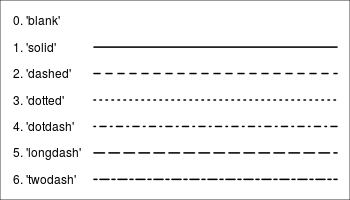
\includegraphics{./img/lty.png}

Just a quick reminder: Please only connect datapoints into a line if it
is meaningful to do so! This is almost always when your x-axis is some
measure of time.

\hypertarget{multiple-line-graphs}{%
\section{Multiple Line Graphs}\label{multiple-line-graphs}}

Often we wish to compare the patterns over time of different groups. We
can do that by plotting \emph{multiple} lines on the same graph.

Let's look at this example dataset.

\begin{Shaded}
\begin{Highlighting}[]
\NormalTok{jenlinda }\OtherTok{\textless{}{-}} \FunctionTok{read\_csv}\NormalTok{(}\StringTok{"data\_raw/jenlinda.csv"}\NormalTok{)}
\FunctionTok{tail}\NormalTok{(jenlinda)}
\end{Highlighting}
\end{Shaded}

\begin{verbatim}
# A tibble: 6 x 5
   year sex    name         n     prop
  <dbl> <chr>  <chr>    <dbl>    <dbl>
1  2015 Female Jennifer  1283 0.000660
2  2015 Female Linda      425 0.000218
3  2016 Female Jennifer  1159 0.000601
4  2016 Female Linda      436 0.000226
5  2017 Female Jennifer  1042 0.000556
6  2017 Female Linda      404 0.000215
\end{verbatim}

Here, we have data in \textbf{long} format. We still have our continuous
outcome variable of \texttt{n} in one column. We also have \texttt{year}
in another column. So we can plot these two against each other.
Importantly, we can split our lines based on our grouping variable,
which is the \texttt{name} column. In that column we have two different
groups - Jennifer and Linda.

To plot separate lines based on the \texttt{name} column, we need to add
\texttt{group=name} to our \texttt{aes()}. We've also added some custom
labels, titles and a theme.

\begin{Shaded}
\begin{Highlighting}[]
\FunctionTok{ggplot}\NormalTok{(jenlinda, }\FunctionTok{aes}\NormalTok{(}\AttributeTok{x=}\NormalTok{year, }\AttributeTok{y=}\NormalTok{n, }\AttributeTok{group=}\NormalTok{name)) }\SpecialCharTok{+} 
  \FunctionTok{geom\_line}\NormalTok{()}\SpecialCharTok{+}
  \FunctionTok{xlab}\NormalTok{(}\StringTok{"Year"}\NormalTok{) }\SpecialCharTok{+}
  \FunctionTok{ylab}\NormalTok{(}\StringTok{"Number of Children Born"}\NormalTok{) }\SpecialCharTok{+}
  \FunctionTok{ggtitle}\NormalTok{(}\StringTok{"Popularity of Names Jennifer \& Linda in USA"}\NormalTok{) }\SpecialCharTok{+}
  \FunctionTok{theme\_minimal}\NormalTok{()}
\end{Highlighting}
\end{Shaded}

\begin{figure}[H]

{\centering \includegraphics{./lines_files/figure-pdf/unnamed-chunk-12-1.pdf}

}

\end{figure}

You may notice that both lines are the same color! To make the lines
have different colors, we insert \texttt{color=name} into the
\texttt{aes()} instead of \texttt{group=name}:

\begin{Shaded}
\begin{Highlighting}[]
\FunctionTok{ggplot}\NormalTok{(jenlinda, }\FunctionTok{aes}\NormalTok{(}\AttributeTok{x=}\NormalTok{year, }\AttributeTok{y=}\NormalTok{n, }\AttributeTok{color=}\NormalTok{name)) }\SpecialCharTok{+} 
  \FunctionTok{geom\_line}\NormalTok{()}\SpecialCharTok{+}
  \FunctionTok{xlab}\NormalTok{(}\StringTok{"Year"}\NormalTok{) }\SpecialCharTok{+}
  \FunctionTok{ylab}\NormalTok{(}\StringTok{"Number of Children Born"}\NormalTok{) }\SpecialCharTok{+}
  \FunctionTok{ggtitle}\NormalTok{(}\StringTok{"Popularity of Names Jennifer \& Linda in USA"}\NormalTok{) }\SpecialCharTok{+}
  \FunctionTok{theme\_minimal}\NormalTok{()}
\end{Highlighting}
\end{Shaded}

\begin{figure}[H]

{\centering \includegraphics{./lines_files/figure-pdf/unnamed-chunk-13-1.pdf}

}

\end{figure}

Again, we could customize these colors if we did not like them with
\texttt{scale\_color\_manual()} like this:

\begin{Shaded}
\begin{Highlighting}[]
\FunctionTok{ggplot}\NormalTok{(jenlinda, }\FunctionTok{aes}\NormalTok{(}\AttributeTok{x=}\NormalTok{year, }\AttributeTok{y=}\NormalTok{n, }\AttributeTok{color=}\NormalTok{name)) }\SpecialCharTok{+} 
  \FunctionTok{geom\_line}\NormalTok{()}\SpecialCharTok{+}
  \FunctionTok{xlab}\NormalTok{(}\StringTok{"Year"}\NormalTok{) }\SpecialCharTok{+}
  \FunctionTok{ylab}\NormalTok{(}\StringTok{"Number of Children Born"}\NormalTok{) }\SpecialCharTok{+}
  \FunctionTok{ggtitle}\NormalTok{(}\StringTok{"Popularity of Names Jennifer \& Linda in USA"}\NormalTok{) }\SpecialCharTok{+}
  \FunctionTok{theme\_classic}\NormalTok{() }\SpecialCharTok{+}
  \FunctionTok{scale\_color\_manual}\NormalTok{(}\AttributeTok{values=}\FunctionTok{c}\NormalTok{(}\StringTok{"\#ffadf3"}\NormalTok{, }\StringTok{"\#800f4f"}\NormalTok{))}
\end{Highlighting}
\end{Shaded}

\begin{figure}[H]

{\centering \includegraphics{./lines_files/figure-pdf/unnamed-chunk-14-1.pdf}

}

\end{figure}

Just insert your favorite colors, and make sure you provide the same
number of colors as you have separate groups/lines.

\bookmarksetup{startatroot}

\hypertarget{histograms}{%
\chapter{Histograms}\label{histograms}}

Histograms are very common data visualizations. Histograms plot the
frequency on the y-axis of a continuous variable on the x-axis. For
instance, let's say we had the following data, that we'll call
\texttt{d1}:

\begin{Shaded}
\begin{Highlighting}[]
\NormalTok{d1 }\OtherTok{\textless{}{-}} \FunctionTok{data.frame}\NormalTok{(}\AttributeTok{vals =} \FunctionTok{c}\NormalTok{(}\DecValTok{1}\NormalTok{, }\DecValTok{3}\NormalTok{, }\DecValTok{4}\NormalTok{, }\DecValTok{3}\NormalTok{, }\DecValTok{6}\NormalTok{, }\DecValTok{7}\NormalTok{, }\DecValTok{2}\NormalTok{, }\DecValTok{9}\NormalTok{, }\DecValTok{3}\NormalTok{, }\DecValTok{2}\NormalTok{, }\DecValTok{2}\NormalTok{, }\DecValTok{3}\NormalTok{, }\DecValTok{1}\NormalTok{, }\DecValTok{5}\NormalTok{, }\DecValTok{4}\NormalTok{, }\DecValTok{4}\NormalTok{))}
\NormalTok{d1}
\end{Highlighting}
\end{Shaded}

\begin{verbatim}
   vals
1     1
2     3
3     4
4     3
5     6
6     7
7     2
8     9
9     3
10    2
11    2
12    3
13    1
14    5
15    4
16    4
\end{verbatim}

If we wanted to know how many of each number in the column vals we have,
we could use \texttt{table()}:

\begin{Shaded}
\begin{Highlighting}[]
\FunctionTok{table}\NormalTok{(d1}\SpecialCharTok{$}\NormalTok{vals)}
\end{Highlighting}
\end{Shaded}

\begin{verbatim}

1 2 3 4 5 6 7 9 
2 3 4 3 1 1 1 1 
\end{verbatim}

The table above represents the \textbf{frequency table} or
\textbf{frequency count} of the data. We can plot these data like this:

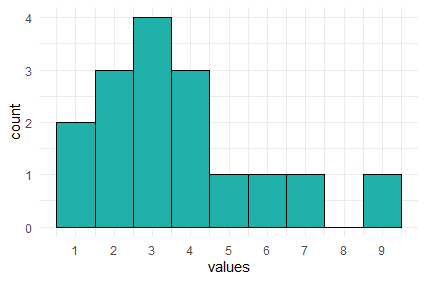
\includegraphics{./img/hist1.png}

In this histogram, the height of each bar represents the total amount of
the number on the x-axis. So, the height of the bar at \texttt{x=9} is
one. This mean we have 1 of this value in our data distribution. The
height of the bar at \texttt{x=3} is four, therefore we have four in our
distribution for the value 3.

In the example above, the width of the bars is precisely 1. We could
change the width to say two. This is illustrated below:

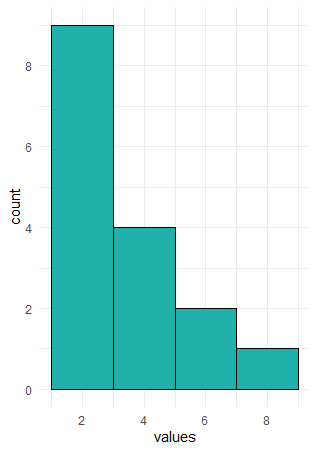
\includegraphics{./img/hist2.png}

Here, the first bar is at height 9. It spans the values of x between
1-3. The second bar is at height 4, this include values between 3.01-5,
and so on. What we did here was to adjust the \texttt{binwidth}. When we
have large distributions, adjusting the binwidth helps us to interpret
the data more easily.

\hypertarget{histograms-with-ggplot2}{%
\section{Histograms with ggplot2}\label{histograms-with-ggplot2}}

To describe how to make histograms with the \texttt{ggplot()} function,
lets look at the \texttt{films.csv} dataset.

\begin{Shaded}
\begin{Highlighting}[]
\FunctionTok{library}\NormalTok{(tidyverse)}
\NormalTok{film }\OtherTok{\textless{}{-}} \FunctionTok{read\_csv}\NormalTok{(}\StringTok{"data\_raw/films.csv"}\NormalTok{)}
\FunctionTok{head}\NormalTok{(film)}
\end{Highlighting}
\end{Shaded}

\begin{verbatim}
# A tibble: 6 x 5
  film                     year rottentomatoes  imdb metacritic
  <chr>                   <dbl>          <dbl> <dbl>      <dbl>
1 Avengers: Age of Ultron  2015             74   7.8         66
2 Cinderella               2015             85   7.1         67
3 Ant-Man                  2015             80   7.8         64
4 Do You Believe?          2015             18   5.4         22
5 Hot Tub Time Machine 2   2015             14   5.1         29
6 The Water Diviner        2015             63   7.2         50
\end{verbatim}

This dataset contains 146 rows of data. Each row has a unique film, with
the final three columns giving three different ratings measures of how
good the film was. These are their respective \texttt{rottentomatoes},
\texttt{imdb} and \texttt{metacritic} scores.

If we wished to plot the distribution of \texttt{imdb} scores, we need
to put \texttt{x=imdb} inside the \texttt{aes()} part of the ggplot
code. That is to tell it to plot these scores on the x-axis. We do not
need to put a \texttt{y=} inside this, as we are not plotting anything
from our dataset on the y-axis. Instead, ggplot2 will count up the
frequency of our scores between regular intervals of \texttt{imdb}
scores.

We then add \texttt{+\ geom\_histogram()} to tell it to make a
histogram. All together it looks like this:

\begin{Shaded}
\begin{Highlighting}[]
\FunctionTok{ggplot}\NormalTok{(film, }\FunctionTok{aes}\NormalTok{(}\AttributeTok{x=}\NormalTok{imdb)) }\SpecialCharTok{+} 
  \FunctionTok{geom\_histogram}\NormalTok{()  }
\end{Highlighting}
\end{Shaded}

\begin{verbatim}
`stat_bin()` using `bins = 30`. Pick better value with `binwidth`.
\end{verbatim}

\begin{figure}[H]

{\centering \includegraphics{./histograms_files/figure-pdf/unnamed-chunk-4-1.pdf}

}

\end{figure}

Now, this doesn't look great and we have several problems with it. The
two major problems that we get with our first histograms are. 1) The
binwidth is almost never appropriate. We need to tell ggplot exactly
what we want the binwidth on the x-axis to be. That is, what interval do
we want our scores to be counted over. Looking at the graph, our scores
range from just below 4 to about 8.6. Perhaps a better interval would be
0.2, so we count how many films had scores between 3.6-3.8, 3.8-4.0,
4.0-4.2, 4.2-4.4, \ldots\ldots.. 8.4-8.6, 8.6-8.8 etc. 2) Having black
bars makes it really hard to distinguish the bars when they are close in
heights. We need to fix the color scheme.

OK, let's make the bars dodgerblue and border them white. Inside
\texttt{geom\_histogram()} we use \texttt{color="white"} to represent
the outside \emph{lines} of the bars. We use \texttt{fill="dodgerblue}
to indicate the color inside the bars should be dodgerblue.

\begin{Shaded}
\begin{Highlighting}[]
\FunctionTok{ggplot}\NormalTok{(film, }\FunctionTok{aes}\NormalTok{(}\AttributeTok{x=}\NormalTok{imdb)) }\SpecialCharTok{+} 
  \FunctionTok{geom\_histogram}\NormalTok{(}\AttributeTok{color=}\StringTok{"white"}\NormalTok{, }\AttributeTok{fill=}\StringTok{"dodgerblue"}\NormalTok{) }
\end{Highlighting}
\end{Shaded}

\begin{verbatim}
`stat_bin()` using `bins = 30`. Pick better value with `binwidth`.
\end{verbatim}

\begin{figure}[H]

{\centering \includegraphics{./histograms_files/figure-pdf/unnamed-chunk-5-1.pdf}

}

\end{figure}

Now let's fix that binwidth. To resolve this, inside
\texttt{geom\_histogram()} we write \texttt{binwidth\ =\ 0.2}.

\begin{Shaded}
\begin{Highlighting}[]
\FunctionTok{ggplot}\NormalTok{(film, }\FunctionTok{aes}\NormalTok{(}\AttributeTok{x =}\NormalTok{ imdb)) }\SpecialCharTok{+} 
  \FunctionTok{geom\_histogram}\NormalTok{(}\AttributeTok{binwidth =} \FloatTok{0.2}\NormalTok{, }\AttributeTok{color=}\StringTok{"white"}\NormalTok{, }\AttributeTok{fill=}\StringTok{"dodgerblue"}\NormalTok{) }
\end{Highlighting}
\end{Shaded}

\begin{figure}[H]

{\centering \includegraphics{./histograms_files/figure-pdf/unnamed-chunk-6-1.pdf}

}

\end{figure}

This looks a lot better. Now we can see that the majority of films have
ratings in the 6.2-7.8 range, with relatively few above 8 and below 5.
It's not always easy to know what size interval to choose for the x-axis
in histograms. It's worth just playing around with that number and
seeing how it looks.

When we set the interval to be some value - here, we chose 0.2 - R
doesn't automatically make that between easy to interpret numbers such
as 4.0-4.2, 4.2-4.4 etc. It could just as easily have chosen
3.874-4.074, 4.074-4.274. Obviously, the latter is hard for us to
interpret when looking at the axes. You can see in the above plot, that
the vertical lines of the histogram bars don't neatly fall on top of
whole numbers. To fix, this you can adjust the boundaries by picking a
value to center your interval on. So, if we pick \texttt{boundary=4},
then that will be a boundary marker, and the interval will go 4.0-4.2,
4.2-4.4 etc.

\begin{Shaded}
\begin{Highlighting}[]
\FunctionTok{ggplot}\NormalTok{(film, }\FunctionTok{aes}\NormalTok{(}\AttributeTok{x =}\NormalTok{ imdb)) }\SpecialCharTok{+} 
  \FunctionTok{geom\_histogram}\NormalTok{(}\AttributeTok{binwidth =} \FloatTok{0.2}\NormalTok{, }\AttributeTok{color=}\StringTok{"white"}\NormalTok{, }\AttributeTok{fill=}\StringTok{"dodgerblue"}\NormalTok{,}\AttributeTok{boundary=}\DecValTok{4}\NormalTok{) }
\end{Highlighting}
\end{Shaded}

\begin{figure}[H]

{\centering \includegraphics{./histograms_files/figure-pdf/unnamed-chunk-7-1.pdf}

}

\end{figure}

Just be careful with using the boundaries that it does not crop your
histogram incorrectly. Changing histograms too much can lead to
misrepresenting the data. We would recommend that you don't use the
boundary feature unless you have a real need to do so - just be careful!

Like with all ggplot figures, you can add as much customization as you
wish. Here, we add a new theme, title and x- and y-axis labels:

\begin{Shaded}
\begin{Highlighting}[]
\FunctionTok{ggplot}\NormalTok{(film, }\FunctionTok{aes}\NormalTok{(}\AttributeTok{x =}\NormalTok{ imdb)) }\SpecialCharTok{+} 
  \FunctionTok{geom\_histogram}\NormalTok{(}\AttributeTok{binwidth =} \FloatTok{0.2}\NormalTok{, }\AttributeTok{color=}\StringTok{"white"}\NormalTok{, }\AttributeTok{fill=}\StringTok{"dodgerblue"}\NormalTok{) }\SpecialCharTok{+}
  \FunctionTok{theme\_classic}\NormalTok{() }\SpecialCharTok{+}
  \FunctionTok{ggtitle}\NormalTok{(}\StringTok{"Histogram of IMDB Ratings"}\NormalTok{) }\SpecialCharTok{+}
  \FunctionTok{xlab}\NormalTok{(}\StringTok{"Rating"}\NormalTok{) }\SpecialCharTok{+}
  \FunctionTok{ylab}\NormalTok{(}\StringTok{"Frequency"}\NormalTok{)}
\end{Highlighting}
\end{Shaded}

\begin{figure}[H]

{\centering \includegraphics{./histograms_files/figure-pdf/unnamed-chunk-8-1.pdf}

}

\end{figure}

This looks really nice !

\hypertarget{density-curves}{%
\section{Density Curves}\label{density-curves}}

Instead of plotting the \textbf{frequency} or counts of values on the
y-axis, we can instead plot \textbf{density}. Here, we essentially
convert the histogram to a solid line that estimates the overall shape
of the distribution. We call this line a density curve. You can make
this plot using \texttt{ggplot()} using \texttt{+\ geom\_density()}
instead of \texttt{+\ geom\_histogram()}.

In the code below we do this for the \texttt{imdb} ratings, and we make
the line color navy, and the fill of the density curve dodgerblue:

\begin{Shaded}
\begin{Highlighting}[]
\FunctionTok{ggplot}\NormalTok{(film, }\FunctionTok{aes}\NormalTok{(}\AttributeTok{x =}\NormalTok{ imdb)) }\SpecialCharTok{+} 
  \FunctionTok{geom\_density}\NormalTok{(}\AttributeTok{color =} \StringTok{"navy"}\NormalTok{, }\AttributeTok{fill =} \StringTok{"dodgerblue"}\NormalTok{) }
\end{Highlighting}
\end{Shaded}

\begin{figure}[H]

{\centering \includegraphics{./histograms_files/figure-pdf/unnamed-chunk-9-1.pdf}

}

\end{figure}

Usually the fill of these plots is too much, so it's nice to add some
transparency. You can do that by picking a number between 0 and 1 to
provide to the \texttt{alpha} argument. Here we choose
\texttt{alpha\ =\ .4}:

\begin{Shaded}
\begin{Highlighting}[]
\FunctionTok{ggplot}\NormalTok{(film, }\FunctionTok{aes}\NormalTok{(}\AttributeTok{x =}\NormalTok{ imdb)) }\SpecialCharTok{+}  
  \FunctionTok{geom\_density}\NormalTok{(}\AttributeTok{color =} \StringTok{"navy"}\NormalTok{, }\AttributeTok{fill =} \StringTok{"dodgerblue"}\NormalTok{, }\AttributeTok{alpha=}\NormalTok{.}\DecValTok{4}\NormalTok{)}
\end{Highlighting}
\end{Shaded}

\begin{figure}[H]

{\centering \includegraphics{./histograms_files/figure-pdf/unnamed-chunk-10-1.pdf}

}

\end{figure}

The useful thing about density plots is that they give you a quick
visual aid as to the overall shape of the distribution. You can easily
see where the bulk of the data lie (here between 6 and 8 ratings score),
and whether the data is symmetrical or not.

\hypertarget{comparing-distributions}{%
\section{Comparing Distributions}\label{comparing-distributions}}

Instead of just plotting one histogram or one density curve, we often
are interested in comparing two or more distributions. This means we are
interested in comparing two or more histograms or density curves. To do
this, we first need to ensure that our data are all measured in the same
units.

\textbf{Overlaid Histograms}

To illustrate this, let's use the \texttt{lifeexp.csv} data which
contains life expectancy data for many countries.

\begin{Shaded}
\begin{Highlighting}[]
\NormalTok{life }\OtherTok{\textless{}{-}} \FunctionTok{read\_csv}\NormalTok{(}\StringTok{"data\_raw/lifeexp.csv"}\NormalTok{)}
\FunctionTok{head}\NormalTok{(life)}
\end{Highlighting}
\end{Shaded}

\begin{verbatim}
# A tibble: 6 x 6
  country     continent year      lifeExp      pop gdpPercap
  <chr>       <chr>     <chr>       <dbl>    <dbl>     <dbl>
1 Afghanistan Asia      year_1952    28.8  8425333      779.
2 Afghanistan Asia      year_2007    43.8 31889923      975.
3 Albania     Europe    year_1952    55.2  1282697     1601.
4 Albania     Europe    year_2007    76.4  3600523     5937.
5 Algeria     Africa    year_1952    43.1  9279525     2449.
6 Algeria     Africa    year_2007    72.3 33333216     6223.
\end{verbatim}

You can see that one of the columns is called \texttt{lifeExp} which is
the life expectancy of each country in either 1952 or 2007. The year is
shown in the \texttt{year} column, and the country is shown in the
\texttt{country} column. You'll notice that these data are in long
format.

Perhaps we are interested in the distribution of life expectancies
across all countries in the year 1952 compared to the distribution of
life expectancies in the year 2007. We have a few options to do this.

The first option does not look good for this example (although it may
work in other situations). This is an \textbf{overlaid histogram}. To do
this, inside \texttt{aes()} as well as saying which column our
distribution data is in \texttt{x=lifeExp}, we also tell it to make
separate histograms based on the year column with \texttt{fill=year}.
This will ensure it uses different fill colors for the two different
years. Although not necessary, putting \texttt{position="identity"}
inside \texttt{geom\_histogram()} helps make the plot a little nicer.
Putting \texttt{color="black"} and \texttt{alpha=.7} inside
\texttt{geom\_histogram()} also helps distinguish the two histograms.

\begin{Shaded}
\begin{Highlighting}[]
\FunctionTok{ggplot}\NormalTok{(life, }\FunctionTok{aes}\NormalTok{(}\AttributeTok{x=}\NormalTok{lifeExp, }\AttributeTok{fill=}\NormalTok{year)) }\SpecialCharTok{+}  
  \FunctionTok{geom\_histogram}\NormalTok{(}\AttributeTok{binwidth=}\DecValTok{2}\NormalTok{, }\AttributeTok{position=}\StringTok{"identity"}\NormalTok{, }\AttributeTok{color=}\StringTok{"black"}\NormalTok{, }\AttributeTok{alpha=}\NormalTok{.}\DecValTok{7}\NormalTok{) }\SpecialCharTok{+}
  \FunctionTok{theme\_minimal}\NormalTok{()}
\end{Highlighting}
\end{Shaded}

\begin{figure}[H]

{\centering \includegraphics{./histograms_files/figure-pdf/unnamed-chunk-12-1.pdf}

}

\end{figure}

This plot is still pretty bad though. This method of plotting is better
when the histograms are quite distinctive from one another and there
isn't much overlap in the distributions.

Choosing two colors that contrast more strongly than the default colors
can help. Here, we are using hexcodes to pick a gray and a mustard
yellow color. We manually define our fill colors using
\texttt{+\ \ scale\_fill\_manual(values\ =\ c("\#999999",\ "\#E69F00"))}.
To change the colors, just change the hexcodes to different ones or the
names of colors you'd like. Just make sure that you have the same number
of colors as groups in your data. Here, we have two groups (1952 and
2007) so we need two colors. Also, notice that it says
\texttt{scale\_fill\_manual} and not \texttt{scale\_color\_manual}.
Because we are dealing with the inside color - this is considered to be
a \textbf{fill} in ggplot2 terms. We used \texttt{fill=year} inside
\texttt{aes()} so we need to match that with \texttt{fill} when manually
choosing colors.

\begin{Shaded}
\begin{Highlighting}[]
\FunctionTok{ggplot}\NormalTok{(life, }\FunctionTok{aes}\NormalTok{(}\AttributeTok{x=}\NormalTok{lifeExp, }\AttributeTok{fill=}\NormalTok{year)) }\SpecialCharTok{+}  
  \FunctionTok{geom\_histogram}\NormalTok{( }\AttributeTok{binwidth=}\DecValTok{2}\NormalTok{, }\AttributeTok{position=}\StringTok{"identity"}\NormalTok{, }\AttributeTok{color=}\StringTok{"black"}\NormalTok{, }\AttributeTok{alpha=}\NormalTok{.}\DecValTok{7}\NormalTok{) }\SpecialCharTok{+}
  \FunctionTok{theme\_minimal}\NormalTok{() }\SpecialCharTok{+}
  \FunctionTok{scale\_fill\_manual}\NormalTok{(}\AttributeTok{values =} \FunctionTok{c}\NormalTok{(}\StringTok{"\#999999"}\NormalTok{, }\StringTok{"\#E69F00"}\NormalTok{))}
\end{Highlighting}
\end{Shaded}

\begin{figure}[H]

{\centering \includegraphics{./histograms_files/figure-pdf/unnamed-chunk-13-1.pdf}

}

\end{figure}

\textbf{Overlaid Density Plots}

Comparing distributions can also be done with \texttt{geom\_density}.
This is usually simpler to compare than overlaid histograms.

The default plot for this would be to include \texttt{fill=year} inside
the \texttt{aes()} code, as the \texttt{year} column contains the data
that we wish to make separate plots for.

\begin{Shaded}
\begin{Highlighting}[]
\FunctionTok{ggplot}\NormalTok{(life, }\FunctionTok{aes}\NormalTok{(}\AttributeTok{x=}\NormalTok{lifeExp, }\AttributeTok{fill=}\NormalTok{year)) }\SpecialCharTok{+}  
  \FunctionTok{geom\_density}\NormalTok{(}\AttributeTok{alpha =} \FloatTok{0.4}\NormalTok{) }
\end{Highlighting}
\end{Shaded}

\begin{figure}[H]

{\centering \includegraphics{./histograms_files/figure-pdf/unnamed-chunk-14-1.pdf}

}

\end{figure}

We can add a custom fill colors with
\texttt{+\ scale\_fill\_manual(values\ =\ c("\#999999",\ "\#E69F00"))}
and a custom theme with \texttt{+\ theme\_classic()}.

\begin{Shaded}
\begin{Highlighting}[]
\FunctionTok{ggplot}\NormalTok{(life, }\FunctionTok{aes}\NormalTok{(}\AttributeTok{x=}\NormalTok{lifeExp, }\AttributeTok{fill=}\NormalTok{year)) }\SpecialCharTok{+}  
  \FunctionTok{geom\_density}\NormalTok{(}\FunctionTok{aes}\NormalTok{(}\AttributeTok{fill =}\NormalTok{ year), }\AttributeTok{alpha =} \FloatTok{0.4}\NormalTok{) }\SpecialCharTok{+}
  \FunctionTok{scale\_fill\_manual}\NormalTok{(}\AttributeTok{values =} \FunctionTok{c}\NormalTok{(}\StringTok{"\#999999"}\NormalTok{, }\StringTok{"\#E69F00"}\NormalTok{))  }\SpecialCharTok{+} 
  \FunctionTok{theme\_classic}\NormalTok{()}
\end{Highlighting}
\end{Shaded}

\begin{figure}[H]

{\centering \includegraphics{./histograms_files/figure-pdf/unnamed-chunk-15-1.pdf}

}

\end{figure}

This plot is now very easy to interpret. It's clear that in 2007 most
countries had life expectancies of over 70, with a tail towards younger
life expectancies. In 1952, the opposite pattern is found with most
countries having life expectancies around 40 with the tail going towards
older countries.

\hypertarget{stem-and-leaf-plots}{%
\section{Stem-and-Leaf Plots}\label{stem-and-leaf-plots}}

Stem-and-leaf plots are a simplistic version of histograms. Before the
advent of computers, this kind of plot would sometimes be easier to make
than a histogram. Their heyday was quite a few decades ago! In fact,
nowadays, these types of plots are almost never made by researchers or
data scientists in the real world. They are pretty much exclusive to
introductory statistics courses. This is a bit of a shame because we
think they are pretty cute.

Here is an example. Imagine we have the following numbers in a
distribution. They may represent temperatures:

\texttt{20,\ 20,\ 23,\ 28,\ 29,\ 31,\ 32,\ 39,\ 40,\ 41,\ 42,\ 44,\ 44,\ 45,\ 48,\ 49,\ 55,\ 55,\ 56,\ 58,\ 59,\ 61,\ 62,\ 65,\ 66,\ 67,\ 70,\ 71,\ 75,\ 82,\ 86}

We can represent these in a stem-and-leaf plot as below. The first
column represents the ``tens'' and the second column represents the
``ones''. So the ``6'' in the last row in the second column represents a
temperature of 86. We put the second column data in ascending order. The
heights of these bars represent a kind of histogram of sorts.

\includegraphics{./img/sl1.png}

The columns do not have to be tens and ones. For instance, if our data
had been seconds, and the distribution was
\texttt{2.0,\ 2.0,\ 2.3,\ 2.8.......\ 7.5,\ 8.2,\ 8.6} we could have
done the same stem-and-leaf plot.

There isn't a simple ggplot way of making stem-and-leaf plots, but there
is a built-in function called \texttt{stem()} that can make them.

For an example, if we return to our imdb ratings:

\begin{Shaded}
\begin{Highlighting}[]
\FunctionTok{head}\NormalTok{(film)}
\end{Highlighting}
\end{Shaded}

\begin{verbatim}
# A tibble: 6 x 5
  film                     year rottentomatoes  imdb metacritic
  <chr>                   <dbl>          <dbl> <dbl>      <dbl>
1 Avengers: Age of Ultron  2015             74   7.8         66
2 Cinderella               2015             85   7.1         67
3 Ant-Man                  2015             80   7.8         64
4 Do You Believe?          2015             18   5.4         22
5 Hot Tub Time Machine 2   2015             14   5.1         29
6 The Water Diviner        2015             63   7.2         50
\end{verbatim}

We can make a stem-and-leaf plot of the \texttt{imdb} column like this.
The \texttt{scale=0.6} parameter dictates how long the stem-and-leaf
plot should be. You can adjust it to your liking. Lower numbers make the
plot shorter:

\begin{Shaded}
\begin{Highlighting}[]
\FunctionTok{stem}\NormalTok{(film}\SpecialCharTok{$}\NormalTok{imdb, }\AttributeTok{scale=}\FloatTok{0.6}\NormalTok{)}
\end{Highlighting}
\end{Shaded}

\begin{verbatim}

  The decimal point is at the |

  4 | 0234
  4 | 6699
  5 | 01224444
  5 | 555556678999
  6 | 0011112333333333444444
  6 | 5555666666666777777789999999
  7 | 0000111111122222222223333344444444
  7 | 555555666777788888888899
  8 | 012222344
  8 | 6
\end{verbatim}

Here, the lowest rating we have is 4.0, and the highest is 8.6.

\bookmarksetup{startatroot}

\hypertarget{distributions-across-groups}{%
\chapter{Distributions Across
Groups}\label{distributions-across-groups}}

One of the most important data visualizations that we make is to compare
the distribution of data across groups. Here we have a categorical
variable on the x-axis, and a continuous variable on the y-axis. For
some reason, the most common way to represent these data in most of the
scientific literature is to plot bar graphs with error bars - so-called
dynamite plots. However, in our very strong opinion these plots are
dreadful and you should never use them.
\href{http://biostat.mc.vanderbilt.edu/wiki/pub/Main/TatsukiRcode/Poster3.pdf}{Fortunately
others agree}. Instead, please choose from strip plots, boxplots or
violin plots, or a combination, depending upon your data.

In this section we'll use the \texttt{wheels1.csv} dataset. These data
show the number of revolutions of a running wheel made by mice over a
four day period. The mice vary by their strain (type). Here we just
select the \texttt{id}, \texttt{strain} and \texttt{day4} columns for
this example:

\begin{Shaded}
\begin{Highlighting}[]
\FunctionTok{library}\NormalTok{(tidyverse)}
\NormalTok{wheels }\OtherTok{\textless{}{-}} \FunctionTok{read\_csv}\NormalTok{(}\StringTok{"data\_raw/wheels1.csv"}\NormalTok{)}
\NormalTok{wheels1 }\OtherTok{\textless{}{-}}\NormalTok{ wheels }\SpecialCharTok{\%\textgreater{}\%} \FunctionTok{select}\NormalTok{(id, strain, day4) }
\FunctionTok{head}\NormalTok{(wheels1)}
\end{Highlighting}
\end{Shaded}

\begin{verbatim}
# A tibble: 6 x 3
  id    strain   day4
  <chr> <chr>   <dbl>
1 692ao B6     12516.
2 656aa B6      7404.
3 675ag B6      3761 
4 675ai B6     11684 
5 656af B6      8468.
6 656al B6      9291 
\end{verbatim}

The \texttt{day4} column represents how many wheel revolutions the mice
made on their fourth day running in the wheel. Some mice really like
running in the wheel, others aren't as bothered!

Let's have a look at how many datapoints we have in each strain:

\begin{Shaded}
\begin{Highlighting}[]
\FunctionTok{table}\NormalTok{(wheels}\SpecialCharTok{$}\NormalTok{strain)}
\end{Highlighting}
\end{Shaded}

\begin{verbatim}

      B6 F1-129B6 F1-B6129     S129    Swiss 
      14       22       15       16       13 
\end{verbatim}

We have 80 mice in five different strains.

\hypertarget{strip-plots}{%
\section{Strip Plots}\label{strip-plots}}

Strip plots essentially just plot the raw data. It's like plotting a
scatterplot, except we plot a categorical variable on the x-axis.

So in our example, inside \texttt{aes()} we'll put strain on the x-axis
with \texttt{x=strain}, and on the y-axis we put our outcome variable
with \texttt{y=day4}. We'll add datapoints with
\texttt{+\ geom\_point()}:

\begin{Shaded}
\begin{Highlighting}[]
\FunctionTok{ggplot}\NormalTok{(wheels1, }\FunctionTok{aes}\NormalTok{(}\AttributeTok{x =}\NormalTok{ strain, }\AttributeTok{y =}\NormalTok{ day4)) }\SpecialCharTok{+} 
  \FunctionTok{geom\_point}\NormalTok{()  }\SpecialCharTok{+}
  \FunctionTok{theme\_classic}\NormalTok{()}
\end{Highlighting}
\end{Shaded}

\begin{figure}[H]

{\centering \includegraphics{./distributionsgroups_files/figure-pdf/unnamed-chunk-3-1.pdf}

}

\end{figure}

The major issue with this plot is that all the points are in a very
straight line, and it can be difficult to distinguish between different
points. To change this, instead of using \texttt{geom\_point()} we use
\texttt{geom\_jitter()} which bounces the points around a bit:

\begin{Shaded}
\begin{Highlighting}[]
\FunctionTok{ggplot}\NormalTok{(wheels1, }\FunctionTok{aes}\NormalTok{(}\AttributeTok{x =}\NormalTok{ strain, }\AttributeTok{y =}\NormalTok{ day4)) }\SpecialCharTok{+} 
  \FunctionTok{geom\_jitter}\NormalTok{()  }\SpecialCharTok{+}
  \FunctionTok{theme\_classic}\NormalTok{()}
\end{Highlighting}
\end{Shaded}

\begin{figure}[H]

{\centering \includegraphics{./distributionsgroups_files/figure-pdf/unnamed-chunk-4-1.pdf}

}

\end{figure}

Whoops! The points exploded. Now it's not possible to know which points
belong to which group. To constrain this, we can set \texttt{width=}
inside of \texttt{geom\_jitter()} which tells the points how far they
are allowed to bounce around:

\begin{Shaded}
\begin{Highlighting}[]
\FunctionTok{ggplot}\NormalTok{(wheels1, }\FunctionTok{aes}\NormalTok{(}\AttributeTok{x =}\NormalTok{ strain, }\AttributeTok{y =}\NormalTok{ day4)) }\SpecialCharTok{+} 
  \FunctionTok{geom\_jitter}\NormalTok{(}\AttributeTok{width =}\NormalTok{ .}\DecValTok{15}\NormalTok{)  }\SpecialCharTok{+}
  \FunctionTok{theme\_classic}\NormalTok{()}
\end{Highlighting}
\end{Shaded}

\begin{figure}[H]

{\centering \includegraphics{./distributionsgroups_files/figure-pdf/unnamed-chunk-5-1.pdf}

}

\end{figure}

This looks a lot better!.

\hypertarget{boxplots}{%
\section{Boxplots}\label{boxplots}}

Boxplots are a very useful way of summarizing the distribution of data.
The image below summarizes what each line in the boxplot represents.

\includegraphics{./img/box2.png}

The middle horizontal line is at 6. This represents the \textbf{median}
of the distribution which is the middle value. 50\% of the distribution
lies above this value and 50\% below it. The higher horizontal line at
the top of the box represents the \textbf{upper quartile}. This is
approximately the median of the upper 50\% of the data, so is
approximately the 75\% percentile. The lower horizontal line at the
bottom of the box represents the \textbf{lower quartile}. This is
approximately the median of the lower 50\% of the data, so is
approximately the 25\% percentile of the data. Therefore, the middle
50\% of the data (from the 25\% percentile to the 75\% percentile) lies
inside the box. The long vertical lines represent the \textbf{range} of
the data. The top of that line is the maximum value in the data, and the
bottom of that line is the minimum value in the distribution.

The above is a basic boxplot. However, \texttt{ggplot2} does things a
little bit differently. It turns out there is more than one way to
calculate the lower and upper quartiles (see section
@ref(interquartile-range)). Also, R doesn't necessarily extend the
vertical lines (\textbf{whiskers}) all the way to the minimum and
maximum values. If there are datapoints that are too far away from the
upper or lower quartile, then it truncates the whisker and shows
datapoints outside of this range as dots. Here is an illustration of a
ggplot boxplot:

\includegraphics{./img/box3.png}

OK, let's have a look at some boxplots using \texttt{ggplot()}. We
provide the same \texttt{x=strain} and \texttt{y=day4} values as we do
with strip plots. Instead of \texttt{geom\_jitter()} we use
\texttt{geom\_boxplot()}:

\begin{Shaded}
\begin{Highlighting}[]
\FunctionTok{ggplot}\NormalTok{(wheels1, }\FunctionTok{aes}\NormalTok{(}\AttributeTok{x =}\NormalTok{ strain, }\AttributeTok{y =}\NormalTok{ day4)) }\SpecialCharTok{+} 
  \FunctionTok{geom\_boxplot}\NormalTok{()  }\SpecialCharTok{+}
  \FunctionTok{theme\_classic}\NormalTok{()}
\end{Highlighting}
\end{Shaded}

\begin{figure}[H]

{\centering \includegraphics{./distributionsgroups_files/figure-pdf/unnamed-chunk-6-1.pdf}

}

\end{figure}

You can see in this example, that the strain ``F1-129B6'' and the strain
``S129'' both have two datapoints that are shown as outliers beyond the
whiskers.

To change the colors of the boxplots, you can change \texttt{color=} and
\texttt{fill=} inside \texttt{geom\_boxplot()}. Remember that
\texttt{color} refers to the color of the lines, and \texttt{fill}
refers to the filled in color of the shape:

\begin{Shaded}
\begin{Highlighting}[]
\FunctionTok{ggplot}\NormalTok{(wheels1, }\FunctionTok{aes}\NormalTok{(}\AttributeTok{x =}\NormalTok{ strain, }\AttributeTok{y =}\NormalTok{ day4)) }\SpecialCharTok{+} 
  \FunctionTok{geom\_boxplot}\NormalTok{(}\AttributeTok{color=}\StringTok{"navy"}\NormalTok{, }\AttributeTok{fill=}\StringTok{"lightsteelblue1"}\NormalTok{) }\SpecialCharTok{+}
  \FunctionTok{theme\_classic}\NormalTok{()}
\end{Highlighting}
\end{Shaded}

\begin{figure}[H]

{\centering \includegraphics{./distributionsgroups_files/figure-pdf/unnamed-chunk-7-1.pdf}

}

\end{figure}

You can change the size, color and shape of the outliers. For instance,
to remove them completely, we do \texttt{outlier.shape=NA} inside
\texttt{geom\_boxplot()}

\begin{Shaded}
\begin{Highlighting}[]
\FunctionTok{ggplot}\NormalTok{(wheels1, }\FunctionTok{aes}\NormalTok{(}\AttributeTok{x =}\NormalTok{ strain, }\AttributeTok{y =}\NormalTok{ day4)) }\SpecialCharTok{+} 
  \FunctionTok{geom\_boxplot}\NormalTok{(}\AttributeTok{color=}\StringTok{"navy"}\NormalTok{, }\AttributeTok{fill=}\StringTok{"lightsteelblue1"}\NormalTok{, }\AttributeTok{outlier.shape =} \ConstantTok{NA}\NormalTok{) }\SpecialCharTok{+}
  \FunctionTok{theme\_classic}\NormalTok{()}
\end{Highlighting}
\end{Shaded}

\begin{figure}[H]

{\centering \includegraphics{./distributionsgroups_files/figure-pdf/unnamed-chunk-8-1.pdf}

}

\end{figure}

To change the size and color, you can use \texttt{outlier.size} and
\texttt{outlier.color} respectively inside \texttt{geom\_boxplot()}

\begin{Shaded}
\begin{Highlighting}[]
\FunctionTok{ggplot}\NormalTok{(wheels1, }\FunctionTok{aes}\NormalTok{(}\AttributeTok{x =}\NormalTok{ strain, }\AttributeTok{y =}\NormalTok{ day4)) }\SpecialCharTok{+} 
  \FunctionTok{geom\_boxplot}\NormalTok{(}\AttributeTok{color=}\StringTok{"navy"}\NormalTok{, }\AttributeTok{fill=}\StringTok{"lightsteelblue1"}\NormalTok{, }\AttributeTok{outlier.size =}\NormalTok{ .}\DecValTok{5}\NormalTok{, }\AttributeTok{outlier.color =} \StringTok{"gray66"}\NormalTok{) }\SpecialCharTok{+}
  \FunctionTok{theme\_classic}\NormalTok{()}
\end{Highlighting}
\end{Shaded}

\begin{figure}[H]

{\centering \includegraphics{./distributionsgroups_files/figure-pdf/unnamed-chunk-9-1.pdf}

}

\end{figure}

\hypertarget{overlaying-points}{%
\subsection{Overlaying points}\label{overlaying-points}}

It can often be helpful to overlay your raw datapoints over the top of
boxplots, providing that you don't have too much data. To do this, just
add your points with either \texttt{geom\_point()} or preferably
\texttt{geom\_jitter()}. But one warning - make sure you remove any
outliers with \texttt{outlier.shape=NA} otherwise those datapoints will
show up twice:

\begin{Shaded}
\begin{Highlighting}[]
\FunctionTok{ggplot}\NormalTok{(wheels1, }\FunctionTok{aes}\NormalTok{(}\AttributeTok{x =}\NormalTok{ strain, }\AttributeTok{y =}\NormalTok{ day4)) }\SpecialCharTok{+} 
  \FunctionTok{geom\_boxplot}\NormalTok{(}\AttributeTok{color=}\StringTok{"navy"}\NormalTok{, }\AttributeTok{fill=}\StringTok{"lightsteelblue1"}\NormalTok{, }\AttributeTok{outlier.shape =} \ConstantTok{NA}\NormalTok{) }\SpecialCharTok{+}
  \FunctionTok{geom\_jitter}\NormalTok{(}\AttributeTok{width=}\FloatTok{0.15}\NormalTok{, }\AttributeTok{color=}\StringTok{"navy"}\NormalTok{) }\SpecialCharTok{+}
  \FunctionTok{theme\_classic}\NormalTok{()}
\end{Highlighting}
\end{Shaded}

\begin{figure}[H]

{\centering \includegraphics{./distributionsgroups_files/figure-pdf/unnamed-chunk-10-1.pdf}

}

\end{figure}

Sometimes this can look a bit too busy. One way to contrast things is to
set either the points or the boxplots themselves to have some
transparency with \texttt{alpha=}.

Here we make the points a bit transparent:

\begin{Shaded}
\begin{Highlighting}[]
\FunctionTok{ggplot}\NormalTok{(wheels1, }\FunctionTok{aes}\NormalTok{(}\AttributeTok{x =}\NormalTok{ strain, }\AttributeTok{y =}\NormalTok{ day4)) }\SpecialCharTok{+} 
  \FunctionTok{geom\_boxplot}\NormalTok{(}\AttributeTok{color=}\StringTok{"navy"}\NormalTok{, }\AttributeTok{fill=}\StringTok{"lightsteelblue1"}\NormalTok{, }\AttributeTok{outlier.shape =} \ConstantTok{NA}\NormalTok{) }\SpecialCharTok{+}
  \FunctionTok{geom\_jitter}\NormalTok{(}\AttributeTok{width=}\FloatTok{0.15}\NormalTok{, }\AttributeTok{color=}\StringTok{"navy"}\NormalTok{, }\AttributeTok{alpha =}\NormalTok{ .}\DecValTok{3}\NormalTok{) }\SpecialCharTok{+}
  \FunctionTok{theme\_classic}\NormalTok{()}
\end{Highlighting}
\end{Shaded}

\begin{figure}[H]

{\centering \includegraphics{./distributionsgroups_files/figure-pdf/unnamed-chunk-11-1.pdf}

}

\end{figure}

Here we leave the points solid, but make the boxplot fill transparent:

\begin{Shaded}
\begin{Highlighting}[]
\FunctionTok{ggplot}\NormalTok{(wheels1, }\FunctionTok{aes}\NormalTok{(}\AttributeTok{x =}\NormalTok{ strain, }\AttributeTok{y =}\NormalTok{ day4)) }\SpecialCharTok{+} 
  \FunctionTok{geom\_boxplot}\NormalTok{(}\AttributeTok{color=}\StringTok{"navy"}\NormalTok{, }\AttributeTok{fill=}\StringTok{"lightsteelblue1"}\NormalTok{, }\AttributeTok{outlier.shape =} \ConstantTok{NA}\NormalTok{, }\AttributeTok{alpha =}\NormalTok{ .}\DecValTok{3}\NormalTok{) }\SpecialCharTok{+}
  \FunctionTok{geom\_jitter}\NormalTok{(}\AttributeTok{width=}\FloatTok{0.15}\NormalTok{, }\AttributeTok{color=}\StringTok{"navy"}\NormalTok{) }\SpecialCharTok{+}
  \FunctionTok{theme\_classic}\NormalTok{()}
\end{Highlighting}
\end{Shaded}

\begin{figure}[H]

{\centering \includegraphics{./distributionsgroups_files/figure-pdf/unnamed-chunk-12-1.pdf}

}

\end{figure}

And finally, making both a bit transparent, adding some custom titles
and labels. You can just choose what you think looks best!

\begin{Shaded}
\begin{Highlighting}[]
\FunctionTok{ggplot}\NormalTok{(wheels1, }\FunctionTok{aes}\NormalTok{(}\AttributeTok{x =}\NormalTok{ strain, }\AttributeTok{y =}\NormalTok{ day4)) }\SpecialCharTok{+} 
  \FunctionTok{geom\_boxplot}\NormalTok{(}\AttributeTok{color=}\StringTok{"navy"}\NormalTok{, }\AttributeTok{fill=}\StringTok{"lightsteelblue1"}\NormalTok{, }\AttributeTok{outlier.shape =} \ConstantTok{NA}\NormalTok{, }\AttributeTok{alpha =}\NormalTok{ .}\DecValTok{3}\NormalTok{) }\SpecialCharTok{+}
  \FunctionTok{geom\_jitter}\NormalTok{(}\AttributeTok{width=}\FloatTok{0.15}\NormalTok{, }\AttributeTok{color=}\StringTok{"navy"}\NormalTok{, }\AttributeTok{alpha=}\NormalTok{.}\DecValTok{3}\NormalTok{) }\SpecialCharTok{+}
  \FunctionTok{theme\_classic}\NormalTok{()  }\SpecialCharTok{+}
  \FunctionTok{xlab}\NormalTok{(}\StringTok{"Mouse Strain"}\NormalTok{) }\SpecialCharTok{+}
  \FunctionTok{ylab}\NormalTok{(}\StringTok{"Total Revolutions"}\NormalTok{) }\SpecialCharTok{+}
  \FunctionTok{ggtitle}\NormalTok{(}\StringTok{"Mouse Wheel Running"}\NormalTok{)}
\end{Highlighting}
\end{Shaded}

\begin{figure}[H]

{\centering \includegraphics{./distributionsgroups_files/figure-pdf/unnamed-chunk-13-1.pdf}

}

\end{figure}

\hypertarget{reordering-categorical-x-axes}{%
\subsection{Reordering categorical
x-axes}\label{reordering-categorical-x-axes}}

The boxplot that we made looks ok, but one thing is visually annoying.
The boxes are plotted in alphabetical order on the x-axis (B6,
F1-129B6\ldots.. Swiss). There is no reason why they should be in this
order. A more visually appealing way would be to order the boxplots from
the group with the highest median to the lowest median.

To do this, instead of putting \texttt{x=strain} inside of
\texttt{aes()} we put \texttt{x\ =\ reorder(strain,\ -day4,\ median)}
inside instead. This is a bit of a mouthful. To break it down, it's
saying plot strain on the x-axis, but reorder the groups based on the
median of the strain column (that's the `-day4' in the code).

\begin{Shaded}
\begin{Highlighting}[]
\FunctionTok{ggplot}\NormalTok{(wheels1, }\FunctionTok{aes}\NormalTok{(}\AttributeTok{x =} \FunctionTok{reorder}\NormalTok{(strain, }\SpecialCharTok{{-}}\NormalTok{day4, median), }\AttributeTok{y =}\NormalTok{ day4)) }\SpecialCharTok{+} 
  \FunctionTok{geom\_boxplot}\NormalTok{(}\AttributeTok{color=}\StringTok{"navy"}\NormalTok{, }\AttributeTok{fill=}\StringTok{"lightsteelblue1"}\NormalTok{, }\AttributeTok{alpha =}\NormalTok{ .}\DecValTok{3}\NormalTok{) }\SpecialCharTok{+}
  \FunctionTok{theme\_classic}\NormalTok{()}
\end{Highlighting}
\end{Shaded}

\begin{figure}[H]

{\centering \includegraphics{./distributionsgroups_files/figure-pdf/unnamed-chunk-14-1.pdf}

}

\end{figure}

The output looks pretty good - it is now really easy to notice that one
of the groups has a much lower distribution than the others. The major
issue is that the label of the x-axis is terrible. So let's fix that:

\begin{Shaded}
\begin{Highlighting}[]
\FunctionTok{ggplot}\NormalTok{(wheels1, }\FunctionTok{aes}\NormalTok{(}\AttributeTok{x =} \FunctionTok{reorder}\NormalTok{(strain, }\SpecialCharTok{{-}}\NormalTok{day4, median), }\AttributeTok{y =}\NormalTok{ day4)) }\SpecialCharTok{+} 
  \FunctionTok{geom\_boxplot}\NormalTok{(}\AttributeTok{color=}\StringTok{"navy"}\NormalTok{, }\AttributeTok{fill=}\StringTok{"lightsteelblue1"}\NormalTok{, }\AttributeTok{alpha =}\NormalTok{ .}\DecValTok{3}\NormalTok{) }\SpecialCharTok{+}
  \FunctionTok{theme\_classic}\NormalTok{() }\SpecialCharTok{+}
  \FunctionTok{xlab}\NormalTok{(}\StringTok{"Mouse Strain"}\NormalTok{) }\SpecialCharTok{+}
  \FunctionTok{ylab}\NormalTok{(}\StringTok{"Total Revolutions"}\NormalTok{) }\SpecialCharTok{+}
  \FunctionTok{ggtitle}\NormalTok{(}\StringTok{"Mouse Wheel Running"}\NormalTok{)}
\end{Highlighting}
\end{Shaded}

\begin{figure}[H]

{\centering \includegraphics{./distributionsgroups_files/figure-pdf/unnamed-chunk-15-1.pdf}

}

\end{figure}

Much nicer!

\hypertarget{flipping-axes}{%
\subsection{Flipping Axes}\label{flipping-axes}}

Often boxplots look perfectly fine with the categorical grouping
variable on the x-axis and the continuous variable on the y-axis. If you
start to have many groups, then sometimes the boxplots looks too
cluttered when placed on the x-axis. In this situation, it might look
better to flip the axes, and have the boxplots stacked vertically. To do
this, you write your plot code exactly as you would normally, but you
just add \texttt{+\ coord\_flip()} to the end of the code.

Let's add this to the reordered boxplots we just made in the previous
section:

\begin{Shaded}
\begin{Highlighting}[]
\FunctionTok{ggplot}\NormalTok{(wheels1, }\FunctionTok{aes}\NormalTok{(}\AttributeTok{x =} \FunctionTok{reorder}\NormalTok{(strain, }\SpecialCharTok{{-}}\NormalTok{day4, median), }\AttributeTok{y =}\NormalTok{ day4)) }\SpecialCharTok{+} 
  \FunctionTok{geom\_boxplot}\NormalTok{(}\AttributeTok{color=}\StringTok{"navy"}\NormalTok{, }\AttributeTok{fill=}\StringTok{"lightsteelblue1"}\NormalTok{, }\AttributeTok{alpha =}\NormalTok{ .}\DecValTok{3}\NormalTok{) }\SpecialCharTok{+}
  \FunctionTok{theme\_classic}\NormalTok{() }\SpecialCharTok{+}
  \FunctionTok{xlab}\NormalTok{(}\StringTok{"Mouse Strain"}\NormalTok{) }\SpecialCharTok{+}
  \FunctionTok{ylab}\NormalTok{(}\StringTok{"Total Revolutions"}\NormalTok{) }\SpecialCharTok{+}
  \FunctionTok{ggtitle}\NormalTok{(}\StringTok{"Mouse Wheel Running"}\NormalTok{) }\SpecialCharTok{+}
  \FunctionTok{coord\_flip}\NormalTok{()}
\end{Highlighting}
\end{Shaded}

\begin{figure}[H]

{\centering \includegraphics{./distributionsgroups_files/figure-pdf/unnamed-chunk-16-1.pdf}

}

\end{figure}

This is OK, but it would be nicer if the highest values were at the top.
There may well be a more straightforward way of doing this, but a quick
solution is to wrap \texttt{reorder(strain,\ strain,\ median)} with
\texttt{fct\_rev}, so you now have
\texttt{x\ =\ fct\_rev(reorder(strain,\ strain,\ median))}. It's a whole
lot of code, but it does make the graph really pretty, so it's worth it:

\begin{Shaded}
\begin{Highlighting}[]
\FunctionTok{ggplot}\NormalTok{(wheels1, }\FunctionTok{aes}\NormalTok{(}\AttributeTok{x =} \FunctionTok{fct\_rev}\NormalTok{(}\FunctionTok{reorder}\NormalTok{(strain, }\SpecialCharTok{{-}}\NormalTok{day4, median)), }\AttributeTok{y =}\NormalTok{ day4)) }\SpecialCharTok{+} 
  \FunctionTok{geom\_boxplot}\NormalTok{(}\AttributeTok{color=}\StringTok{"navy"}\NormalTok{, }\AttributeTok{fill=}\StringTok{"lightsteelblue1"}\NormalTok{, }\AttributeTok{alpha =}\NormalTok{ .}\DecValTok{3}\NormalTok{) }\SpecialCharTok{+}
  \FunctionTok{theme\_classic}\NormalTok{() }\SpecialCharTok{+}
  \FunctionTok{xlab}\NormalTok{(}\StringTok{"Mouse Strain"}\NormalTok{) }\SpecialCharTok{+}
  \FunctionTok{ylab}\NormalTok{(}\StringTok{"Total Revolutions"}\NormalTok{) }\SpecialCharTok{+}
  \FunctionTok{ggtitle}\NormalTok{(}\StringTok{"Mouse Wheel Running"}\NormalTok{) }\SpecialCharTok{+}
  \FunctionTok{coord\_flip}\NormalTok{() }
\end{Highlighting}
\end{Shaded}

\begin{figure}[H]

{\centering \includegraphics{./distributionsgroups_files/figure-pdf/unnamed-chunk-17-1.pdf}

}

\end{figure}

\hypertarget{violin-plots}{%
\section{Violin Plots}\label{violin-plots}}

A disadvantage of boxplots, especially when you have large
distributions, is that the box does not tell you much about the overall
shape of the distribution. An alternative are \textbf{violin plots},
where the width of the shape reflects the shape of the distribution. To
make these plots, instead of using \texttt{geom\_boxplot()} we use
\texttt{geom\_violin()}.

\begin{Shaded}
\begin{Highlighting}[]
\FunctionTok{ggplot}\NormalTok{(wheels1, }\FunctionTok{aes}\NormalTok{(}\AttributeTok{x =}\NormalTok{ strain, }\AttributeTok{y =}\NormalTok{ day4)) }\SpecialCharTok{+}  
  \FunctionTok{geom\_violin}\NormalTok{() }\SpecialCharTok{+} 
  \FunctionTok{theme\_classic}\NormalTok{()}
\end{Highlighting}
\end{Shaded}

\begin{figure}[H]

{\centering \includegraphics{./distributionsgroups_files/figure-pdf/unnamed-chunk-18-1.pdf}

}

\end{figure}

You can do all the customizing, reordering, coloring, transparency-ing,
etc that you do with boxplots:

\begin{Shaded}
\begin{Highlighting}[]
\FunctionTok{ggplot}\NormalTok{(wheels1, }\FunctionTok{aes}\NormalTok{(}\AttributeTok{x =} \FunctionTok{fct\_rev}\NormalTok{(}\FunctionTok{reorder}\NormalTok{(strain, strain, median)), }\AttributeTok{y =}\NormalTok{ day4)) }\SpecialCharTok{+} 
  \FunctionTok{geom\_violin}\NormalTok{(}\AttributeTok{color=}\StringTok{"navy"}\NormalTok{, }\AttributeTok{fill=}\StringTok{"lightsteelblue1"}\NormalTok{, }\AttributeTok{alpha =}\NormalTok{ .}\DecValTok{3}\NormalTok{) }\SpecialCharTok{+}
  \FunctionTok{theme\_classic}\NormalTok{() }\SpecialCharTok{+}
  \FunctionTok{xlab}\NormalTok{(}\StringTok{"Mouse Strain"}\NormalTok{) }\SpecialCharTok{+}
  \FunctionTok{ylab}\NormalTok{(}\StringTok{"Total Revolutions"}\NormalTok{) }\SpecialCharTok{+}
  \FunctionTok{ggtitle}\NormalTok{(}\StringTok{"Mouse Wheel Running"}\NormalTok{) }\SpecialCharTok{+}
  \FunctionTok{coord\_flip}\NormalTok{() }
\end{Highlighting}
\end{Shaded}

\begin{figure}[H]

{\centering \includegraphics{./distributionsgroups_files/figure-pdf/unnamed-chunk-19-1.pdf}

}

\end{figure}

\hypertarget{stacked-boxplots}{%
\section{Stacked Boxplots}\label{stacked-boxplots}}

Sometimes, we want to compare distributions for the same group side by
side. For instance, we may not just want to plot the day4 wheel running
data, but also plot the day1 data.

Below, we have data in \textbf{wide format}. We have ids, strain, day1
running and day4 running.

\begin{Shaded}
\begin{Highlighting}[]
\NormalTok{wheels2 }\OtherTok{\textless{}{-}}\NormalTok{ wheels }\SpecialCharTok{\%\textgreater{}\%} \FunctionTok{select}\NormalTok{(id, strain, day1, day4)}
\FunctionTok{head}\NormalTok{(wheels2)}
\end{Highlighting}
\end{Shaded}

\begin{verbatim}
# A tibble: 6 x 4
  id    strain   day1   day4
  <chr> <chr>   <dbl>  <dbl>
1 692ao B6     12853  12516.
2 656aa B6      2644   7404.
3 675ag B6      4004.  3761 
4 675ai B6     11754. 11684 
5 656af B6      6906.  8468.
6 656al B6      6517   9291 
\end{verbatim}

We need to turn this to \textbf{long data} to be able to make the
stacked boxplot graph.

\begin{Shaded}
\begin{Highlighting}[]
\NormalTok{wheels2.long }\OtherTok{\textless{}{-}}\NormalTok{ wheels2 }\SpecialCharTok{\%\textgreater{}\%} \FunctionTok{pivot\_longer}\NormalTok{(}\AttributeTok{cols =} \DecValTok{3}\SpecialCharTok{:}\DecValTok{4}\NormalTok{, }\AttributeTok{names\_to =} \StringTok{"day"}\NormalTok{)}
\NormalTok{wheels2.long}
\end{Highlighting}
\end{Shaded}

\begin{verbatim}
# A tibble: 160 x 4
   id    strain day    value
   <chr> <chr>  <chr>  <dbl>
 1 692ao B6     day1  12853 
 2 692ao B6     day4  12516.
 3 656aa B6     day1   2644 
 4 656aa B6     day4   7404.
 5 675ag B6     day1   4004.
 6 675ag B6     day4   3761 
 7 675ai B6     day1  11754.
 8 675ai B6     day4  11684 
 9 656af B6     day1   6906.
10 656af B6     day4   8468.
# ... with 150 more rows
\end{verbatim}

Now the wheel running data is in its own column - \texttt{value}. So we
use \texttt{y=value}. The grouping variable is in the \texttt{day}
column, so we use \texttt{fill=day} to make separate boxplots based on
the day. This will also make them different fill colors:

\begin{Shaded}
\begin{Highlighting}[]
\FunctionTok{ggplot}\NormalTok{(wheels2.long, }\FunctionTok{aes}\NormalTok{(}\AttributeTok{x =}\NormalTok{ strain, }\AttributeTok{y =}\NormalTok{ value, }\AttributeTok{fill=}\NormalTok{day)) }\SpecialCharTok{+} 
  \FunctionTok{geom\_boxplot}\NormalTok{() }\SpecialCharTok{+}
  \FunctionTok{theme\_classic}\NormalTok{()}
\end{Highlighting}
\end{Shaded}

\begin{figure}[H]

{\centering \includegraphics{./distributionsgroups_files/figure-pdf/unnamed-chunk-22-1.pdf}

}

\end{figure}

This looks ok, but the colors are yucky. Lets add custom titles, labels,
and we'll customize the fill colors using \texttt{scale\_fill\_manual}.
We have two groups (day1 and day4) so we need to provide two colors:

\begin{Shaded}
\begin{Highlighting}[]
\FunctionTok{ggplot}\NormalTok{(wheels2.long, }\FunctionTok{aes}\NormalTok{(}\AttributeTok{x =}\NormalTok{ strain, }\AttributeTok{y =}\NormalTok{ value, }\AttributeTok{fill=}\NormalTok{day)) }\SpecialCharTok{+} 
  \FunctionTok{geom\_boxplot}\NormalTok{() }\SpecialCharTok{+}
  \FunctionTok{theme\_classic}\NormalTok{() }\SpecialCharTok{+}
  \FunctionTok{scale\_fill\_manual}\NormalTok{(}\AttributeTok{values =} \FunctionTok{c}\NormalTok{(}\StringTok{"\#9381e3"}\NormalTok{, }\StringTok{"\#faff75"}\NormalTok{)) }\SpecialCharTok{+}
  \FunctionTok{xlab}\NormalTok{(}\StringTok{"Mouse Strain"}\NormalTok{) }\SpecialCharTok{+}
  \FunctionTok{ylab}\NormalTok{(}\StringTok{"Total Revolutions"}\NormalTok{) }\SpecialCharTok{+}
  \FunctionTok{ggtitle}\NormalTok{(}\StringTok{"Mouse Wheel Running"}\NormalTok{) }
\end{Highlighting}
\end{Shaded}

\begin{figure}[H]

{\centering \includegraphics{./distributionsgroups_files/figure-pdf/unnamed-chunk-23-1.pdf}

}

\end{figure}

It turns out all the strains increase their overall running in wheels
from day 1 to day 4, except the S129 strain who get bored with wheel
running - probably similar to how you're bored of seeing graphs about
wheel running.

\hypertarget{ridgeline-plots}{%
\section{Ridgeline Plots}\label{ridgeline-plots}}

Another useful way of displaying distributions of data across groups is
using ridgeline plots. These are essentially density histogram plots for
each categorical group plotted side by side. To do this we need to use a
package called \texttt{ggridges}. This can be installed by going to the
\texttt{Packages} tab, selecting \texttt{Install} and typing in
\texttt{ggridges} in the box.

Let's go back to the \texttt{olives} data. Say we are interested in
displaying the distribution of \texttt{oleic} acid content by
\texttt{macro.area}. We plot the categorical group of interest (here
\texttt{macro.area}) on the y-axis, and the continuous variable whose
distribution we are interested in (\texttt{oleic}) on the x-axis. We
then use \texttt{stat\_density\_ridges()} to plot the ridgeline plots.

\begin{Shaded}
\begin{Highlighting}[]
\FunctionTok{library}\NormalTok{(ggridges)}
\NormalTok{olives }\OtherTok{\textless{}{-}} \FunctionTok{read\_csv}\NormalTok{(}\StringTok{"data\_raw/olives.csv"}\NormalTok{)}
\FunctionTok{ggplot}\NormalTok{(olives, }\FunctionTok{aes}\NormalTok{(}\AttributeTok{x =}\NormalTok{ oleic, }\AttributeTok{y =}\NormalTok{ macro.area)) }\SpecialCharTok{+}
  \FunctionTok{stat\_density\_ridges}\NormalTok{() }\SpecialCharTok{+}
  \FunctionTok{theme\_classic}\NormalTok{()}
\end{Highlighting}
\end{Shaded}

\begin{figure}[H]

{\centering \includegraphics{./distributionsgroups_files/figure-pdf/unnamed-chunk-24-1.pdf}

}

\end{figure}

You can add color by adding in a \texttt{fill=} to the \texttt{aes()}.

\begin{Shaded}
\begin{Highlighting}[]
\FunctionTok{ggplot}\NormalTok{(olives, }\FunctionTok{aes}\NormalTok{(}\AttributeTok{x =}\NormalTok{ oleic, }\AttributeTok{y =}\NormalTok{ macro.area, }\AttributeTok{fill =}\NormalTok{ macro.area)) }\SpecialCharTok{+}
  \FunctionTok{stat\_density\_ridges}\NormalTok{() }\SpecialCharTok{+}
  \FunctionTok{theme\_classic}\NormalTok{() }
\end{Highlighting}
\end{Shaded}

\begin{figure}[H]

{\centering \includegraphics{./distributionsgroups_files/figure-pdf/unnamed-chunk-25-1.pdf}

}

\end{figure}

\ldots{} and perhaps we can manually override the default color scheme -
here I'm using hex codes to pick a very purply color scheme:

\begin{Shaded}
\begin{Highlighting}[]
\FunctionTok{ggplot}\NormalTok{(olives, }\FunctionTok{aes}\NormalTok{(}\AttributeTok{x =}\NormalTok{ oleic, }\AttributeTok{y =}\NormalTok{ macro.area, }\AttributeTok{fill =}\NormalTok{ macro.area)) }\SpecialCharTok{+}
  \FunctionTok{stat\_density\_ridges}\NormalTok{() }\SpecialCharTok{+}
  \FunctionTok{theme\_classic}\NormalTok{() }\SpecialCharTok{+}
  \FunctionTok{scale\_fill\_manual}\NormalTok{(}\AttributeTok{values=}\FunctionTok{c}\NormalTok{(}\StringTok{"\#D1B8D0"}\NormalTok{, }\StringTok{"\#F78EF2"}\NormalTok{, }\StringTok{"\#AC33FF"}\NormalTok{))}
\end{Highlighting}
\end{Shaded}

\begin{figure}[H]

{\centering \includegraphics{./distributionsgroups_files/figure-pdf/unnamed-chunk-26-1.pdf}

}

\end{figure}

A nice thing about these ridgeline plots is that we can easily add on
lines that represent the lower quartile, median and upper quartile by
adding in the argument \texttt{quantile\_lines\ =\ TRUE} like this:

\begin{Shaded}
\begin{Highlighting}[]
\FunctionTok{ggplot}\NormalTok{(olives, }\FunctionTok{aes}\NormalTok{(}\AttributeTok{x =}\NormalTok{ oleic, }\AttributeTok{y =}\NormalTok{ macro.area, }\AttributeTok{fill =}\NormalTok{ macro.area)) }\SpecialCharTok{+}
  \FunctionTok{stat\_density\_ridges}\NormalTok{(}\AttributeTok{quantile\_lines =} \ConstantTok{TRUE}\NormalTok{) }\SpecialCharTok{+}
  \FunctionTok{theme\_classic}\NormalTok{() }\SpecialCharTok{+}
  \FunctionTok{scale\_fill\_manual}\NormalTok{(}\AttributeTok{values=}\FunctionTok{c}\NormalTok{(}\StringTok{"\#D1B8D0"}\NormalTok{, }\StringTok{"\#F78EF2"}\NormalTok{, }\StringTok{"\#AC33FF"}\NormalTok{))}
\end{Highlighting}
\end{Shaded}

\begin{figure}[H]

{\centering \includegraphics{./distributionsgroups_files/figure-pdf/unnamed-chunk-27-1.pdf}

}

\end{figure}

The final ridgeline plot below plots the distributions of oleic acid by
region. There are 9 regions. It's best in these plots to try and plot
the categories from highest to lowest median, as it looks nicer. The
following code is a bit tricky, and if you're not interested - then you
can safely ignore. However, just in case it is of interest to anyone: to
do that you need to make sure \texttt{ggplot} recognizes the categorical
variable \texttt{region} in this case to be a factor (a grouped
variable) and that they are in the right order. It can be done using
using this line:
\texttt{fct\_reorder(region,\ -oleic,\ .fun\ =\ median)}. Essentially
this says, make the \texttt{region} variable a factor, and reorder it to
be from highest median of oleic acid to lowest. One final thing - you
have to do this for both the \texttt{y} axis category, and the
\texttt{fill} - otherwise your colors won't match your y-axis
categories.

In the below code, I also added quantiles, x-axis and y-axis titles, a
title and I removed the legend as it didn't add any extra information
that isn't already on the plot.

\begin{Shaded}
\begin{Highlighting}[]
\FunctionTok{ggplot}\NormalTok{(olives, }\FunctionTok{aes}\NormalTok{(}\AttributeTok{x =}\NormalTok{ oleic, }
                   \AttributeTok{y =} \FunctionTok{fct\_reorder}\NormalTok{(region, }\SpecialCharTok{{-}}\NormalTok{oleic, }\AttributeTok{.fun =}\NormalTok{ median), }
                   \AttributeTok{fill =} \FunctionTok{fct\_reorder}\NormalTok{(region, }\SpecialCharTok{{-}}\NormalTok{oleic, }\AttributeTok{.fun =}\NormalTok{ median)}
\NormalTok{                   )) }\SpecialCharTok{+}
  \FunctionTok{stat\_density\_ridges}\NormalTok{(}\AttributeTok{quantile\_lines =} \ConstantTok{TRUE}\NormalTok{) }\SpecialCharTok{+}
  \FunctionTok{theme\_classic}\NormalTok{() }\SpecialCharTok{+}
  \FunctionTok{scale\_fill\_manual}\NormalTok{(}\AttributeTok{values=}\FunctionTok{c}\NormalTok{(}\StringTok{"\#0000FF"}\NormalTok{, }\StringTok{"\#2000DF"}\NormalTok{, }\StringTok{"\#4000BF"}\NormalTok{, }\StringTok{"\#60009F"}\NormalTok{, }\StringTok{"\#800080"}\NormalTok{, }\StringTok{"\#9F0060"}\NormalTok{, }\StringTok{"\#BF0040"}\NormalTok{, }\StringTok{"\#DF0020"}\NormalTok{, }\StringTok{"\#FF0000"}\NormalTok{)) }\SpecialCharTok{+}
  \FunctionTok{theme}\NormalTok{(}\AttributeTok{legend.position =} \StringTok{"none"}\NormalTok{) }\SpecialCharTok{+}
  \FunctionTok{ylab}\NormalTok{(}\StringTok{"Region"}\NormalTok{) }\SpecialCharTok{+}
  \FunctionTok{xlab}\NormalTok{(}\StringTok{"Oleic Acid Content"}\NormalTok{) }\SpecialCharTok{+}
  \FunctionTok{ggtitle}\NormalTok{(}\StringTok{"Oleic Acid Content of Italian Olives by Region"}\NormalTok{)}
\end{Highlighting}
\end{Shaded}

\begin{figure}[H]

{\centering \includegraphics{./distributionsgroups_files/figure-pdf/unnamed-chunk-28-1.pdf}

}

\end{figure}

For more information about these plots, you can look up the help
documentation for this
\href{https://cran.r-project.org/web/packages/ggridges/vignettes/introduction.html}{package
here}.

\bookmarksetup{startatroot}

\hypertarget{bar-graphs}{%
\chapter{Bar graphs}\label{bar-graphs}}

A common form of data that we wish to show are the amounts of different
categories. Often these data could be presented in a table format. For
instance, the table below shows the total number of number 1 hits by six
different artists in the UK.

\includegraphics[width=0.3\textwidth,height=\textheight]{./img/tab1.png}

A table is a completely legitimate way to present data. A graphical way
of presenting these same data would be to make a \textbf{bar graph}. In
these plots we have a categorical grouping variable on the x-axis and a
numerical value (either continuous or discrete) on the y-axis. An
advantage of bar graphs over tables is that it is often easier to
visualize the proportional differences between categories in their
values when looking at a bar graph compared to a table. Bar graphs are
therefore especially useful when the differences between groups are
larger.

If we wish to make a bar graph using \texttt{ggplot()} our data may come
in two different ways. First, we may already have the totals that we
wish to plot - that is our dataset already contains the values that the
bar heights will be at. Second, we may not have these counts but need R
to calculate them for us. These two different initial data setups
require different geoms to create bar graphs.

\hypertarget{geom_col}{%
\section{\texorpdfstring{\textbf{geom\_col()}}{geom\_col()}}\label{geom_col}}

Let's first describe the situation when you have a dataset where you
\emph{have} already counted the number that applies to each group. We
will use the \texttt{number1s.csv} data which contains the same data as
the table above.

\begin{Shaded}
\begin{Highlighting}[]
\FunctionTok{library}\NormalTok{(tidyverse)}
\NormalTok{df1 }\OtherTok{\textless{}{-}} \FunctionTok{read\_csv}\NormalTok{(}\StringTok{"data\_raw/number1s.csv"}\NormalTok{)}
\FunctionTok{head}\NormalTok{(df1)}
\end{Highlighting}
\end{Shaded}

\begin{verbatim}
# A tibble: 6 x 2
  name          total
  <chr>         <dbl>
1 Elvis            21
2 The Beatles      17
3 Cliff Richard    14
4 Westlife         14
5 Madonna          13
6 Take That        12
\end{verbatim}

When data look like this and you have one column that is the category
(\texttt{x\ =\ name}) and one column containing the numerical data
\texttt{y\ =\ total}, you can use \texttt{geom\_col()}.

\begin{Shaded}
\begin{Highlighting}[]
\FunctionTok{ggplot}\NormalTok{(df1, }\FunctionTok{aes}\NormalTok{(}\AttributeTok{x =}\NormalTok{ name, }\AttributeTok{y =}\NormalTok{ total) ) }\SpecialCharTok{+} 
  \FunctionTok{geom\_col}\NormalTok{() }\SpecialCharTok{+}
  \FunctionTok{theme\_classic}\NormalTok{()}
\end{Highlighting}
\end{Shaded}

\begin{figure}[H]

{\centering \includegraphics{./bar_files/figure-pdf/unnamed-chunk-2-1.pdf}

}

\end{figure}

Notice that the default order is alphabetical. You can reorder by
putting \texttt{reorder} around the x-axis column. If you put
\texttt{reorder(name,\ total)} this is telling it to reorder the
\texttt{name} variable by their respective increasing values of total:

\begin{Shaded}
\begin{Highlighting}[]
\FunctionTok{ggplot}\NormalTok{(df1, }\FunctionTok{aes}\NormalTok{(}\AttributeTok{x =} \FunctionTok{reorder}\NormalTok{(name, total), }\AttributeTok{y =}\NormalTok{ total) ) }\SpecialCharTok{+}
  \FunctionTok{geom\_col}\NormalTok{() }\SpecialCharTok{+}
  \FunctionTok{theme\_classic}\NormalTok{()}
\end{Highlighting}
\end{Shaded}

\begin{figure}[H]

{\centering \includegraphics{./bar_files/figure-pdf/unnamed-chunk-3-1.pdf}

}

\end{figure}

Alternatively, if you put \texttt{reorder(name,\ -total)}, with the
\texttt{-} sign in front of `total', this is telling it to reorder the
\texttt{name} variable by their respective decreasing values of total:

\begin{Shaded}
\begin{Highlighting}[]
\FunctionTok{ggplot}\NormalTok{(df1, }\FunctionTok{aes}\NormalTok{(}\AttributeTok{x =} \FunctionTok{reorder}\NormalTok{(name, }\SpecialCharTok{{-}}\NormalTok{total), }\AttributeTok{y =}\NormalTok{ total) ) }\SpecialCharTok{+} 
  \FunctionTok{geom\_col}\NormalTok{() }\SpecialCharTok{+}
  \FunctionTok{theme\_classic}\NormalTok{()}
\end{Highlighting}
\end{Shaded}

\begin{figure}[H]

{\centering \includegraphics{./bar_files/figure-pdf/unnamed-chunk-4-1.pdf}

}

\end{figure}

To change the color of the bars, you need to put \texttt{fill=} inside
\texttt{geom\_col()} as we are dealing with filling in a shape:

When changing color use `fill' here because it's a shape.

\begin{Shaded}
\begin{Highlighting}[]
\FunctionTok{ggplot}\NormalTok{(df1, }\FunctionTok{aes}\NormalTok{(}\AttributeTok{x =} \FunctionTok{reorder}\NormalTok{(name, }\SpecialCharTok{{-}}\NormalTok{total), }\AttributeTok{y =}\NormalTok{ total) ) }\SpecialCharTok{+} 
  \FunctionTok{geom\_col}\NormalTok{(}\AttributeTok{fill =} \StringTok{"\#32b5ed"}\NormalTok{) }\SpecialCharTok{+}
  \FunctionTok{theme\_classic}\NormalTok{()}
\end{Highlighting}
\end{Shaded}

\begin{figure}[H]

{\centering \includegraphics{./bar_files/figure-pdf/unnamed-chunk-5-1.pdf}

}

\end{figure}

If you wish to add a different color border around the bars, then you
can add \texttt{color=} inside the \texttt{geom\_col()}:

\begin{Shaded}
\begin{Highlighting}[]
\FunctionTok{ggplot}\NormalTok{(df1, }\FunctionTok{aes}\NormalTok{(}\AttributeTok{x =} \FunctionTok{reorder}\NormalTok{(name, }\SpecialCharTok{{-}}\NormalTok{total), }\AttributeTok{y =}\NormalTok{ total) ) }\SpecialCharTok{+} 
  \FunctionTok{geom\_col}\NormalTok{(}\AttributeTok{fill =} \StringTok{"\#32b5ed"}\NormalTok{, }\AttributeTok{color=}\StringTok{"\#193642"}\NormalTok{) }\SpecialCharTok{+}
  \FunctionTok{theme\_classic}\NormalTok{()}
\end{Highlighting}
\end{Shaded}

\begin{figure}[H]

{\centering \includegraphics{./bar_files/figure-pdf/unnamed-chunk-6-1.pdf}

}

\end{figure}

And, as per usual, all other customizations are acceptable, including
rotating the chart using \texttt{coord\_flip()}:

\begin{Shaded}
\begin{Highlighting}[]
\FunctionTok{ggplot}\NormalTok{(df1, }\FunctionTok{aes}\NormalTok{(}\AttributeTok{x =} \FunctionTok{reorder}\NormalTok{(name, total), }\AttributeTok{y =}\NormalTok{ total) ) }\SpecialCharTok{+} 
  \FunctionTok{geom\_col}\NormalTok{(}\AttributeTok{fill =} \StringTok{"\#32b5ed"}\NormalTok{, }\AttributeTok{color=}\StringTok{"\#193642"}\NormalTok{) }\SpecialCharTok{+}
  \FunctionTok{xlab}\NormalTok{(}\StringTok{""}\NormalTok{) }\SpecialCharTok{+}
  \FunctionTok{ylab}\NormalTok{(}\StringTok{"Total Number 1\textquotesingle{}s"}\NormalTok{) }\SpecialCharTok{+}
  \FunctionTok{ggtitle}\NormalTok{(}\StringTok{"Number 1 hits in UK"}\NormalTok{) }\SpecialCharTok{+}
  \FunctionTok{theme\_classic}\NormalTok{() }\SpecialCharTok{+}
  \FunctionTok{coord\_flip}\NormalTok{()}
\end{Highlighting}
\end{Shaded}

\begin{figure}[H]

{\centering \includegraphics{./bar_files/figure-pdf/unnamed-chunk-7-1.pdf}

}

\end{figure}

In the code for this flipped bar graph, notice that we removed the
\texttt{-} from next to \texttt{-total} when reordering. If we'd left it
in, it would have plotted the bars in the opposite order. If you are
unsure with your own data whether to use it or not - just see what
happens with and without it. Bar graphs look better when the highest
value is at the top.

One other key thing about bar graphs, is that they should technically
\textbf{start at 0}. As you are visualizing amounts, it would be
misleading to start the graph at e.g.~10 in the above example. That
would distort the relationship of the length of the bars to each other.
Some people extend this rule to all graphs, but this is a misconception.
Often we don't need to know where 0 is for boxplots for instance.
However, it is generally important to know where 0 is for bar graphs if
we wish to compare bars between groups.

\hypertarget{geom_bar}{%
\section{\texorpdfstring{\textbf{geom\_bar()}}{geom\_bar()}}\label{geom_bar}}

Often we want to make bar graphs to visualize how many we have of each
group, but we don't yet know how many we have! For example, take the
following dataset which is found in \texttt{pets.csv}.

\begin{Shaded}
\begin{Highlighting}[]
\NormalTok{pets }\OtherTok{\textless{}{-}} \FunctionTok{read\_csv}\NormalTok{(}\StringTok{"data\_raw/pets.csv"}\NormalTok{)}
\FunctionTok{head}\NormalTok{(pets)}
\end{Highlighting}
\end{Shaded}

\begin{verbatim}
# A tibble: 6 x 2
  name    pet  
  <chr>   <chr>
1 Leon    Cat  
2 Lesley  Dog  
3 Devon   Dog  
4 Timothy Dog  
5 Paul    None 
6 Jody    Cat  
\end{verbatim}

These data show different individuals in a class in the \texttt{name}
column and what their favorite pet is in the \texttt{pet} column.
Perhaps we want to visualize which pets are the most popular. We'd like
to get the total number of people who put `cat' as their favorite, the
total number of people that put `dog' down and so on.

One quick way to visually inspect how many we have of each pet in the
\texttt{pet} column is to use the function \texttt{table()}:

\begin{Shaded}
\begin{Highlighting}[]
\FunctionTok{table}\NormalTok{(pets}\SpecialCharTok{$}\NormalTok{pet)}
\end{Highlighting}
\end{Shaded}

\begin{verbatim}

Bird  Cat  Dog None 
   2    6   11    6 
\end{verbatim}

To make the bar graph of these data using \texttt{ggplot()}, we need to
use \texttt{geom\_bar()}. Fortunately, \texttt{geom\_bar()} counts how
many we have of each for us. We do not need to supply a y column. We
just need to supply \texttt{x=pet} to indicate that that column will be
our grouping variable.

\begin{Shaded}
\begin{Highlighting}[]
\FunctionTok{ggplot}\NormalTok{(pets, }\FunctionTok{aes}\NormalTok{(}\AttributeTok{x =}\NormalTok{ pet)) }\SpecialCharTok{+} 
  \FunctionTok{geom\_bar}\NormalTok{() }\SpecialCharTok{+}
  \FunctionTok{theme\_classic}\NormalTok{()}
\end{Highlighting}
\end{Shaded}

\begin{figure}[H]

{\centering \includegraphics{./bar_files/figure-pdf/unnamed-chunk-10-1.pdf}

}

\end{figure}

Once we have the basic plot down, all the other bits and pieces can be
done:

Then just customize.

\begin{Shaded}
\begin{Highlighting}[]
\FunctionTok{ggplot}\NormalTok{(pets, }\FunctionTok{aes}\NormalTok{(}\AttributeTok{x =}\NormalTok{ pet)) }\SpecialCharTok{+} 
  \FunctionTok{geom\_bar}\NormalTok{(}\AttributeTok{color=}\StringTok{"black"}\NormalTok{, }\AttributeTok{fill=}\StringTok{"plum3"}\NormalTok{) }\SpecialCharTok{+}
  \FunctionTok{theme\_classic}\NormalTok{()}\SpecialCharTok{+}
  \FunctionTok{xlab}\NormalTok{(}\StringTok{"Pet"}\NormalTok{)}\SpecialCharTok{+}
  \FunctionTok{ylab}\NormalTok{(}\StringTok{"Total"}\NormalTok{)}\SpecialCharTok{+}
  \FunctionTok{ggtitle}\NormalTok{(}\StringTok{"Popularity of Pets in a Class"}\NormalTok{)}
\end{Highlighting}
\end{Shaded}

\begin{figure}[H]

{\centering \includegraphics{./bar_files/figure-pdf/unnamed-chunk-11-1.pdf}

}

\end{figure}

You can also reorder your factor. With \texttt{geom\_bar()} we reorder
in a similar way to how we did with \texttt{geom\_boxplot()}. We use
\texttt{x\ =\ reorder(pet,\ pet,\ table)} to tell it to reorder the pet
category according to the frequency count of each as calculated by the
\texttt{table()} function. Using \texttt{coord\_flip()} makes it easier
to read and compare bars.

\begin{Shaded}
\begin{Highlighting}[]
\FunctionTok{ggplot}\NormalTok{(pets, }\FunctionTok{aes}\NormalTok{(}\AttributeTok{x =} \FunctionTok{reorder}\NormalTok{(pet, pet, table))) }\SpecialCharTok{+} 
  \FunctionTok{geom\_bar}\NormalTok{(}\AttributeTok{color=}\StringTok{"black"}\NormalTok{, }\AttributeTok{fill=}\StringTok{"plum3"}\NormalTok{) }\SpecialCharTok{+}
  \FunctionTok{theme\_classic}\NormalTok{()}\SpecialCharTok{+}
  \FunctionTok{xlab}\NormalTok{(}\StringTok{"Pet"}\NormalTok{)}\SpecialCharTok{+}
  \FunctionTok{ylab}\NormalTok{(}\StringTok{"Total"}\NormalTok{)}\SpecialCharTok{+}
  \FunctionTok{ggtitle}\NormalTok{(}\StringTok{"Popularity of Pets in a Class"}\NormalTok{) }\SpecialCharTok{+}
  \FunctionTok{coord\_flip}\NormalTok{()}
\end{Highlighting}
\end{Shaded}

\begin{figure}[H]

{\centering \includegraphics{./bar_files/figure-pdf/unnamed-chunk-12-1.pdf}

}

\end{figure}

\bookmarksetup{startatroot}

\hypertarget{alternatives-to-bar-charts}{%
\chapter{Alternatives to Bar Charts}\label{alternatives-to-bar-charts}}

There are many more aesthetically pleasing graphs than bar charts. Here
are some examples.

\hypertarget{lollipop-plots}{%
\section{Lollipop Plots}\label{lollipop-plots}}

\hypertarget{cleveland-dot-plots}{%
\section{Cleveland Dot Plots}\label{cleveland-dot-plots}}

\bookmarksetup{startatroot}

\hypertarget{slope-charts}{%
\chapter{Slope Charts}\label{slope-charts}}

Slope charts are useful in demonstrating the difference in values of
subjects or groups over two or more timepoints.

To make a slope chart we need to put our data into long format in three
columns. A subject variable, the numeric value and the grouping
variable. Below is an example of this data:

\begin{Shaded}
\begin{Highlighting}[]
\FunctionTok{set.seed}\NormalTok{(}\DecValTok{131}\NormalTok{) }
\NormalTok{before }\OtherTok{=} \FunctionTok{abs}\NormalTok{(}\FunctionTok{rnorm}\NormalTok{(}\DecValTok{10}\NormalTok{,}\DecValTok{2}\NormalTok{,}\FloatTok{1.}\NormalTok{))}
\NormalTok{after }\OtherTok{=} \FunctionTok{abs}\NormalTok{(}\FunctionTok{rnorm}\NormalTok{(}\DecValTok{10}\NormalTok{,}\DecValTok{3}\NormalTok{,}\DecValTok{1}\NormalTok{))}
\NormalTok{Subject }\OtherTok{\textless{}{-}} \FunctionTok{rep}\NormalTok{(}\FunctionTok{paste0}\NormalTok{(}\StringTok{\textquotesingle{}S\textquotesingle{}}\NormalTok{,}\FunctionTok{seq}\NormalTok{(}\DecValTok{1}\SpecialCharTok{:}\DecValTok{10}\NormalTok{)), }\DecValTok{2}\NormalTok{)}
\NormalTok{Data }\OtherTok{\textless{}{-}} \FunctionTok{data.frame}\NormalTok{(}\AttributeTok{Value =} \FunctionTok{matrix}\NormalTok{(}\FunctionTok{c}\NormalTok{(before,after),}\AttributeTok{ncol=}\DecValTok{1}\NormalTok{))}
\NormalTok{beforeAfter }\OtherTok{\textless{}{-}} \FunctionTok{rep}\NormalTok{(}\FunctionTok{c}\NormalTok{(}\StringTok{\textquotesingle{}Before\textquotesingle{}}\NormalTok{, }\StringTok{\textquotesingle{}After\textquotesingle{}}\NormalTok{), }\AttributeTok{each =} \FunctionTok{length}\NormalTok{(before))}
\NormalTok{df }\OtherTok{\textless{}{-}} \FunctionTok{cbind}\NormalTok{(Subject, Data, beforeAfter)}
\NormalTok{df}
\end{Highlighting}
\end{Shaded}

\begin{verbatim}
   Subject     Value beforeAfter
1       S1 1.1811534      Before
2       S2 1.4561524      Before
3       S3 3.0208905      Before
4       S4 2.0467039      Before
5       S5 1.5498971      Before
6       S6 1.7884993      Before
7       S7 3.1037737      Before
8       S8 2.0579823      Before
9       S9 0.2305498      Before
10     S10 2.7528265      Before
11      S1 2.2078164       After
12      S2 3.3197308       After
13      S3 3.2088026       After
14      S4 4.4037762       After
15      S5 3.7996981       After
16      S6 2.2889395       After
17      S7 1.4994040       After
18      S8 2.6701071       After
19      S9 3.2430087       After
20     S10 2.5050661       After
\end{verbatim}

The key to making a slope chart in \texttt{ggplot2} is to add
\texttt{group=Subject}, so the `before' and `after' scores are linked by
a line made with \texttt{geom\_line()}.

\begin{Shaded}
\begin{Highlighting}[]
\FunctionTok{library}\NormalTok{(tidyverse)}

\FunctionTok{ggplot}\NormalTok{(df, }\FunctionTok{aes}\NormalTok{(}\AttributeTok{x=}\NormalTok{beforeAfter, }\AttributeTok{y=}\NormalTok{Value, }\AttributeTok{group=}\NormalTok{Subject)) }\SpecialCharTok{+}
  \FunctionTok{geom\_line}\NormalTok{()}
\end{Highlighting}
\end{Shaded}

\begin{figure}[H]

{\centering \includegraphics{./slopes_files/figure-pdf/unnamed-chunk-2-1.pdf}

}

\end{figure}

The obvious problem here is that the order of the x-axis is in
alphabetical rather than the order we want them. We need to refactor the
levels and plot again:

\begin{Shaded}
\begin{Highlighting}[]
\NormalTok{df}\SpecialCharTok{$}\NormalTok{beforeAfter }\OtherTok{\textless{}{-}} \FunctionTok{factor}\NormalTok{(df}\SpecialCharTok{$}\NormalTok{beforeAfter, }\AttributeTok{levels=}\FunctionTok{c}\NormalTok{(}\StringTok{"Before"}\NormalTok{,}\StringTok{"After"}\NormalTok{))}

\FunctionTok{ggplot}\NormalTok{(df, }\FunctionTok{aes}\NormalTok{(}\AttributeTok{x=}\NormalTok{beforeAfter, }\AttributeTok{y=}\NormalTok{Value, }\AttributeTok{group=}\NormalTok{Subject)) }\SpecialCharTok{+}
  \FunctionTok{geom\_line}\NormalTok{()}
\end{Highlighting}
\end{Shaded}

\begin{figure}[H]

{\centering \includegraphics{./slopes_files/figure-pdf/unnamed-chunk-3-1.pdf}

}

\end{figure}

As ever with \texttt{ggplot2} we can heavily customize this plot to make
it look a bit nicer.

\begin{Shaded}
\begin{Highlighting}[]
\FunctionTok{ggplot}\NormalTok{(df, }\FunctionTok{aes}\NormalTok{(}\AttributeTok{x=}\NormalTok{beforeAfter, }\AttributeTok{y=}\NormalTok{Value, }\AttributeTok{group=}\NormalTok{Subject)) }\SpecialCharTok{+}
  \FunctionTok{geom\_line}\NormalTok{(}\AttributeTok{lwd=}\DecValTok{1}\NormalTok{, }\AttributeTok{color=}\StringTok{"\#123abc"}\NormalTok{, }\AttributeTok{alpha=}\NormalTok{.}\DecValTok{7}\NormalTok{) }\SpecialCharTok{+}
  \FunctionTok{xlab}\NormalTok{(}\StringTok{""}\NormalTok{) }\SpecialCharTok{+}
  \FunctionTok{ylab}\NormalTok{(}\StringTok{"Value"}\NormalTok{) }\SpecialCharTok{+}
  \FunctionTok{theme\_classic}\NormalTok{() }\SpecialCharTok{+}
  \FunctionTok{theme}\NormalTok{(}
    \AttributeTok{axis.text =} \FunctionTok{element\_text}\NormalTok{(}\AttributeTok{size =} \FunctionTok{rel}\NormalTok{(}\FloatTok{1.1}\NormalTok{)),}
    \AttributeTok{axis.title =} \FunctionTok{element\_text}\NormalTok{(}\AttributeTok{size =} \FunctionTok{rel}\NormalTok{(}\FloatTok{1.2}\NormalTok{))}
\NormalTok{  ) }
\end{Highlighting}
\end{Shaded}

\begin{figure}[H]

{\centering \includegraphics{./slopes_files/figure-pdf/unnamed-chunk-4-1.pdf}

}

\end{figure}

Below are some other common adjustments made to slope charts.

\textbf{Adding points}

Here I add points to the start and end of the lines by adding two
different \texttt{geom\_points()}. A smaller one filled with white and a
larger one filled with the same color as the line, but without the
transparency.

\begin{Shaded}
\begin{Highlighting}[]
\FunctionTok{ggplot}\NormalTok{(df, }\FunctionTok{aes}\NormalTok{(}\AttributeTok{x=}\NormalTok{beforeAfter, }\AttributeTok{y=}\NormalTok{Value, }\AttributeTok{group=}\NormalTok{Subject)) }\SpecialCharTok{+}
  \FunctionTok{geom\_line}\NormalTok{(}\AttributeTok{lwd=}\DecValTok{1}\NormalTok{, }\AttributeTok{color=}\StringTok{"\#123abc"}\NormalTok{, }\AttributeTok{alpha=}\NormalTok{.}\DecValTok{7}\NormalTok{) }\SpecialCharTok{+}
  \FunctionTok{geom\_point}\NormalTok{(}\AttributeTok{size=}\DecValTok{4}\NormalTok{, }\AttributeTok{color=}\StringTok{"\#123abc"}\NormalTok{) }\SpecialCharTok{+}
  \FunctionTok{geom\_point}\NormalTok{(}\AttributeTok{size=}\DecValTok{2}\NormalTok{, }\AttributeTok{color=}\StringTok{"\#ffffff"}\NormalTok{) }\SpecialCharTok{+}
  \FunctionTok{xlab}\NormalTok{(}\StringTok{""}\NormalTok{) }\SpecialCharTok{+}
  \FunctionTok{ylab}\NormalTok{(}\StringTok{"Value"}\NormalTok{) }\SpecialCharTok{+}
  \FunctionTok{theme\_classic}\NormalTok{() }\SpecialCharTok{+}
  \FunctionTok{theme}\NormalTok{(}
    \AttributeTok{axis.text =} \FunctionTok{element\_text}\NormalTok{(}\AttributeTok{size =} \FunctionTok{rel}\NormalTok{(}\FloatTok{1.1}\NormalTok{)),}
    \AttributeTok{axis.title =} \FunctionTok{element\_text}\NormalTok{(}\AttributeTok{size =} \FunctionTok{rel}\NormalTok{(}\FloatTok{1.2}\NormalTok{))}
\NormalTok{  ) }
\end{Highlighting}
\end{Shaded}

\begin{figure}[H]

{\centering \includegraphics{./slopes_files/figure-pdf/unnamed-chunk-5-1.pdf}

}

\end{figure}

\textbf{Highlight lines going in different directions}

Sometimes it's good to show which lines are going up or down. To do
this, I add a fourth column stating if the data are going up or down. I
make the data wide, add the column and then make the data long again.
This also requires reorder the levels of the columns
\texttt{beforeAfter} again:

\begin{Shaded}
\begin{Highlighting}[]
\NormalTok{df }\OtherTok{\textless{}{-}}\NormalTok{ df }\SpecialCharTok{\%\textgreater{}\%} 
  \FunctionTok{pivot\_wider}\NormalTok{(}\AttributeTok{values\_from =}\NormalTok{ Value, }\AttributeTok{names\_from =}\NormalTok{ beforeAfter) }\SpecialCharTok{\%\textgreater{}\%}
  \FunctionTok{mutate}\NormalTok{(}\AttributeTok{diff =}\NormalTok{ After }\SpecialCharTok{{-}}\NormalTok{ Before, }
         \AttributeTok{diffgrp =} \FunctionTok{ifelse}\NormalTok{(diff}\SpecialCharTok{\textless{}}\DecValTok{0}\NormalTok{,}\StringTok{"down"}\NormalTok{,}\StringTok{"up"}\NormalTok{)) }\SpecialCharTok{\%\textgreater{}\%}
  \FunctionTok{pivot\_longer}\NormalTok{(}\AttributeTok{cols=}\DecValTok{2}\SpecialCharTok{:}\DecValTok{3}\NormalTok{, }\AttributeTok{names\_to =} \StringTok{"beforeAfter"}\NormalTok{) }

\NormalTok{df}\SpecialCharTok{$}\NormalTok{beforeAfter }\OtherTok{\textless{}{-}} \FunctionTok{factor}\NormalTok{(df}\SpecialCharTok{$}\NormalTok{beforeAfter, }\AttributeTok{levels=}\FunctionTok{c}\NormalTok{(}\StringTok{"Before"}\NormalTok{,}\StringTok{"After"}\NormalTok{))}

\NormalTok{df}
\end{Highlighting}
\end{Shaded}

\begin{verbatim}
# A tibble: 20 x 5
   Subject   diff diffgrp beforeAfter value
   <chr>    <dbl> <chr>   <fct>       <dbl>
 1 S1       1.03  up      Before      1.18 
 2 S1       1.03  up      After       2.21 
 3 S2       1.86  up      Before      1.46 
 4 S2       1.86  up      After       3.32 
 5 S3       0.188 up      Before      3.02 
 6 S3       0.188 up      After       3.21 
 7 S4       2.36  up      Before      2.05 
 8 S4       2.36  up      After       4.40 
 9 S5       2.25  up      Before      1.55 
10 S5       2.25  up      After       3.80 
11 S6       0.500 up      Before      1.79 
12 S6       0.500 up      After       2.29 
13 S7      -1.60  down    Before      3.10 
14 S7      -1.60  down    After       1.50 
15 S8       0.612 up      Before      2.06 
16 S8       0.612 up      After       2.67 
17 S9       3.01  up      Before      0.231
18 S9       3.01  up      After       3.24 
19 S10     -0.248 down    Before      2.75 
20 S10     -0.248 down    After       2.51 
\end{verbatim}

Here we color by the up or down group:

\begin{Shaded}
\begin{Highlighting}[]
\FunctionTok{ggplot}\NormalTok{(df, }\FunctionTok{aes}\NormalTok{(}\AttributeTok{x=}\NormalTok{beforeAfter, }\AttributeTok{y=}\NormalTok{value, }\AttributeTok{group=}\NormalTok{Subject, }\AttributeTok{color=}\NormalTok{diffgrp)) }\SpecialCharTok{+}
  \FunctionTok{geom\_line}\NormalTok{(}\AttributeTok{lwd=}\DecValTok{1}\NormalTok{, }\AttributeTok{alpha=}\NormalTok{.}\DecValTok{7}\NormalTok{) }\SpecialCharTok{+}
  \FunctionTok{scale\_color\_manual}\NormalTok{(}\AttributeTok{values=}\FunctionTok{c}\NormalTok{(}\StringTok{"\#cb0123"}\NormalTok{, }\StringTok{"\#123abc"}\NormalTok{))}\SpecialCharTok{+}
  \FunctionTok{xlab}\NormalTok{(}\StringTok{""}\NormalTok{) }\SpecialCharTok{+}
  \FunctionTok{ylab}\NormalTok{(}\StringTok{"Value"}\NormalTok{) }\SpecialCharTok{+}
  \FunctionTok{theme\_classic}\NormalTok{() }\SpecialCharTok{+}
  \FunctionTok{theme}\NormalTok{(}
    \AttributeTok{axis.text =} \FunctionTok{element\_text}\NormalTok{(}\AttributeTok{size =} \FunctionTok{rel}\NormalTok{(}\FloatTok{1.1}\NormalTok{)),}
    \AttributeTok{axis.title =} \FunctionTok{element\_text}\NormalTok{(}\AttributeTok{size =} \FunctionTok{rel}\NormalTok{(}\FloatTok{1.2}\NormalTok{)),}
    \AttributeTok{legend.position =} \StringTok{"none"}
\NormalTok{  ) }
\end{Highlighting}
\end{Shaded}

\begin{figure}[H]

{\centering \includegraphics{./slopes_files/figure-pdf/unnamed-chunk-7-1.pdf}

}

\end{figure}

\textbf{Add summary statistic information to slopechart}

\begin{Shaded}
\begin{Highlighting}[]
\NormalTok{df.sum }\OtherTok{\textless{}{-}}\NormalTok{ df }\SpecialCharTok{\%\textgreater{}\%} 
 \FunctionTok{group\_by}\NormalTok{(beforeAfter) }\SpecialCharTok{\%\textgreater{}\%}
  \FunctionTok{summarise}\NormalTok{(}\AttributeTok{means =} \FunctionTok{mean}\NormalTok{(value),}
            \AttributeTok{medians =} \FunctionTok{median}\NormalTok{(value),}
            \AttributeTok{lq =} \FunctionTok{quantile}\NormalTok{(value,.}\DecValTok{25}\NormalTok{),}
            \AttributeTok{uq =} \FunctionTok{quantile}\NormalTok{(value,.}\DecValTok{75}\NormalTok{),}
\NormalTok{            ) }

\NormalTok{df.sum}\SpecialCharTok{$}\NormalTok{beforeAfter }\OtherTok{\textless{}{-}} \FunctionTok{factor}\NormalTok{(df.sum}\SpecialCharTok{$}\NormalTok{beforeAfter, }\AttributeTok{levels=}\FunctionTok{levels}\NormalTok{(df}\SpecialCharTok{$}\NormalTok{beforeAfter))}

\NormalTok{df.sum}
\end{Highlighting}
\end{Shaded}

\begin{verbatim}
# A tibble: 2 x 5
  beforeAfter means medians    lq    uq
  <fct>       <dbl>   <dbl> <dbl> <dbl>
1 Before       1.92    1.92  1.48  2.58
2 After        2.91    2.94  2.34  3.30
\end{verbatim}

To plot the change in means over this slopechart, I make each subject's
lines become much more transparent by increasing the \texttt{alpha}
level in \texttt{geom\_line()}. We then add a second
\texttt{geom\_line()} where we feed in the summary data including the
means. We make that line bolder and darker. We also need to add
\texttt{group=1} to this to ensure that it knows to group the two rows
of that dataset together.

\begin{Shaded}
\begin{Highlighting}[]
\FunctionTok{ggplot}\NormalTok{(df, }\FunctionTok{aes}\NormalTok{(}\AttributeTok{x=}\NormalTok{beforeAfter, }\AttributeTok{y=}\NormalTok{value, }\AttributeTok{group=}\NormalTok{Subject)) }\SpecialCharTok{+}
  \FunctionTok{geom\_line}\NormalTok{(}\AttributeTok{color=}\StringTok{"dodgerblue"}\NormalTok{, }\AttributeTok{alpha=}\NormalTok{.}\DecValTok{4}\NormalTok{) }\SpecialCharTok{+}
  \FunctionTok{geom\_line}\NormalTok{(}\AttributeTok{data=}\NormalTok{df.sum, }
            \FunctionTok{aes}\NormalTok{(}\AttributeTok{x=}\NormalTok{beforeAfter, }\AttributeTok{y=}\NormalTok{means, }\AttributeTok{group=}\DecValTok{1}\NormalTok{), }
            \AttributeTok{lwd=}\DecValTok{2}\NormalTok{, }\AttributeTok{color=}\StringTok{"\#123abc"}\NormalTok{)}\SpecialCharTok{+}
  \FunctionTok{xlab}\NormalTok{(}\StringTok{""}\NormalTok{) }\SpecialCharTok{+}
  \FunctionTok{ylab}\NormalTok{(}\StringTok{"Value"}\NormalTok{) }\SpecialCharTok{+}
  \FunctionTok{theme\_classic}\NormalTok{() }\SpecialCharTok{+}
  \FunctionTok{theme}\NormalTok{(}
    \AttributeTok{axis.text =} \FunctionTok{element\_text}\NormalTok{(}\AttributeTok{size =} \FunctionTok{rel}\NormalTok{(}\FloatTok{1.1}\NormalTok{)),}
    \AttributeTok{axis.title =} \FunctionTok{element\_text}\NormalTok{(}\AttributeTok{size =} \FunctionTok{rel}\NormalTok{(}\FloatTok{1.2}\NormalTok{))}
\NormalTok{  ) }
\end{Highlighting}
\end{Shaded}

\begin{figure}[H]

{\centering \includegraphics{./slopes_files/figure-pdf/unnamed-chunk-9-1.pdf}

}

\end{figure}

Here I am adding a ribbon of the quartile ranges with
\texttt{geom\_ribbon()}. The line in the middle of the ribbon is the
median. These two elements plus the lines of the subjects are all added
separately in the plot below.

\begin{Shaded}
\begin{Highlighting}[]
\FunctionTok{ggplot}\NormalTok{() }\SpecialCharTok{+}
  \FunctionTok{geom\_ribbon}\NormalTok{(}\AttributeTok{data =}\NormalTok{ df.sum,}
              \FunctionTok{aes}\NormalTok{(}\AttributeTok{x=}\NormalTok{beforeAfter,}
                  \AttributeTok{ymin =}\NormalTok{ lq, }
                  \AttributeTok{ymax =}\NormalTok{ uq,}
                  \AttributeTok{group=}\DecValTok{1}\NormalTok{), }
              \AttributeTok{fill =} \StringTok{"cornflowerblue"}\NormalTok{,}
              \AttributeTok{alpha=}\NormalTok{.}\DecValTok{1}\NormalTok{) }\SpecialCharTok{+}
  \FunctionTok{geom\_line}\NormalTok{(}\AttributeTok{data =}\NormalTok{ df, }
            \FunctionTok{aes}\NormalTok{(}\AttributeTok{x=}\NormalTok{beforeAfter, }\AttributeTok{y=}\NormalTok{value, }\AttributeTok{group=}\NormalTok{Subject),}
           \AttributeTok{color=}\StringTok{"gray54"}\NormalTok{, }\AttributeTok{alpha=}\NormalTok{.}\DecValTok{3}\NormalTok{) }\SpecialCharTok{+}
   \FunctionTok{geom\_line}\NormalTok{(}\AttributeTok{data=}\NormalTok{df.sum, }
            \FunctionTok{aes}\NormalTok{(}\AttributeTok{x=}\NormalTok{beforeAfter, }\AttributeTok{y=}\NormalTok{medians, }\AttributeTok{group=}\DecValTok{1}\NormalTok{), }
            \AttributeTok{lwd=}\DecValTok{2}\NormalTok{, }\AttributeTok{color=}\StringTok{"\#123abc"}\NormalTok{,}\AttributeTok{alpha=}\NormalTok{.}\DecValTok{5}\NormalTok{)}\SpecialCharTok{+}
  \FunctionTok{xlab}\NormalTok{(}\StringTok{""}\NormalTok{) }\SpecialCharTok{+}
  \FunctionTok{ylab}\NormalTok{(}\StringTok{"Value"}\NormalTok{) }\SpecialCharTok{+}
  \FunctionTok{theme\_classic}\NormalTok{() }\SpecialCharTok{+}
  \FunctionTok{theme}\NormalTok{(}
    \AttributeTok{axis.text =} \FunctionTok{element\_text}\NormalTok{(}\AttributeTok{size =} \FunctionTok{rel}\NormalTok{(}\FloatTok{1.1}\NormalTok{)),}
    \AttributeTok{axis.title =} \FunctionTok{element\_text}\NormalTok{(}\AttributeTok{size =} \FunctionTok{rel}\NormalTok{(}\FloatTok{1.2}\NormalTok{))}
\NormalTok{  ) }
\end{Highlighting}
\end{Shaded}

\begin{figure}[H]

{\centering \includegraphics{./slopes_files/figure-pdf/unnamed-chunk-10-1.pdf}

}

\end{figure}

\textbf{Slopecharts for more than two groups}

Slopecharts can also be used form more than two groups. Here we compare
the change in value on the y-axis for 15 subjects over four timepoints.

Generating random data:

\begin{Shaded}
\begin{Highlighting}[]
\FunctionTok{set.seed}\NormalTok{(}\DecValTok{10}\NormalTok{) }
\NormalTok{day1 }\OtherTok{=} \FunctionTok{abs}\NormalTok{(}\FunctionTok{rnorm}\NormalTok{(}\DecValTok{15}\NormalTok{,}\DecValTok{2}\NormalTok{,}\FloatTok{1.}\NormalTok{))}
\NormalTok{day2 }\OtherTok{=} \FunctionTok{abs}\NormalTok{(}\FunctionTok{rnorm}\NormalTok{(}\DecValTok{15}\NormalTok{,}\DecValTok{3}\NormalTok{,}\DecValTok{1}\NormalTok{))}
\NormalTok{day3 }\OtherTok{=} \FunctionTok{abs}\NormalTok{(}\FunctionTok{rnorm}\NormalTok{(}\DecValTok{15}\NormalTok{,}\FloatTok{3.5}\NormalTok{,}\DecValTok{1}\NormalTok{))}
\NormalTok{day4 }\OtherTok{=} \FunctionTok{abs}\NormalTok{(}\FunctionTok{rnorm}\NormalTok{(}\DecValTok{15}\NormalTok{,}\DecValTok{4}\NormalTok{,}\DecValTok{1}\NormalTok{))}
\NormalTok{Subject }\OtherTok{\textless{}{-}} \FunctionTok{rep}\NormalTok{(}\FunctionTok{paste0}\NormalTok{(}\StringTok{\textquotesingle{}S\textquotesingle{}}\NormalTok{,}\FunctionTok{seq}\NormalTok{(}\DecValTok{1}\SpecialCharTok{:}\DecValTok{15}\NormalTok{)), }\DecValTok{4}\NormalTok{)}
\NormalTok{Data }\OtherTok{\textless{}{-}} \FunctionTok{data.frame}\NormalTok{(}\AttributeTok{Value =} \FunctionTok{matrix}\NormalTok{(}\FunctionTok{c}\NormalTok{(day1,day2,day3,day4),}\AttributeTok{ncol=}\DecValTok{1}\NormalTok{))}
\NormalTok{day }\OtherTok{\textless{}{-}} \FunctionTok{rep}\NormalTok{(}\FunctionTok{c}\NormalTok{(}\StringTok{\textquotesingle{}Day1\textquotesingle{}}\NormalTok{,}\StringTok{\textquotesingle{}Day2\textquotesingle{}}\NormalTok{,}\StringTok{\textquotesingle{}Day3\textquotesingle{}}\NormalTok{,}\StringTok{\textquotesingle{}Day4\textquotesingle{}}\NormalTok{), }\AttributeTok{each =} \FunctionTok{length}\NormalTok{(day1))}
\NormalTok{ddf }\OtherTok{\textless{}{-}} \FunctionTok{cbind}\NormalTok{(Subject, Data, day)}
\FunctionTok{head}\NormalTok{(ddf)}
\end{Highlighting}
\end{Shaded}

\begin{verbatim}
  Subject     Value  day
1      S1 2.0187462 Day1
2      S2 1.8157475 Day1
3      S3 0.6286695 Day1
4      S4 1.4008323 Day1
5      S5 2.2945451 Day1
6      S6 2.3897943 Day1
\end{verbatim}

Here is one way of plotting these data, coloring the points by day.

\begin{Shaded}
\begin{Highlighting}[]
\FunctionTok{ggplot}\NormalTok{(ddf, }\FunctionTok{aes}\NormalTok{(}\AttributeTok{x=}\NormalTok{day, }\AttributeTok{y=}\NormalTok{Value, }\AttributeTok{group=}\NormalTok{Subject)) }\SpecialCharTok{+}
  \FunctionTok{geom\_line}\NormalTok{(}\AttributeTok{alpha=}\NormalTok{.}\DecValTok{7}\NormalTok{, }\AttributeTok{color=}\StringTok{"gray77"}\NormalTok{, }\AttributeTok{alpha=}\NormalTok{.}\DecValTok{3}\NormalTok{) }\SpecialCharTok{+}
  \FunctionTok{geom\_point}\NormalTok{(}\AttributeTok{size=}\DecValTok{4}\NormalTok{, }\FunctionTok{aes}\NormalTok{(}\AttributeTok{color =}\NormalTok{ day)) }\SpecialCharTok{+}
  \FunctionTok{geom\_point}\NormalTok{(}\AttributeTok{size=}\DecValTok{2}\NormalTok{, }\AttributeTok{color=}\StringTok{"\#ffffff"}\NormalTok{) }\SpecialCharTok{+}
  \FunctionTok{xlab}\NormalTok{(}\StringTok{""}\NormalTok{) }\SpecialCharTok{+}
  \FunctionTok{ylab}\NormalTok{(}\StringTok{"Value"}\NormalTok{) }\SpecialCharTok{+}
  \FunctionTok{theme\_classic}\NormalTok{() }\SpecialCharTok{+}
  \FunctionTok{theme}\NormalTok{(}
    \AttributeTok{axis.text =} \FunctionTok{element\_text}\NormalTok{(}\AttributeTok{size =} \FunctionTok{rel}\NormalTok{(}\FloatTok{1.1}\NormalTok{)),}
    \AttributeTok{axis.title =} \FunctionTok{element\_text}\NormalTok{(}\AttributeTok{size =} \FunctionTok{rel}\NormalTok{(}\FloatTok{1.2}\NormalTok{)),}
    \AttributeTok{legend.position =} \StringTok{\textquotesingle{}none\textquotesingle{}}
\NormalTok{  ) }\SpecialCharTok{+}
  \FunctionTok{scale\_color\_manual}\NormalTok{(}
    \AttributeTok{values =}  \FunctionTok{c}\NormalTok{(}\StringTok{\textquotesingle{}\#abcdac\textquotesingle{}}\NormalTok{, }\StringTok{\textquotesingle{}\#abcdcc\textquotesingle{}}\NormalTok{, }\StringTok{\textquotesingle{}\#abcdec\textquotesingle{}}\NormalTok{, }\StringTok{\textquotesingle{}\#abcdfc\textquotesingle{}}\NormalTok{)}
\NormalTok{    )}
\end{Highlighting}
\end{Shaded}

\begin{figure}[H]

{\centering \includegraphics{./slopes_files/figure-pdf/unnamed-chunk-12-1.pdf}

}

\end{figure}

\hypertarget{slope-charts-with-smplot2-package}{%
\subsection{Slope charts with smplot2
package}\label{slope-charts-with-smplot2-package}}

There are also some R packages that build slopegraphs using ggplot in
the background. One that might be useful is the \texttt{smplot2}
package.

\begin{Shaded}
\begin{Highlighting}[]
\NormalTok{devtools}\SpecialCharTok{::}\FunctionTok{install\_github}\NormalTok{(}\StringTok{\textquotesingle{}smin95/smplot2\textquotesingle{}}\NormalTok{, }\AttributeTok{force =} \ConstantTok{TRUE}\NormalTok{)}
\end{Highlighting}
\end{Shaded}

\begin{Shaded}
\begin{Highlighting}[]
\FunctionTok{library}\NormalTok{(smplot2)}
\end{Highlighting}
\end{Shaded}

With this package, we can use the function \texttt{sm\_slope()} to add
both points and lines. The coloring of points is done using the
\texttt{fill} argument.

\begin{Shaded}
\begin{Highlighting}[]
\FunctionTok{ggplot}\NormalTok{(}\AttributeTok{data =}\NormalTok{ df, }\FunctionTok{aes}\NormalTok{(}\AttributeTok{x =}\NormalTok{ beforeAfter, }\AttributeTok{y =}\NormalTok{ value, }\AttributeTok{fill =}\NormalTok{ beforeAfter)) }\SpecialCharTok{+}
  \FunctionTok{sm\_slope}\NormalTok{(}\AttributeTok{group =}\NormalTok{ Subject,}
           \AttributeTok{labels =} \FunctionTok{c}\NormalTok{(}\StringTok{\textquotesingle{}Before\textquotesingle{}}\NormalTok{, }\StringTok{\textquotesingle{}After\textquotesingle{}}\NormalTok{)) }\SpecialCharTok{+}
  \FunctionTok{scale\_fill\_manual}\NormalTok{(}\AttributeTok{values =}  \FunctionTok{sm\_color}\NormalTok{(}\StringTok{\textquotesingle{}blue\textquotesingle{}}\NormalTok{,}\StringTok{\textquotesingle{}orange\textquotesingle{}}\NormalTok{))}
\end{Highlighting}
\end{Shaded}

\begin{figure}[H]

{\centering \includegraphics{./slopes_files/figure-pdf/unnamed-chunk-15-1.pdf}

}

\end{figure}

There is much more fine tuning that can be done, including adding
summary statistics. This can be found in the
\href{https://smin95.github.io/dataviz/slope-charts-point-plots-bland-altman-forests-rainclouds-histograms-part-2.html}{online
tutorial}.

\begin{Shaded}
\begin{Highlighting}[]
\FunctionTok{ggplot}\NormalTok{(}\AttributeTok{data =}\NormalTok{ df, }\FunctionTok{aes}\NormalTok{(}\AttributeTok{x =}\NormalTok{ beforeAfter, }\AttributeTok{y =}\NormalTok{ value)) }\SpecialCharTok{+}
  \FunctionTok{sm\_slope}\NormalTok{(}\AttributeTok{group =}\NormalTok{ Subject,}
           \AttributeTok{show\_mean =} \ConstantTok{TRUE}\NormalTok{,}
           \AttributeTok{labels =} \FunctionTok{c}\NormalTok{(}\StringTok{\textquotesingle{}Before\textquotesingle{}}\NormalTok{, }\StringTok{\textquotesingle{}After\textquotesingle{}}\NormalTok{),}
           \AttributeTok{point.params =} \FunctionTok{list}\NormalTok{(}\AttributeTok{fill =} \FunctionTok{sm\_color}\NormalTok{(}\StringTok{\textquotesingle{}blue\textquotesingle{}}\NormalTok{),}
                               \AttributeTok{color =} \StringTok{\textquotesingle{}white\textquotesingle{}}\NormalTok{,}
                               \AttributeTok{size =} \FloatTok{2.2}\NormalTok{,}
                               \AttributeTok{stroke =} \FloatTok{0.65}\NormalTok{,}
                               \AttributeTok{shape =} \DecValTok{21}\NormalTok{,}
                               \AttributeTok{alpha =} \FloatTok{0.3}\NormalTok{),}
           \AttributeTok{line.params =} \FunctionTok{list}\NormalTok{(}\AttributeTok{color =} \FunctionTok{sm\_color}\NormalTok{(}\StringTok{\textquotesingle{}skyblue\textquotesingle{}}\NormalTok{),}
                              \AttributeTok{alpha =} \FloatTok{0.3}\NormalTok{),}
            \AttributeTok{avgPoint.params =} \FunctionTok{list}\NormalTok{(}\AttributeTok{color=}\StringTok{\textquotesingle{}transparent\textquotesingle{}}\NormalTok{, }\AttributeTok{shape =} \DecValTok{21}\NormalTok{,}
                                  \AttributeTok{size =} \DecValTok{4}\NormalTok{, }\AttributeTok{fill =} \FunctionTok{sm\_color}\NormalTok{(}\StringTok{\textquotesingle{}blue\textquotesingle{}}\NormalTok{)),}
           \AttributeTok{avgLine.params =} \FunctionTok{list}\NormalTok{(}\AttributeTok{size =} \DecValTok{1}\NormalTok{, }\AttributeTok{color =} \FunctionTok{sm\_color}\NormalTok{(}\StringTok{\textquotesingle{}blue\textquotesingle{}}\NormalTok{))}
\NormalTok{           )}
\end{Highlighting}
\end{Shaded}

\begin{figure}[H]

{\centering \includegraphics{./slopes_files/figure-pdf/unnamed-chunk-16-1.pdf}

}

\end{figure}

\bookmarksetup{startatroot}

\hypertarget{labeling-significance}{%
\chapter{Labeling Significance}\label{labeling-significance}}

Labeling significance on plots such as boxplots or bar graphs is
typically denoted using stars or letters (sometimes called Tukey's
signficance letters). These are placed either above one or more of the
boxplots, or are placed in between and connected via lines. There is
always a danger when adding this information that it becomes cluttered
and distracting, so it is important to make clear design choices. Below
are some ways of labeling significance on boxplots and bar graphs.

\hypertarget{adding-stars-to-plots}{%
\section{Adding stars to plots}\label{adding-stars-to-plots}}

\begin{Shaded}
\begin{Highlighting}[]
\FunctionTok{library}\NormalTok{(tidyverse)}
\end{Highlighting}
\end{Shaded}

\hypertarget{adding-p-values-to-plots}{%
\section{Adding p-values to plots}\label{adding-p-values-to-plots}}

\hypertarget{adding-tukeys-significance-letters}{%
\section{Adding Tukey's Significance
Letters}\label{adding-tukeys-significance-letters}}

\textbf{One-Way ANOVA example}

Let's create some random data. We'll make a dataframe of six groups.

\begin{Shaded}
\begin{Highlighting}[]
\FunctionTok{set.seed}\NormalTok{(}\DecValTok{10}\NormalTok{)}
\NormalTok{df }\OtherTok{\textless{}{-}} \FunctionTok{data.frame}\NormalTok{(}
  \AttributeTok{value =} \FunctionTok{c}\NormalTok{(}\FunctionTok{rnorm}\NormalTok{(}\AttributeTok{n =} \DecValTok{10}\NormalTok{, }\AttributeTok{mean =} \DecValTok{10}\NormalTok{, }\AttributeTok{sd =} \FloatTok{1.8}\NormalTok{),}
            \FunctionTok{rnorm}\NormalTok{(}\AttributeTok{n =} \DecValTok{12}\NormalTok{, }\AttributeTok{mean =} \DecValTok{11}\NormalTok{, }\AttributeTok{sd =} \FloatTok{1.0}\NormalTok{),}
            \FunctionTok{rnorm}\NormalTok{(}\AttributeTok{n =} \DecValTok{14}\NormalTok{, }\AttributeTok{mean =} \DecValTok{13}\NormalTok{, }\AttributeTok{sd =} \FloatTok{1.1}\NormalTok{),}
            \FunctionTok{rnorm}\NormalTok{(}\AttributeTok{n =} \DecValTok{16}\NormalTok{, }\AttributeTok{mean =} \DecValTok{15}\NormalTok{, }\AttributeTok{sd =} \FloatTok{1.2}\NormalTok{),}
            \FunctionTok{rnorm}\NormalTok{(}\AttributeTok{n =} \DecValTok{12}\NormalTok{, }\AttributeTok{mean =} \DecValTok{14}\NormalTok{, }\AttributeTok{sd =} \FloatTok{2.2}\NormalTok{),}
            \FunctionTok{rnorm}\NormalTok{(}\AttributeTok{n =} \DecValTok{10}\NormalTok{, }\AttributeTok{mean =} \DecValTok{10}\NormalTok{, }\AttributeTok{sd =} \FloatTok{1.0}\NormalTok{)),}
  \AttributeTok{categ =} \FunctionTok{c}\NormalTok{(}\FunctionTok{rep}\NormalTok{(}\StringTok{"A"}\NormalTok{,}\DecValTok{10}\NormalTok{), }\FunctionTok{rep}\NormalTok{(}\StringTok{"B"}\NormalTok{,}\DecValTok{12}\NormalTok{), }\FunctionTok{rep}\NormalTok{(}\StringTok{"C"}\NormalTok{,}\DecValTok{14}\NormalTok{), }
          \FunctionTok{rep}\NormalTok{(}\StringTok{"D"}\NormalTok{,}\DecValTok{16}\NormalTok{), }\FunctionTok{rep}\NormalTok{(}\StringTok{"E"}\NormalTok{,}\DecValTok{12}\NormalTok{), }\FunctionTok{rep}\NormalTok{(}\StringTok{"F"}\NormalTok{,}\DecValTok{10}\NormalTok{)}
\NormalTok{          )}
\NormalTok{)}

\FunctionTok{head}\NormalTok{(df)}
\end{Highlighting}
\end{Shaded}

\begin{verbatim}
      value categ
1 10.033743     A
2  9.668345     A
3  7.531605     A
4  8.921498     A
5 10.530181     A
6 10.701630     A
\end{verbatim}

We can plot the basic boxplot of these data like this:

\begin{Shaded}
\begin{Highlighting}[]
\FunctionTok{ggplot}\NormalTok{(df, }\FunctionTok{aes}\NormalTok{(}\AttributeTok{x=}\NormalTok{categ, }\AttributeTok{y=}\NormalTok{value)) }\SpecialCharTok{+}
  \FunctionTok{geom\_boxplot}\NormalTok{() }\SpecialCharTok{+}
  \FunctionTok{theme\_classic}\NormalTok{()}
\end{Highlighting}
\end{Shaded}

\begin{figure}[H]

{\centering \includegraphics{./labelsig_files/figure-pdf/unnamed-chunk-3-1.pdf}

}

\end{figure}

To compare significance differences between groups, we could run Tukey
post-hoc tests using Honestly Signficant Differences. This is done using
the \texttt{TukeyHSD()} function in base R, but using the
\texttt{HSD.test()} function from the \texttt{agricolae} R package, we
can get the letter notation we need directly.

This code runs the post hoc test and the groups part of it gives us the
letter notations we need:

\begin{Shaded}
\begin{Highlighting}[]
\FunctionTok{library}\NormalTok{(agricolae)}

\NormalTok{hsd }\OtherTok{\textless{}{-}} \FunctionTok{HSD.test}\NormalTok{(}\FunctionTok{aov}\NormalTok{(value }\SpecialCharTok{\textasciitilde{}}\NormalTok{ categ, }\AttributeTok{data=}\NormalTok{df), }\StringTok{"categ"}\NormalTok{, }\AttributeTok{group=}\NormalTok{T)}
\NormalTok{hsd}
\end{Highlighting}
\end{Shaded}

\begin{verbatim}
$statistics
   MSerror Df     Mean       CV
  1.624327 68 12.19191 10.45357

$parameters
   test name.t ntr StudentizedRange alpha
  Tukey  categ   6         4.147238  0.05

$means
      value       std  r       Min      Max       Q25       Q50       Q75
A  9.116818 1.2598083 10  7.071989 10.70163  8.099472  9.441861  9.942394
B 11.076193 0.9758832 12  8.814713 12.10178 10.672247 11.286163 11.798216
C 12.218867 0.9310972 14 10.669033 14.06542 11.513617 12.250668 12.846258
D 14.710048 0.8877416 16 12.889096 16.30386 14.161383 14.604540 15.317899
E 14.346442 2.2162032 12 11.277292 18.70309 12.477597 14.694213 15.311768
F  9.953696 0.9761422 10  8.569573 11.21613  9.093364 10.081209 10.692454

$comparison
NULL

$groups
      value groups
D 14.710048      a
E 14.346442      a
C 12.218867      b
B 11.076193     bc
F  9.953696     cd
A  9.116818      d

attr(,"class")
[1] "group"
\end{verbatim}

To add these letters on to the plot, we need to decide where to put
them. The x coordinate will be the mid point of each category (which can
just be the name of the group), and the y coordinate will be above the
maximum value of that group. But note that the groups in the summary
output are reorganized from highest median value to lowest. I find it
easiest to add these to our summary output in the appropriate order.

\begin{Shaded}
\begin{Highlighting}[]
\NormalTok{df.sum }\OtherTok{\textless{}{-}}\NormalTok{ df }\SpecialCharTok{\%\textgreater{}\%} 
  \FunctionTok{group\_by}\NormalTok{(categ) }\SpecialCharTok{\%\textgreater{}\%} 
  \FunctionTok{summarize}\NormalTok{(}\AttributeTok{maxval =} \FunctionTok{max}\NormalTok{(value), }
            \AttributeTok{med =} \FunctionTok{median}\NormalTok{(value),}
            \AttributeTok{uq =} \FunctionTok{quantile}\NormalTok{(value, .}\DecValTok{75}\NormalTok{)) }\SpecialCharTok{\%\textgreater{}\%} 
  \FunctionTok{arrange}\NormalTok{(}\SpecialCharTok{{-}}\NormalTok{med)}

\NormalTok{df.sum}\SpecialCharTok{$}\NormalTok{letters }\OtherTok{\textless{}{-}}\NormalTok{ hsd}\SpecialCharTok{$}\NormalTok{groups}\SpecialCharTok{$}\NormalTok{groups}

\NormalTok{df.sum}
\end{Highlighting}
\end{Shaded}

\begin{verbatim}
# A tibble: 6 x 5
  categ maxval   med    uq letters
  <chr>  <dbl> <dbl> <dbl> <chr>  
1 E       18.7 14.7  15.3  a      
2 D       16.3 14.6  15.3  a      
3 C       14.1 12.3  12.8  b      
4 B       12.1 11.3  11.8  bc     
5 F       11.2 10.1  10.7  cd     
6 A       10.7  9.44  9.94 d      
\end{verbatim}

This code plots the letters above the boxplots at a y coordinate 0.2
higher than the max value.

\begin{Shaded}
\begin{Highlighting}[]
\FunctionTok{ggplot}\NormalTok{(df,}\FunctionTok{aes}\NormalTok{(}\AttributeTok{x=}\NormalTok{categ,}\AttributeTok{y=}\NormalTok{value))}\SpecialCharTok{+}
  \FunctionTok{geom\_boxplot}\NormalTok{()}\SpecialCharTok{+}
  \FunctionTok{geom\_text}\NormalTok{(}\AttributeTok{data=}\NormalTok{df.sum,}
            \FunctionTok{aes}\NormalTok{(}\AttributeTok{x=}\NormalTok{categ,}\AttributeTok{y=}\FloatTok{0.2}\SpecialCharTok{+}\NormalTok{maxval,}
                \AttributeTok{label=}\NormalTok{letters)) }\SpecialCharTok{+}
  \FunctionTok{theme\_classic}\NormalTok{() }\SpecialCharTok{+}
  \FunctionTok{xlab}\NormalTok{(}\StringTok{"Category"}\NormalTok{)}
\end{Highlighting}
\end{Shaded}

\begin{figure}[H]

{\centering \includegraphics{./labelsig_files/figure-pdf/unnamed-chunk-6-1.pdf}

}

\end{figure}

We should reorder the plot though to make it more readable:

\begin{Shaded}
\begin{Highlighting}[]
\FunctionTok{ggplot}\NormalTok{(df,}\FunctionTok{aes}\NormalTok{(}\AttributeTok{x=}\FunctionTok{reorder}\NormalTok{(categ,}\SpecialCharTok{{-}}\NormalTok{value,median),}\AttributeTok{y=}\NormalTok{value))}\SpecialCharTok{+}
  \FunctionTok{geom\_boxplot}\NormalTok{()}\SpecialCharTok{+}
  \FunctionTok{geom\_text}\NormalTok{(}\AttributeTok{data=}\NormalTok{df.sum,}
            \FunctionTok{aes}\NormalTok{(}\AttributeTok{x=}\NormalTok{categ,}\AttributeTok{y=}\FloatTok{0.2}\SpecialCharTok{+}\NormalTok{maxval,}
                \AttributeTok{label=}\NormalTok{letters)) }\SpecialCharTok{+}
  \FunctionTok{theme\_classic}\NormalTok{() }\SpecialCharTok{+}
  \FunctionTok{xlab}\NormalTok{(}\StringTok{"Category"}\NormalTok{)}
\end{Highlighting}
\end{Shaded}

\begin{figure}[H]

{\centering \includegraphics{./labelsig_files/figure-pdf/unnamed-chunk-7-1.pdf}

}

\end{figure}

Alternatively, you may wish to plot the letters to the side of the upper
quartile. I don't like this very much, but it's an option. I also make
the letters bold in this example using \texttt{fontface="bold"}.

\begin{Shaded}
\begin{Highlighting}[]
\FunctionTok{ggplot}\NormalTok{(df,}\FunctionTok{aes}\NormalTok{(}\AttributeTok{x=}\FunctionTok{reorder}\NormalTok{(categ,}\SpecialCharTok{{-}}\NormalTok{value,median),}\AttributeTok{y=}\NormalTok{value))}\SpecialCharTok{+}
  \FunctionTok{geom\_boxplot}\NormalTok{()}\SpecialCharTok{+}
  \FunctionTok{geom\_text}\NormalTok{(}\AttributeTok{data=}\NormalTok{df.sum,}
            \FunctionTok{aes}\NormalTok{(}\AttributeTok{x=}\NormalTok{categ,}\AttributeTok{y=}\NormalTok{uq,}
                \AttributeTok{label=}\NormalTok{letters,}
                \AttributeTok{hjust =} \SpecialCharTok{{-}}\DecValTok{1}\NormalTok{, }
                \AttributeTok{vjust =} \SpecialCharTok{{-}}\FloatTok{0.8}\NormalTok{, }
                \AttributeTok{fontface =} \StringTok{"bold"}\NormalTok{)) }\SpecialCharTok{+}
  \FunctionTok{theme\_classic}\NormalTok{() }\SpecialCharTok{+}
  \FunctionTok{xlab}\NormalTok{(}\StringTok{"Category"}\NormalTok{)}
\end{Highlighting}
\end{Shaded}

\begin{figure}[H]

{\centering \includegraphics{./labelsig_files/figure-pdf/unnamed-chunk-8-1.pdf}

}

\end{figure}

Just for fun, here I'm including
\texttt{aes(fill\ =\ factor(..middle..)))} and
\texttt{scale\_fill\_brewer(palette\ =\ "Reds")} to make the colors of
the boxplots a shade of red that is equivalent to their categorical
position.

\begin{Shaded}
\begin{Highlighting}[]
\FunctionTok{ggplot}\NormalTok{(df,}\FunctionTok{aes}\NormalTok{(}\AttributeTok{x=}\FunctionTok{reorder}\NormalTok{(categ,}\SpecialCharTok{{-}}\NormalTok{value,median),}\AttributeTok{y=}\NormalTok{value))}\SpecialCharTok{+}
  \FunctionTok{geom\_boxplot}\NormalTok{(}\FunctionTok{aes}\NormalTok{(}\AttributeTok{fill =} \FunctionTok{factor}\NormalTok{(..middle..)))}\SpecialCharTok{+}
  \FunctionTok{geom\_text}\NormalTok{(}\AttributeTok{data=}\NormalTok{df.sum,}
            \FunctionTok{aes}\NormalTok{(}\AttributeTok{x=}\NormalTok{categ,}\AttributeTok{y=}\FloatTok{0.2}\SpecialCharTok{+}\NormalTok{maxval,}
                \AttributeTok{label=}\NormalTok{letters)) }\SpecialCharTok{+}
  \FunctionTok{theme\_classic}\NormalTok{() }\SpecialCharTok{+}
  \FunctionTok{xlab}\NormalTok{(}\StringTok{"Category"}\NormalTok{) }\SpecialCharTok{+}
  \FunctionTok{scale\_fill\_brewer}\NormalTok{(}\AttributeTok{palette =} \StringTok{"Reds"}\NormalTok{) }\SpecialCharTok{+}
  \FunctionTok{theme}\NormalTok{(}\AttributeTok{legend.position =} \StringTok{\textquotesingle{}none\textquotesingle{}}\NormalTok{)}
\end{Highlighting}
\end{Shaded}

\begin{figure}[H]

{\centering \includegraphics{./labelsig_files/figure-pdf/unnamed-chunk-9-1.pdf}

}

\end{figure}

This approach using \texttt{geom\_text()} to add letters to a plot can
be modified for any statistical test.

\bookmarksetup{startatroot}

\hypertarget{small-multiples}{%
\chapter{Small Multiples}\label{small-multiples}}

Often we want to compare graphs across multiple categories. One good
strategy to do this is to make \textbf{small multiples}, which is
essentially replicating the same graph for each group several times in
different panels. This is probably best explained by doing an example.

\hypertarget{scatterplot-small-multiple}{%
\section{\texorpdfstring{\textbf{Scatterplot small
multiple}}{Scatterplot small multiple}}\label{scatterplot-small-multiple}}

Here, we load in the \texttt{penguins.csv} dataset. This data shows the
size of various penguins culmen (the beak) and flippers:

\begin{Shaded}
\begin{Highlighting}[]
\FunctionTok{library}\NormalTok{(tidyverse)}
\NormalTok{penguins }\OtherTok{\textless{}{-}} \FunctionTok{read\_csv}\NormalTok{(}\StringTok{"data\_raw/penguins.csv"}\NormalTok{)}
\FunctionTok{head}\NormalTok{(penguins)}
\end{Highlighting}
\end{Shaded}

\begin{verbatim}
# A tibble: 6 x 7
  species island    culmen_length_mm culmen_depth_mm flipper_len~1 body_~2 sex  
  <chr>   <chr>                <dbl>           <dbl>         <dbl>   <dbl> <chr>
1 Adelie  Torgersen             39.1            18.7           181    3750 MALE 
2 Adelie  Torgersen             39.5            17.4           186    3800 FEMA~
3 Adelie  Torgersen             40.3            18             195    3250 FEMA~
4 Adelie  Torgersen             36.7            19.3           193    3450 FEMA~
5 Adelie  Torgersen             39.3            20.6           190    3650 MALE 
6 Adelie  Torgersen             38.9            17.8           181    3625 FEMA~
# ... with abbreviated variable names 1: flipper_length_mm, 2: body_mass_g
\end{verbatim}

The dataset contains three different species:

\begin{Shaded}
\begin{Highlighting}[]
\FunctionTok{table}\NormalTok{(penguins}\SpecialCharTok{$}\NormalTok{species)}
\end{Highlighting}
\end{Shaded}

\begin{verbatim}

   Adelie Chinstrap    Gentoo 
      146        68       119 
\end{verbatim}

We might be interested in examining how body mass is associated with
flipper length across species and across sex. Here, we have two
different columns containing categorical variables. We have \texttt{sex}
and \texttt{species}. If we wanted to show all of this on just one
scatterplot, we could change the color of the points to represent
species, and the shape of the points to represent sex. We change the
shape by a column using \texttt{shape=} inside of \texttt{aes()}:

\begin{Shaded}
\begin{Highlighting}[]
\FunctionTok{ggplot}\NormalTok{(penguins, }\FunctionTok{aes}\NormalTok{(}\AttributeTok{x =}\NormalTok{ body\_mass\_g,  }\AttributeTok{y =}\NormalTok{ flipper\_length\_mm, }
                     \AttributeTok{color =}\NormalTok{ species, }\AttributeTok{shape =}\NormalTok{ sex)) }\SpecialCharTok{+} 
  \FunctionTok{geom\_point}\NormalTok{() }\SpecialCharTok{+}
  \FunctionTok{theme\_classic}\NormalTok{()}
\end{Highlighting}
\end{Shaded}

\begin{figure}[H]

{\centering \includegraphics{./smallmult_files/figure-pdf/unnamed-chunk-3-1.pdf}

}

\end{figure}

The problem with this sort of graph is that it is far too cluttered.
Using shape to distinguish categories isn't that useful or helpful. You
really have to squint at the graph to work out what is a circle and what
is a triangle.

An alternative approach is to make small multiples. We create a separate
scatterplot for each species. Here, we color our points by sex with
\texttt{color=sex} inside \texttt{aes()}. We add to our code the line
\texttt{facet\_wrap(\textasciitilde{}species)} to tell \texttt{ggplot()}
to make separate scatterplots for each species. Please note the
\texttt{\textasciitilde{}} that comes before the column name that you
wish to make separate plots for:

\begin{Shaded}
\begin{Highlighting}[]
\FunctionTok{ggplot}\NormalTok{(penguins, }\FunctionTok{aes}\NormalTok{(}\AttributeTok{x =}\NormalTok{ body\_mass\_g,  }\AttributeTok{y =}\NormalTok{ flipper\_length\_mm, }\AttributeTok{color =}\NormalTok{ sex)) }\SpecialCharTok{+} 
  \FunctionTok{geom\_point}\NormalTok{() }\SpecialCharTok{+}
  \FunctionTok{theme\_minimal}\NormalTok{() }\SpecialCharTok{+}
  \FunctionTok{facet\_wrap}\NormalTok{(}\SpecialCharTok{\textasciitilde{}}\NormalTok{ species)}
\end{Highlighting}
\end{Shaded}

\begin{figure}[H]

{\centering \includegraphics{./smallmult_files/figure-pdf/unnamed-chunk-4-1.pdf}

}

\end{figure}

You may notice that all the scatterplots have the same range of values
on the x-axis. Technically, this is the most appropriate approach as it
enables you to make comparisons across groups more easily. However, if
you want to fit the data on each scatterplot to cover the whole canvas,
you can make the axes unfixed by adding \texttt{scales="free"} to your
\texttt{facet\_wrap()} command:

\begin{Shaded}
\begin{Highlighting}[]
\FunctionTok{ggplot}\NormalTok{(penguins, }\FunctionTok{aes}\NormalTok{(}\AttributeTok{x =}\NormalTok{ body\_mass\_g,  }\AttributeTok{y =}\NormalTok{ flipper\_length\_mm, }\AttributeTok{color =}\NormalTok{ sex)) }\SpecialCharTok{+} 
  \FunctionTok{geom\_point}\NormalTok{() }\SpecialCharTok{+}
  \FunctionTok{theme\_minimal}\NormalTok{() }\SpecialCharTok{+}
  \FunctionTok{facet\_wrap}\NormalTok{(}\SpecialCharTok{\textasciitilde{}}\NormalTok{ species, }\AttributeTok{scales =} \StringTok{"free"}\NormalTok{)}
\end{Highlighting}
\end{Shaded}

\begin{figure}[H]

{\centering \includegraphics{./smallmult_files/figure-pdf/unnamed-chunk-5-1.pdf}

}

\end{figure}

\hypertarget{line-graph-small-multiple}{%
\section{\texorpdfstring{\textbf{Line graph small
multiple}}{Line graph small multiple}}\label{line-graph-small-multiple}}

We can also make small multiples for line graphs. Let's illustrate this
using the \texttt{lifeexp\_all.csv} dataset.

\begin{Shaded}
\begin{Highlighting}[]
\NormalTok{le }\OtherTok{\textless{}{-}} \FunctionTok{read\_csv}\NormalTok{(}\StringTok{"data\_raw/lifeexp\_all.csv"}\NormalTok{)}

\FunctionTok{head}\NormalTok{(le)}
\end{Highlighting}
\end{Shaded}

\begin{verbatim}
# A tibble: 6 x 6
  country     continent  year lifeExp      pop gdpPercap
  <chr>       <chr>     <dbl>   <dbl>    <dbl>     <dbl>
1 Afghanistan Asia       1952    28.8  8425333      779.
2 Afghanistan Asia       1957    30.3  9240934      821.
3 Afghanistan Asia       1962    32.0 10267083      853.
4 Afghanistan Asia       1967    34.0 11537966      836.
5 Afghanistan Asia       1972    36.1 13079460      740.
6 Afghanistan Asia       1977    38.4 14880372      786.
\end{verbatim}

In this dataset we have a column giving the life expectancy
(\texttt{lifeExp}) of various countries that are in the \texttt{country}
column. We also have a \texttt{year} column that goes from 1952 to 2007
at five year intervals. Consequently, we could plot a line graph of year
on the x-axis and life expectancy on the y-axis. We could make separate
lines for each country. As there are far too many countries to plot, it
is not worth making each one a separate color. Because of this, rather
than putting \texttt{color=country} into \texttt{aes()} to indicate to
make separate lines for each country, we'll put \texttt{group=country}.
This will make separate lines for each country, but make them all the
same color. If we make them a light color and a bit transparent, it will
look best:

\begin{Shaded}
\begin{Highlighting}[]
\FunctionTok{ggplot}\NormalTok{(le, }\FunctionTok{aes}\NormalTok{(}\AttributeTok{x =}\NormalTok{ year, }\AttributeTok{y =}\NormalTok{ lifeExp, }\AttributeTok{group =}\NormalTok{ country)) }\SpecialCharTok{+} 
  \FunctionTok{geom\_line}\NormalTok{(}\AttributeTok{color=}\StringTok{"cornflowerblue"}\NormalTok{, }\AttributeTok{alpha=}\FloatTok{0.2}\NormalTok{) }\SpecialCharTok{+}
  \FunctionTok{theme\_minimal}\NormalTok{()}
\end{Highlighting}
\end{Shaded}

\begin{figure}[H]

{\centering \includegraphics{./smallmult_files/figure-pdf/unnamed-chunk-7-1.pdf}

}

\end{figure}

This gives us a sense of the overall pattern of life expectancies from
1952 to 2007. The trend for most countries is generally upwards, though
there are some countries that have big crashes.

We also have another categorical variable in our dataset. There is a
column called \texttt{continent}. We could replot this line graph, but
separate the plots based on which continent the lines/countries belong
to. We do that again using
\texttt{facet\_wrap(\textasciitilde{}continent)}.

\begin{Shaded}
\begin{Highlighting}[]
\FunctionTok{ggplot}\NormalTok{(le, }\FunctionTok{aes}\NormalTok{(}\AttributeTok{x =}\NormalTok{ year, }\AttributeTok{y =}\NormalTok{ lifeExp, }\AttributeTok{group =}\NormalTok{ country)) }\SpecialCharTok{+} 
  \FunctionTok{geom\_line}\NormalTok{(}\AttributeTok{color=}\StringTok{"cornflowerblue"}\NormalTok{, }\AttributeTok{alpha=}\FloatTok{0.5}\NormalTok{) }\SpecialCharTok{+}
  \FunctionTok{theme\_minimal}\NormalTok{() }\SpecialCharTok{+}
  \FunctionTok{facet\_wrap}\NormalTok{(}\SpecialCharTok{\textasciitilde{}}\NormalTok{continent)}
\end{Highlighting}
\end{Shaded}

\begin{figure}[H]

{\centering \includegraphics{./smallmult_files/figure-pdf/unnamed-chunk-8-1.pdf}

}

\end{figure}

Because there are fewer lines on each graph, we upped the alpha to 0.5
to make the lines a bit darker on this plot.

If you wish to make the lines belonging to each panel different colors
from each other, you can add \texttt{color=continent} to your
\texttt{aes()}. You have to remove the color from \texttt{geom\_line()}
to make this work:

\begin{Shaded}
\begin{Highlighting}[]
\FunctionTok{ggplot}\NormalTok{(le, }\FunctionTok{aes}\NormalTok{(}\AttributeTok{x =}\NormalTok{ year, }\AttributeTok{y =}\NormalTok{ lifeExp, }\AttributeTok{group =}\NormalTok{ country, }\AttributeTok{color =}\NormalTok{ continent)) }\SpecialCharTok{+} 
  \FunctionTok{geom\_line}\NormalTok{( }\AttributeTok{alpha=}\FloatTok{0.5}\NormalTok{) }\SpecialCharTok{+}
  \FunctionTok{theme\_minimal}\NormalTok{() }\SpecialCharTok{+}
  \FunctionTok{facet\_wrap}\NormalTok{(}\SpecialCharTok{\textasciitilde{}}\NormalTok{continent)}\SpecialCharTok{+}
  \FunctionTok{xlab}\NormalTok{(}\StringTok{"Year"}\NormalTok{) }\SpecialCharTok{+}
  \FunctionTok{ylab}\NormalTok{(}\StringTok{"Life Expectancy"}\NormalTok{)}
\end{Highlighting}
\end{Shaded}

\begin{figure}[H]

{\centering \includegraphics{./smallmult_files/figure-pdf/unnamed-chunk-9-1.pdf}

}

\end{figure}

\bookmarksetup{startatroot}

\hypertarget{heatmaps}{%
\chapter{Heatmaps}\label{heatmaps}}

Heatmaps are generated by filling in the cells of a grid with a color
gradient or palette. In \texttt{ggplot2} the function to use is
\texttt{geom\_tile()} to achieve this effect.

\hypertarget{example-1--categorical-axes}{%
\section{\texorpdfstring{\textbf{Example 1 -Categorical
axes}}{Example 1 -Categorical axes}}\label{example-1--categorical-axes}}

Here, we have a dataset where we have three columns. The first column
represents categorical variables (A to E) that will go on the bottom
x-axis. The second column represents categorical variables (A to E) that
will go on the y-axis. We have one row for every possible combination,
so in this case we have 25 rows. The third column contains the value
that we wish to represent by the fill color in the tile of the heatmap.
I am using random values between 1 and 100 for this. The higher the
value, the deeper the color we will use.

\begin{Shaded}
\begin{Highlighting}[]
\FunctionTok{set.seed}\NormalTok{(}\DecValTok{101}\NormalTok{)}
\NormalTok{n }\OtherTok{\textless{}{-}} \DecValTok{5}
\NormalTok{df }\OtherTok{\textless{}{-}} \FunctionTok{data.frame}\NormalTok{(}\AttributeTok{Var1=}\FunctionTok{rep}\NormalTok{(LETTERS[}\DecValTok{1}\SpecialCharTok{:}\NormalTok{n],n),}
                 \AttributeTok{Var2=}\FunctionTok{rep}\NormalTok{(LETTERS[}\DecValTok{1}\SpecialCharTok{:}\NormalTok{n],}\AttributeTok{each=}\NormalTok{n),}
                 \AttributeTok{Value=}\FunctionTok{sample}\NormalTok{(}\DecValTok{1}\SpecialCharTok{:}\DecValTok{100}\NormalTok{, }\AttributeTok{replace=}\NormalTok{T, n}\SpecialCharTok{*}\NormalTok{n)}
\NormalTok{)}
\FunctionTok{head}\NormalTok{(df)}
\end{Highlighting}
\end{Shaded}

\begin{verbatim}
  Var1 Var2 Value
1    A    A    73
2    B    A    57
3    C    A    46
4    D    A    95
5    E    A    81
6    A    B    58
\end{verbatim}

Below, we will plot the heatmap without adding any stylistic elements.

\begin{Shaded}
\begin{Highlighting}[]
\FunctionTok{library}\NormalTok{(tidyverse)}

\FunctionTok{ggplot}\NormalTok{(df, }\FunctionTok{aes}\NormalTok{(Var1, Var2, }\AttributeTok{fill =}\NormalTok{ Value)) }\SpecialCharTok{+} 
  \FunctionTok{geom\_tile}\NormalTok{() }
\end{Highlighting}
\end{Shaded}

\begin{figure}[H]

{\centering \includegraphics{./heatmaps_files/figure-pdf/unnamed-chunk-3-1.pdf}

}

\end{figure}

As can be seen, each cell (or tile) has a different degree of color fill
based on it's cell value in the \texttt{Value} column of the dataframe
\texttt{df}. Brighter and lighter colors represent higher values of the
\texttt{Value} column.

A first step to make this prettier may be to add boundaries between the
cells. This can be done by adding a \texttt{linewidth} and a
\texttt{color} of this line as follows:

\begin{Shaded}
\begin{Highlighting}[]
\FunctionTok{ggplot}\NormalTok{(df, }\FunctionTok{aes}\NormalTok{(Var1, Var2, }\AttributeTok{fill =}\NormalTok{ Value)) }\SpecialCharTok{+} 
  \FunctionTok{geom\_tile}\NormalTok{(}\AttributeTok{color=}\StringTok{"white"}\NormalTok{, }\AttributeTok{linewidth=}\FloatTok{1.75}\NormalTok{)}
\end{Highlighting}
\end{Shaded}

\begin{figure}[H]

{\centering \includegraphics{./heatmaps_files/figure-pdf/unnamed-chunk-4-1.pdf}

}

\end{figure}

This looks nicer. Another thing that bugs me is that the default is to
produce rectangular cells rather than square cells. This can be fixed by
adding \texttt{coord\_equal()}.

\begin{Shaded}
\begin{Highlighting}[]
\FunctionTok{ggplot}\NormalTok{(df, }\FunctionTok{aes}\NormalTok{(Var1, Var2, }\AttributeTok{fill =}\NormalTok{ Value)) }\SpecialCharTok{+} 
  \FunctionTok{geom\_tile}\NormalTok{(}\AttributeTok{color=}\StringTok{"white"}\NormalTok{, }\AttributeTok{linewidth=}\FloatTok{1.75}\NormalTok{) }\SpecialCharTok{+}
  \FunctionTok{coord\_equal}\NormalTok{()}
\end{Highlighting}
\end{Shaded}

\begin{figure}[H]

{\centering \includegraphics{./heatmaps_files/figure-pdf/unnamed-chunk-5-1.pdf}

}

\end{figure}

A next step that I often to is to add the following code to ensure that
my cells are centered above each label. In this case, this doesn't seem
to change very much, but I have found it to be useful occasionally:

\begin{Shaded}
\begin{Highlighting}[]
\FunctionTok{ggplot}\NormalTok{(df, }\FunctionTok{aes}\NormalTok{(Var1, Var2, }\AttributeTok{fill =}\NormalTok{ Value)) }\SpecialCharTok{+} 
  \FunctionTok{geom\_tile}\NormalTok{(}\AttributeTok{color=}\StringTok{"white"}\NormalTok{, }\AttributeTok{linewidth=}\FloatTok{1.75}\NormalTok{) }\SpecialCharTok{+}
  \FunctionTok{coord\_equal}\NormalTok{() }\SpecialCharTok{+}
  \FunctionTok{scale\_x\_discrete}\NormalTok{(}\AttributeTok{expand =} \FunctionTok{c}\NormalTok{(}\DecValTok{0}\NormalTok{, }\DecValTok{0}\NormalTok{)) }\SpecialCharTok{+}
  \FunctionTok{scale\_y\_discrete}\NormalTok{(}\AttributeTok{expand =} \FunctionTok{c}\NormalTok{(}\DecValTok{0}\NormalTok{, }\DecValTok{0}\NormalTok{)) }
\end{Highlighting}
\end{Shaded}

\begin{figure}[H]

{\centering \includegraphics{./heatmaps_files/figure-pdf/unnamed-chunk-6-1.pdf}

}

\end{figure}

The next thing that bugs me about this heatmap is that the default color
gradient isn't particularly intuitive to me. I'd rather my values go
from a light color (low values) to a darker color (high values). To do
this, we can state a low and high color value within
\texttt{scale\_fill\_continuous()}. Here, we go from a very light to a
darker purple color.

\begin{Shaded}
\begin{Highlighting}[]
\FunctionTok{ggplot}\NormalTok{(df, }\FunctionTok{aes}\NormalTok{(Var1, Var2, }\AttributeTok{fill =}\NormalTok{ Value)) }\SpecialCharTok{+} 
  \FunctionTok{geom\_tile}\NormalTok{(}\AttributeTok{color=}\StringTok{"white"}\NormalTok{, }\AttributeTok{linewidth=}\FloatTok{1.75}\NormalTok{) }\SpecialCharTok{+}
  \FunctionTok{coord\_equal}\NormalTok{() }\SpecialCharTok{+}
  \FunctionTok{scale\_x\_discrete}\NormalTok{(}\AttributeTok{expand =} \FunctionTok{c}\NormalTok{(}\DecValTok{0}\NormalTok{, }\DecValTok{0}\NormalTok{)) }\SpecialCharTok{+}
  \FunctionTok{scale\_y\_discrete}\NormalTok{(}\AttributeTok{expand =} \FunctionTok{c}\NormalTok{(}\DecValTok{0}\NormalTok{, }\DecValTok{0}\NormalTok{)) }\SpecialCharTok{+} 
  \FunctionTok{scale\_fill\_continuous}\NormalTok{(}\AttributeTok{low=}\StringTok{"\#edf4f7"}\NormalTok{, }\AttributeTok{high=}\StringTok{"\#123abc"}\NormalTok{)}
\end{Highlighting}
\end{Shaded}

\begin{figure}[H]

{\centering \includegraphics{./heatmaps_files/figure-pdf/unnamed-chunk-7-1.pdf}

}

\end{figure}

Next, I find the axes labels and tick marks annoying, so I can remove
these using \texttt{xlab("")}, \texttt{ylab("")}, and
\texttt{axis.ticks()} inside \texttt{theme()}. I also increase the size
of the labels on the axes.

\begin{Shaded}
\begin{Highlighting}[]
\FunctionTok{ggplot}\NormalTok{(df, }\FunctionTok{aes}\NormalTok{(Var1, Var2, }\AttributeTok{fill =}\NormalTok{ Value)) }\SpecialCharTok{+} 
  \FunctionTok{geom\_tile}\NormalTok{(}\AttributeTok{color=}\StringTok{"white"}\NormalTok{, }\AttributeTok{linewidth=}\FloatTok{1.75}\NormalTok{) }\SpecialCharTok{+}
  \FunctionTok{coord\_equal}\NormalTok{() }\SpecialCharTok{+}
  \FunctionTok{scale\_x\_discrete}\NormalTok{(}\AttributeTok{expand =} \FunctionTok{c}\NormalTok{(}\DecValTok{0}\NormalTok{, }\DecValTok{0}\NormalTok{)) }\SpecialCharTok{+}
  \FunctionTok{scale\_y\_discrete}\NormalTok{(}\AttributeTok{expand =} \FunctionTok{c}\NormalTok{(}\DecValTok{0}\NormalTok{, }\DecValTok{0}\NormalTok{)) }\SpecialCharTok{+} 
  \FunctionTok{scale\_fill\_continuous}\NormalTok{(}\AttributeTok{low=}\StringTok{"\#edf4f7"}\NormalTok{, }\AttributeTok{high=}\StringTok{"\#123abc"}\NormalTok{) }\SpecialCharTok{+}
  \FunctionTok{xlab}\NormalTok{(}\StringTok{""}\NormalTok{) }\SpecialCharTok{+} 
  \FunctionTok{ylab}\NormalTok{(}\StringTok{""}\NormalTok{) }\SpecialCharTok{+}
  \FunctionTok{theme}\NormalTok{(}
    \AttributeTok{axis.ticks =} \FunctionTok{element\_blank}\NormalTok{(), }
    \AttributeTok{axis.text =} \FunctionTok{element\_text}\NormalTok{(}\AttributeTok{color=}\StringTok{"black"}\NormalTok{, }\AttributeTok{size=}\FunctionTok{rel}\NormalTok{(}\FloatTok{1.2}\NormalTok{))}
\NormalTok{  )}
\end{Highlighting}
\end{Shaded}

\begin{figure}[H]

{\centering \includegraphics{./heatmaps_files/figure-pdf/unnamed-chunk-8-1.pdf}

}

\end{figure}

Finally, I'd rather my legend be on the bottom of the heatmap, and we
don't need the label on the legend. This can also be fixed within the
\texttt{theme()} argument:

\begin{Shaded}
\begin{Highlighting}[]
\FunctionTok{ggplot}\NormalTok{(df, }\FunctionTok{aes}\NormalTok{(Var1, Var2, }\AttributeTok{fill =}\NormalTok{ Value)) }\SpecialCharTok{+} 
  \FunctionTok{geom\_tile}\NormalTok{(}\AttributeTok{color=}\StringTok{"white"}\NormalTok{, }\AttributeTok{linewidth=}\FloatTok{1.75}\NormalTok{) }\SpecialCharTok{+}
  \FunctionTok{coord\_equal}\NormalTok{() }\SpecialCharTok{+}
  \FunctionTok{scale\_x\_discrete}\NormalTok{(}\AttributeTok{expand =} \FunctionTok{c}\NormalTok{(}\DecValTok{0}\NormalTok{, }\DecValTok{0}\NormalTok{)) }\SpecialCharTok{+}
  \FunctionTok{scale\_y\_discrete}\NormalTok{(}\AttributeTok{expand =} \FunctionTok{c}\NormalTok{(}\DecValTok{0}\NormalTok{, }\DecValTok{0}\NormalTok{)) }\SpecialCharTok{+} 
  \FunctionTok{scale\_fill\_continuous}\NormalTok{(}\AttributeTok{low=}\StringTok{"\#edf4f7"}\NormalTok{, }\AttributeTok{high=}\StringTok{"\#123abc"}\NormalTok{) }\SpecialCharTok{+}
  \FunctionTok{xlab}\NormalTok{(}\StringTok{""}\NormalTok{) }\SpecialCharTok{+} 
  \FunctionTok{ylab}\NormalTok{(}\StringTok{""}\NormalTok{) }\SpecialCharTok{+}
  \FunctionTok{theme}\NormalTok{(}
    \AttributeTok{axis.ticks =} \FunctionTok{element\_blank}\NormalTok{(), }
    \AttributeTok{axis.text =} \FunctionTok{element\_text}\NormalTok{(}\AttributeTok{color=}\StringTok{"black"}\NormalTok{, }\AttributeTok{size=}\FunctionTok{rel}\NormalTok{(}\FloatTok{1.2}\NormalTok{)),}
    \AttributeTok{legend.text =} \FunctionTok{element\_text}\NormalTok{(}\AttributeTok{color=}\StringTok{"black"}\NormalTok{, }\AttributeTok{size=}\FunctionTok{rel}\NormalTok{(}\FloatTok{1.1}\NormalTok{)),}
    \AttributeTok{legend.background =} \FunctionTok{element\_rect}\NormalTok{(}\AttributeTok{fill=}\StringTok{"white"}\NormalTok{),}
    \AttributeTok{legend.position =} \StringTok{"bottom"}\NormalTok{,}
    \AttributeTok{legend.title=}\FunctionTok{element\_blank}\NormalTok{()}
\NormalTok{  ) }
\end{Highlighting}
\end{Shaded}

\begin{figure}[H]

{\centering \includegraphics{./heatmaps_files/figure-pdf/unnamed-chunk-9-1.pdf}

}

\end{figure}

As a quick aside - what happens if we have missing values in our
\texttt{Value} column? Let's introduce five random \texttt{NA} values
into that column:

\begin{Shaded}
\begin{Highlighting}[]
\NormalTok{df}\SpecialCharTok{$}\NormalTok{Value[}\FunctionTok{sample}\NormalTok{(}\DecValTok{1}\SpecialCharTok{:}\DecValTok{25}\NormalTok{,}\DecValTok{5}\NormalTok{)]}\OtherTok{\textless{}{-}}\ConstantTok{NA}
\FunctionTok{head}\NormalTok{(df)}
\end{Highlighting}
\end{Shaded}

\begin{verbatim}
  Var1 Var2 Value
1    A    A    NA
2    B    A    57
3    C    A    46
4    D    A    95
5    E    A    81
6    A    B    NA
\end{verbatim}

Now we can plot with the same code as above:

\begin{Shaded}
\begin{Highlighting}[]
\FunctionTok{ggplot}\NormalTok{(df, }\FunctionTok{aes}\NormalTok{(Var1, Var2, }\AttributeTok{fill =}\NormalTok{ Value)) }\SpecialCharTok{+} 
  \FunctionTok{geom\_tile}\NormalTok{(}\AttributeTok{color=}\StringTok{"white"}\NormalTok{, }\AttributeTok{linewidth=}\FloatTok{1.75}\NormalTok{) }\SpecialCharTok{+}
  \FunctionTok{coord\_equal}\NormalTok{() }\SpecialCharTok{+}
  \FunctionTok{scale\_x\_discrete}\NormalTok{(}\AttributeTok{expand =} \FunctionTok{c}\NormalTok{(}\DecValTok{0}\NormalTok{, }\DecValTok{0}\NormalTok{)) }\SpecialCharTok{+}
  \FunctionTok{scale\_y\_discrete}\NormalTok{(}\AttributeTok{expand =} \FunctionTok{c}\NormalTok{(}\DecValTok{0}\NormalTok{, }\DecValTok{0}\NormalTok{)) }\SpecialCharTok{+} 
  \FunctionTok{scale\_fill\_continuous}\NormalTok{(}\AttributeTok{low=}\StringTok{"\#edf4f7"}\NormalTok{, }\AttributeTok{high=}\StringTok{"\#123abc"}\NormalTok{) }\SpecialCharTok{+}
  \FunctionTok{xlab}\NormalTok{(}\StringTok{""}\NormalTok{) }\SpecialCharTok{+} 
  \FunctionTok{ylab}\NormalTok{(}\StringTok{""}\NormalTok{) }\SpecialCharTok{+}
  \FunctionTok{theme}\NormalTok{(}
    \AttributeTok{axis.ticks =} \FunctionTok{element\_blank}\NormalTok{(), }
    \AttributeTok{axis.text =} \FunctionTok{element\_text}\NormalTok{(}\AttributeTok{color=}\StringTok{"black"}\NormalTok{, }\AttributeTok{size=}\FunctionTok{rel}\NormalTok{(}\FloatTok{1.2}\NormalTok{)),}
    \AttributeTok{legend.text =} \FunctionTok{element\_text}\NormalTok{(}\AttributeTok{color=}\StringTok{"black"}\NormalTok{, }\AttributeTok{size=}\FunctionTok{rel}\NormalTok{(}\FloatTok{1.1}\NormalTok{)),}
    \AttributeTok{legend.background =} \FunctionTok{element\_rect}\NormalTok{(}\AttributeTok{fill=}\StringTok{"white"}\NormalTok{),}
    \AttributeTok{legend.position =} \StringTok{"bottom"}\NormalTok{,}
    \AttributeTok{legend.title=}\FunctionTok{element\_blank}\NormalTok{()}
\NormalTok{  ) }
\end{Highlighting}
\end{Shaded}

\begin{figure}[H]

{\centering \includegraphics{./heatmaps_files/figure-pdf/unnamed-chunk-11-1.pdf}

}

\end{figure}

What happens is that these default to a dark-greyish beige color, as
seen above. In some circumstances, this color fill will be fine.
However, in other situations we might want to dictate the color. Here,
we make those \texttt{NA} cells white by adding
\texttt{na.value\ =\ "white"} inside our
\texttt{scale\_fill\_continuous()} .

\begin{Shaded}
\begin{Highlighting}[]
\FunctionTok{ggplot}\NormalTok{(df, }\FunctionTok{aes}\NormalTok{(Var1, Var2, }\AttributeTok{fill =}\NormalTok{ Value)) }\SpecialCharTok{+} 
  \FunctionTok{geom\_tile}\NormalTok{(}\AttributeTok{color=}\StringTok{"white"}\NormalTok{, }\AttributeTok{linewidth=}\FloatTok{1.75}\NormalTok{) }\SpecialCharTok{+}
  \FunctionTok{coord\_equal}\NormalTok{() }\SpecialCharTok{+}
  \FunctionTok{scale\_x\_discrete}\NormalTok{(}\AttributeTok{expand =} \FunctionTok{c}\NormalTok{(}\DecValTok{0}\NormalTok{, }\DecValTok{0}\NormalTok{)) }\SpecialCharTok{+}
  \FunctionTok{scale\_y\_discrete}\NormalTok{(}\AttributeTok{expand =} \FunctionTok{c}\NormalTok{(}\DecValTok{0}\NormalTok{, }\DecValTok{0}\NormalTok{)) }\SpecialCharTok{+} 
  \FunctionTok{scale\_fill\_continuous}\NormalTok{(}\AttributeTok{low=}\StringTok{"\#edf4f7"}\NormalTok{, }\AttributeTok{high=}\StringTok{"\#123abc"}\NormalTok{, }\AttributeTok{na.value =} \StringTok{"white"}\NormalTok{) }\SpecialCharTok{+}
  \FunctionTok{xlab}\NormalTok{(}\StringTok{""}\NormalTok{) }\SpecialCharTok{+} 
  \FunctionTok{ylab}\NormalTok{(}\StringTok{""}\NormalTok{) }\SpecialCharTok{+}
  \FunctionTok{theme}\NormalTok{(}
    \AttributeTok{axis.ticks =} \FunctionTok{element\_blank}\NormalTok{(), }
    \AttributeTok{axis.text =} \FunctionTok{element\_text}\NormalTok{(}\AttributeTok{color=}\StringTok{"black"}\NormalTok{, }\AttributeTok{size=}\FunctionTok{rel}\NormalTok{(}\FloatTok{1.2}\NormalTok{)),}
    \AttributeTok{legend.text =} \FunctionTok{element\_text}\NormalTok{(}\AttributeTok{color=}\StringTok{"black"}\NormalTok{, }\AttributeTok{size=}\FunctionTok{rel}\NormalTok{(}\FloatTok{1.1}\NormalTok{)),}
    \AttributeTok{legend.background =} \FunctionTok{element\_rect}\NormalTok{(}\AttributeTok{fill=}\StringTok{"white"}\NormalTok{),}
    \AttributeTok{legend.position =} \StringTok{"bottom"}\NormalTok{,}
    \AttributeTok{legend.title=}\FunctionTok{element\_blank}\NormalTok{()}
\NormalTok{  )}
\end{Highlighting}
\end{Shaded}

\begin{figure}[H]

{\centering \includegraphics{./heatmaps_files/figure-pdf/unnamed-chunk-12-1.pdf}

}

\end{figure}

\hypertarget{example-2---discrete-numerical-axes.}{%
\section{\texorpdfstring{\textbf{Example 2 - Discrete numerical
axes.}}{Example 2 - Discrete numerical axes.}}\label{example-2---discrete-numerical-axes.}}

Axes don't have to be categorical. You can use discrete numbers also.
They will be plotted in numerical order. Here we produce an example of a
matrix which is 56 columns wide and 4 rows tall.

\begin{Shaded}
\begin{Highlighting}[]
\FunctionTok{set.seed}\NormalTok{(}\DecValTok{101}\NormalTok{)}
\NormalTok{df1 }\OtherTok{\textless{}{-}} \FunctionTok{data.frame}\NormalTok{(}\AttributeTok{Var1=}\FunctionTok{rep}\NormalTok{(}\DecValTok{1}\SpecialCharTok{:}\DecValTok{6}\NormalTok{,}\DecValTok{4}\NormalTok{),}
                 \AttributeTok{Var2=}\FunctionTok{rep}\NormalTok{(}\DecValTok{1}\SpecialCharTok{:}\DecValTok{4}\NormalTok{,}\AttributeTok{each=}\DecValTok{6}\NormalTok{),}
                 \AttributeTok{Value=}\FunctionTok{sample}\NormalTok{(}\DecValTok{1}\SpecialCharTok{:}\DecValTok{100}\NormalTok{, }\AttributeTok{replace=}\NormalTok{T, }\DecValTok{24}\NormalTok{)}
\NormalTok{)}
\FunctionTok{head}\NormalTok{(df1)}
\end{Highlighting}
\end{Shaded}

\begin{verbatim}
  Var1 Var2 Value
1    1    1    73
2    2    1    57
3    3    1    46
4    4    1    95
5    5    1    81
6    6    1    58
\end{verbatim}

Using the same code as above - just changing the colors to a green
palette:

\begin{Shaded}
\begin{Highlighting}[]
\FunctionTok{ggplot}\NormalTok{(df1, }\FunctionTok{aes}\NormalTok{(Var1, Var2, }\AttributeTok{fill =}\NormalTok{ Value)) }\SpecialCharTok{+} 
  \FunctionTok{geom\_tile}\NormalTok{(}\AttributeTok{color=}\StringTok{"white"}\NormalTok{, }\AttributeTok{linewidth=}\FloatTok{1.75}\NormalTok{) }\SpecialCharTok{+}
  \FunctionTok{coord\_equal}\NormalTok{() }\SpecialCharTok{+}
  \FunctionTok{scale\_x\_discrete}\NormalTok{(}\AttributeTok{expand =} \FunctionTok{c}\NormalTok{(}\DecValTok{0}\NormalTok{, }\DecValTok{0}\NormalTok{)) }\SpecialCharTok{+}
  \FunctionTok{scale\_y\_discrete}\NormalTok{(}\AttributeTok{expand =} \FunctionTok{c}\NormalTok{(}\DecValTok{0}\NormalTok{, }\DecValTok{0}\NormalTok{)) }\SpecialCharTok{+} 
  \FunctionTok{scale\_fill\_continuous}\NormalTok{(}\AttributeTok{low=}\StringTok{"\#ddead1"}\NormalTok{, }\AttributeTok{high=}\StringTok{"\#378805"}\NormalTok{, }\AttributeTok{na.value =} \StringTok{"white"}\NormalTok{) }\SpecialCharTok{+}
  \FunctionTok{xlab}\NormalTok{(}\StringTok{""}\NormalTok{) }\SpecialCharTok{+} 
  \FunctionTok{ylab}\NormalTok{(}\StringTok{""}\NormalTok{) }\SpecialCharTok{+}
  \FunctionTok{theme}\NormalTok{(}
    \AttributeTok{axis.ticks =} \FunctionTok{element\_blank}\NormalTok{(), }
    \AttributeTok{axis.text =} \FunctionTok{element\_text}\NormalTok{(}\AttributeTok{color=}\StringTok{"black"}\NormalTok{, }\AttributeTok{size=}\FunctionTok{rel}\NormalTok{(}\FloatTok{1.2}\NormalTok{)),}
    \AttributeTok{legend.text =} \FunctionTok{element\_text}\NormalTok{(}\AttributeTok{color=}\StringTok{"black"}\NormalTok{, }\AttributeTok{size=}\FunctionTok{rel}\NormalTok{(}\FloatTok{1.1}\NormalTok{)),}
    \AttributeTok{legend.background =} \FunctionTok{element\_rect}\NormalTok{(}\AttributeTok{fill=}\StringTok{"white"}\NormalTok{),}
    \AttributeTok{legend.position =} \StringTok{"bottom"}\NormalTok{,}
    \AttributeTok{legend.title=}\FunctionTok{element\_blank}\NormalTok{()}
\NormalTok{  )}
\end{Highlighting}
\end{Shaded}

\begin{figure}[H]

{\centering \includegraphics{./heatmaps_files/figure-pdf/unnamed-chunk-14-1.pdf}

}

\end{figure}

Note that numeric values don't show automatically here. This is because
of the \texttt{scale\_x\_discrete()} and \texttt{scale\_y\_discrete()}
lines. We can add the numeric labels by using the continuous scales
instead and dictating what the breaks should be if required:

\begin{Shaded}
\begin{Highlighting}[]
\FunctionTok{ggplot}\NormalTok{(df1, }\FunctionTok{aes}\NormalTok{(Var1, Var2, }\AttributeTok{fill =}\NormalTok{ Value)) }\SpecialCharTok{+} 
  \FunctionTok{geom\_tile}\NormalTok{(}\AttributeTok{color=}\StringTok{"white"}\NormalTok{, }\AttributeTok{linewidth=}\FloatTok{1.75}\NormalTok{) }\SpecialCharTok{+}
  \FunctionTok{coord\_equal}\NormalTok{() }\SpecialCharTok{+}
  \FunctionTok{scale\_x\_continuous}\NormalTok{(}\AttributeTok{expand =} \FunctionTok{c}\NormalTok{(}\DecValTok{0}\NormalTok{, }\DecValTok{0}\NormalTok{), }\AttributeTok{breaks=}\DecValTok{1}\SpecialCharTok{:}\DecValTok{6}\NormalTok{) }\SpecialCharTok{+}
  \FunctionTok{scale\_y\_continuous}\NormalTok{(}\AttributeTok{expand =} \FunctionTok{c}\NormalTok{(}\DecValTok{0}\NormalTok{, }\DecValTok{0}\NormalTok{)) }\SpecialCharTok{+} 
  \FunctionTok{scale\_fill\_continuous}\NormalTok{(}\AttributeTok{low=}\StringTok{"\#ddead1"}\NormalTok{, }\AttributeTok{high=}\StringTok{"\#378805"}\NormalTok{, }\AttributeTok{na.value =} \StringTok{"white"}\NormalTok{) }\SpecialCharTok{+}
  \FunctionTok{xlab}\NormalTok{(}\StringTok{""}\NormalTok{) }\SpecialCharTok{+} 
  \FunctionTok{ylab}\NormalTok{(}\StringTok{""}\NormalTok{) }\SpecialCharTok{+}
  \FunctionTok{theme}\NormalTok{(}
    \AttributeTok{axis.ticks =} \FunctionTok{element\_blank}\NormalTok{(), }
    \AttributeTok{axis.text =} \FunctionTok{element\_text}\NormalTok{(}\AttributeTok{color=}\StringTok{"black"}\NormalTok{, }\AttributeTok{size=}\FunctionTok{rel}\NormalTok{(}\FloatTok{1.2}\NormalTok{)),}
    \AttributeTok{legend.text =} \FunctionTok{element\_text}\NormalTok{(}\AttributeTok{color=}\StringTok{"black"}\NormalTok{, }\AttributeTok{size=}\FunctionTok{rel}\NormalTok{(}\FloatTok{1.1}\NormalTok{)),}
    \AttributeTok{legend.background =} \FunctionTok{element\_rect}\NormalTok{(}\AttributeTok{fill=}\StringTok{"white"}\NormalTok{),}
    \AttributeTok{legend.position =} \StringTok{"bottom"}\NormalTok{,}
    \AttributeTok{legend.title=}\FunctionTok{element\_blank}\NormalTok{()}
\NormalTok{  )}
\end{Highlighting}
\end{Shaded}

\begin{figure}[H]

{\centering \includegraphics{./heatmaps_files/figure-pdf/unnamed-chunk-15-1.pdf}

}

\end{figure}

\hypertarget{example-3-correlation-matrices}{%
\section{\texorpdfstring{\textbf{Example 3: Correlation
Matrices}}{Example 3: Correlation Matrices}}\label{example-3-correlation-matrices}}

A common usage of heatmaps is to illustrate the correlations between a
set of continuous variables.

First, we should look at some data. Let's import the dataset
\texttt{cordata.csv} from our folder \texttt{data\_raw}. This dataset
contains eight continuous variables, boringly named V1,
V2,\ldots\ldots{} V8.

\begin{Shaded}
\begin{Highlighting}[]
\NormalTok{cd }\OtherTok{\textless{}{-}} \FunctionTok{read.csv}\NormalTok{(}\StringTok{"data\_raw/cordata.csv"}\NormalTok{)}
\FunctionTok{head}\NormalTok{(cd)}
\end{Highlighting}
\end{Shaded}

\begin{verbatim}
    V1    V2     V3     V4    V5     V6    V7   V8
1 7.07 34.18 179.62 141.72 14.24 113.47 15.83 1.59
2 7.43 43.51 107.77 111.40 10.86 139.11 16.76 0.00
3 1.75  4.74 224.06 113.71 10.65 102.81 22.50 7.29
4 0.68 16.75  20.00 101.66 16.48 127.23 22.12 5.36
5 3.15 19.81 251.27 144.41 10.08 125.46 22.34 7.73
6 3.60 27.98 233.61 137.11 10.02 156.36 24.18 2.18
\end{verbatim}

A quick way to get all the correlations between continuous variables in
a data.frame is to use \texttt{cor()}. I'm surrounding this function
with \texttt{round()} to make the output more easy to read:

\begin{Shaded}
\begin{Highlighting}[]
\NormalTok{cdmat }\OtherTok{\textless{}{-}} \FunctionTok{round}\NormalTok{(}\FunctionTok{cor}\NormalTok{(cd),}\DecValTok{2}\NormalTok{)}
\NormalTok{cdmat}
\end{Highlighting}
\end{Shaded}

\begin{verbatim}
      V1    V2    V3    V4    V5    V6    V7    V8
V1  1.00  0.87 -0.26 -0.02  0.15  0.19 -0.75 -0.79
V2  0.87  1.00 -0.33 -0.15  0.15  0.17 -0.74 -0.92
V3 -0.26 -0.33  1.00  0.34 -0.81 -0.25  0.44  0.38
V4 -0.02 -0.15  0.34  1.00 -0.03  0.40  0.03  0.26
V5  0.15  0.15 -0.81 -0.03  1.00  0.33 -0.30 -0.23
V6  0.19  0.17 -0.25  0.40  0.33  1.00 -0.39 -0.08
V7 -0.75 -0.74  0.44  0.03 -0.30 -0.39  1.00  0.64
V8 -0.79 -0.92  0.38  0.26 -0.23 -0.08  0.64  1.00
\end{verbatim}

This matrix is essentially what we want to plot, however, to do that, we
first need to turn it into a dataframe with three columns. The first two
being the row and column of the eventual plot and the third being the
fill value (the correlation coeffecient). We can \texttt{melt()} the
matrix into that dataframe:

\begin{Shaded}
\begin{Highlighting}[]
\NormalTok{cdmat.df }\OtherTok{\textless{}{-}}\NormalTok{ reshape2}\SpecialCharTok{::}\FunctionTok{melt}\NormalTok{(cdmat)}
\FunctionTok{head}\NormalTok{(cdmat.df)}
\end{Highlighting}
\end{Shaded}

\begin{verbatim}
  Var1 Var2 value
1   V1   V1  1.00
2   V2   V1  0.87
3   V3   V1 -0.26
4   V4   V1 -0.02
5   V5   V1  0.15
6   V6   V1  0.19
\end{verbatim}

Let's plot this long data using similar code to above. However, here I'm
using \texttt{scale\_fill\_gradient2()} to set low, mid and high colors
at Pearson correlations of -1, 0 and +1 respectively:

\begin{Shaded}
\begin{Highlighting}[]
\FunctionTok{ggplot}\NormalTok{(cdmat.df, }\FunctionTok{aes}\NormalTok{(Var1, Var2, }\AttributeTok{fill =}\NormalTok{ value)) }\SpecialCharTok{+} 
  \FunctionTok{geom\_tile}\NormalTok{(}\AttributeTok{color=}\StringTok{"white"}\NormalTok{, }\AttributeTok{linewidth=}\FloatTok{1.75}\NormalTok{) }\SpecialCharTok{+}
  \FunctionTok{coord\_equal}\NormalTok{() }\SpecialCharTok{+}
  \FunctionTok{scale\_x\_discrete}\NormalTok{(}\AttributeTok{expand =} \FunctionTok{c}\NormalTok{(}\DecValTok{0}\NormalTok{, }\DecValTok{0}\NormalTok{)) }\SpecialCharTok{+}
  \FunctionTok{scale\_y\_discrete}\NormalTok{(}\AttributeTok{expand =} \FunctionTok{c}\NormalTok{(}\DecValTok{0}\NormalTok{, }\DecValTok{0}\NormalTok{)) }\SpecialCharTok{+} 
  \FunctionTok{scale\_fill\_gradient2}\NormalTok{(}\AttributeTok{low =} \StringTok{"blue"}\NormalTok{, }\AttributeTok{high =} \StringTok{"red"}\NormalTok{, }\AttributeTok{mid =} \StringTok{"white"}\NormalTok{, }
                       \AttributeTok{midpoint =} \DecValTok{0}\NormalTok{, }\AttributeTok{limit =} \FunctionTok{c}\NormalTok{(}\SpecialCharTok{{-}}\DecValTok{1}\NormalTok{,}\DecValTok{1}\NormalTok{), }\AttributeTok{space =} \StringTok{"Lab"}\NormalTok{, }
                       \AttributeTok{name=}\StringTok{"Pearson\textquotesingle{}s r"}\NormalTok{)  }\SpecialCharTok{+}
  \FunctionTok{xlab}\NormalTok{(}\StringTok{""}\NormalTok{) }\SpecialCharTok{+} 
  \FunctionTok{ylab}\NormalTok{(}\StringTok{""}\NormalTok{) }\SpecialCharTok{+}
  \FunctionTok{theme}\NormalTok{(}
    \AttributeTok{axis.ticks =} \FunctionTok{element\_blank}\NormalTok{(), }
    \AttributeTok{axis.text =} \FunctionTok{element\_text}\NormalTok{(}\AttributeTok{color=}\StringTok{"black"}\NormalTok{, }\AttributeTok{size=}\FunctionTok{rel}\NormalTok{(}\FloatTok{1.2}\NormalTok{)),}
    \AttributeTok{legend.text =} \FunctionTok{element\_text}\NormalTok{(}\AttributeTok{color=}\StringTok{"black"}\NormalTok{, }\AttributeTok{size=}\FunctionTok{rel}\NormalTok{(}\FloatTok{1.0}\NormalTok{)),}
    \AttributeTok{legend.background =} \FunctionTok{element\_rect}\NormalTok{(}\AttributeTok{fill=}\StringTok{"white"}\NormalTok{),}
    \AttributeTok{legend.position =} \StringTok{"bottom"}
\NormalTok{  )}
\end{Highlighting}
\end{Shaded}

\begin{figure}[H]

{\centering \includegraphics{./heatmaps_files/figure-pdf/unnamed-chunk-19-1.pdf}

}

\end{figure}

There are three problems with this matrix. First, who cares that the
diagonals are all r=1. We don't need that information. Second,
correlation matrices have symmetry along the axis, and so we could just
plot either the upper or lower triangle of the matrix. Third, these
variables could be reordered to make the relationships between variables
be more intuitive.

Let's get rid of the diagonal and only keep the lower triangle. We can
use the functions \texttt{diag()} and \texttt{upper.tri()} to make the
diagonal and top triangle of the matrix \texttt{NA}. Then we melt the
matrix again:

\begin{Shaded}
\begin{Highlighting}[]
\FunctionTok{diag}\NormalTok{(cdmat)}\OtherTok{\textless{}{-}}\ConstantTok{NA}
\NormalTok{cdmat[}\FunctionTok{upper.tri}\NormalTok{(cdmat)]}\OtherTok{\textless{}{-}}\ConstantTok{NA}
\NormalTok{cdmat}
\end{Highlighting}
\end{Shaded}

\begin{verbatim}
      V1    V2    V3    V4    V5    V6   V7 V8
V1    NA    NA    NA    NA    NA    NA   NA NA
V2  0.87    NA    NA    NA    NA    NA   NA NA
V3 -0.26 -0.33    NA    NA    NA    NA   NA NA
V4 -0.02 -0.15  0.34    NA    NA    NA   NA NA
V5  0.15  0.15 -0.81 -0.03    NA    NA   NA NA
V6  0.19  0.17 -0.25  0.40  0.33    NA   NA NA
V7 -0.75 -0.74  0.44  0.03 -0.30 -0.39   NA NA
V8 -0.79 -0.92  0.38  0.26 -0.23 -0.08 0.64 NA
\end{verbatim}

\begin{Shaded}
\begin{Highlighting}[]
\NormalTok{cdlt.df }\OtherTok{\textless{}{-}}\NormalTok{ reshape2}\SpecialCharTok{::}\FunctionTok{melt}\NormalTok{(cdmat)}
\FunctionTok{head}\NormalTok{(cdlt.df)}
\end{Highlighting}
\end{Shaded}

\begin{verbatim}
  Var1 Var2 value
1   V1   V1    NA
2   V2   V1  0.87
3   V3   V1 -0.26
4   V4   V1 -0.02
5   V5   V1  0.15
6   V6   V1  0.19
\end{verbatim}

We can plot this in the same way as before but adding
\texttt{na.value="white"} inside the \texttt{scale\_fill\_gradient2()}
to white out the \texttt{NA} values, leaving the bottom of the matrix.

\begin{Shaded}
\begin{Highlighting}[]
\FunctionTok{ggplot}\NormalTok{(cdlt.df, }\FunctionTok{aes}\NormalTok{(Var1, Var2, }\AttributeTok{fill =}\NormalTok{ value)) }\SpecialCharTok{+} 
  \FunctionTok{geom\_tile}\NormalTok{(}\AttributeTok{color=}\StringTok{"white"}\NormalTok{, }\AttributeTok{linewidth=}\FloatTok{1.75}\NormalTok{) }\SpecialCharTok{+}
  \FunctionTok{coord\_equal}\NormalTok{() }\SpecialCharTok{+}
  \FunctionTok{scale\_x\_discrete}\NormalTok{(}\AttributeTok{expand =} \FunctionTok{c}\NormalTok{(}\DecValTok{0}\NormalTok{, }\DecValTok{0}\NormalTok{)) }\SpecialCharTok{+}
  \FunctionTok{scale\_y\_discrete}\NormalTok{(}\AttributeTok{expand =} \FunctionTok{c}\NormalTok{(}\DecValTok{0}\NormalTok{, }\DecValTok{0}\NormalTok{)) }\SpecialCharTok{+} 
  \FunctionTok{scale\_fill\_gradient2}\NormalTok{(}\AttributeTok{low =} \StringTok{"blue"}\NormalTok{, }\AttributeTok{high =} \StringTok{"red"}\NormalTok{, }\AttributeTok{mid =} \StringTok{"white"}\NormalTok{,}
                       \AttributeTok{na.value=}\StringTok{"white"}\NormalTok{,}
                       \AttributeTok{midpoint =} \DecValTok{0}\NormalTok{, }\AttributeTok{limit =} \FunctionTok{c}\NormalTok{(}\SpecialCharTok{{-}}\DecValTok{1}\NormalTok{,}\DecValTok{1}\NormalTok{), }\AttributeTok{space =} \StringTok{"Lab"}\NormalTok{, }
                       \AttributeTok{name=}\StringTok{"Pearson\textquotesingle{}s r"}\NormalTok{)  }\SpecialCharTok{+}
  \FunctionTok{xlab}\NormalTok{(}\StringTok{""}\NormalTok{) }\SpecialCharTok{+} 
  \FunctionTok{ylab}\NormalTok{(}\StringTok{""}\NormalTok{) }\SpecialCharTok{+}
  \FunctionTok{theme}\NormalTok{(}
    \AttributeTok{axis.ticks =} \FunctionTok{element\_blank}\NormalTok{(), }
    \AttributeTok{axis.text =} \FunctionTok{element\_text}\NormalTok{(}\AttributeTok{color=}\StringTok{"black"}\NormalTok{, }\AttributeTok{size=}\FunctionTok{rel}\NormalTok{(}\FloatTok{1.2}\NormalTok{)),}
    \AttributeTok{legend.text =} \FunctionTok{element\_text}\NormalTok{(}\AttributeTok{color=}\StringTok{"black"}\NormalTok{, }\AttributeTok{size=}\FunctionTok{rel}\NormalTok{(}\FloatTok{1.0}\NormalTok{)),}
    \AttributeTok{legend.background =} \FunctionTok{element\_rect}\NormalTok{(}\AttributeTok{fill=}\StringTok{"white"}\NormalTok{),}
    \AttributeTok{legend.position =} \StringTok{"bottom"}
\NormalTok{  )}
\end{Highlighting}
\end{Shaded}

\begin{figure}[H]

{\centering \includegraphics{./heatmaps_files/figure-pdf/unnamed-chunk-22-1.pdf}

}

\end{figure}

To reorder the matrix, we first need to recreate our original
correlation matrix.

\begin{Shaded}
\begin{Highlighting}[]
\NormalTok{cdmat1 }\OtherTok{\textless{}{-}} \FunctionTok{round}\NormalTok{(}\FunctionTok{cor}\NormalTok{(cd),}\DecValTok{2}\NormalTok{)}
\NormalTok{cdmat1}
\end{Highlighting}
\end{Shaded}

\begin{verbatim}
      V1    V2    V3    V4    V5    V6    V7    V8
V1  1.00  0.87 -0.26 -0.02  0.15  0.19 -0.75 -0.79
V2  0.87  1.00 -0.33 -0.15  0.15  0.17 -0.74 -0.92
V3 -0.26 -0.33  1.00  0.34 -0.81 -0.25  0.44  0.38
V4 -0.02 -0.15  0.34  1.00 -0.03  0.40  0.03  0.26
V5  0.15  0.15 -0.81 -0.03  1.00  0.33 -0.30 -0.23
V6  0.19  0.17 -0.25  0.40  0.33  1.00 -0.39 -0.08
V7 -0.75 -0.74  0.44  0.03 -0.30 -0.39  1.00  0.64
V8 -0.79 -0.92  0.38  0.26 -0.23 -0.08  0.64  1.00
\end{verbatim}

Next, we can use a clustering method such as hierarchical clustering to
identify the relationships between each variable:

\begin{Shaded}
\begin{Highlighting}[]
\NormalTok{dd }\OtherTok{\textless{}{-}} \FunctionTok{as.dist}\NormalTok{((}\DecValTok{1}\SpecialCharTok{{-}}\NormalTok{cdmat1)}\SpecialCharTok{/}\DecValTok{2}\NormalTok{)}
\NormalTok{hc }\OtherTok{\textless{}{-}} \FunctionTok{hclust}\NormalTok{(dd)}
\NormalTok{cdmat1 }\OtherTok{\textless{}{-}}\NormalTok{cdmat1[hc}\SpecialCharTok{$}\NormalTok{order, hc}\SpecialCharTok{$}\NormalTok{order]}
\NormalTok{cdmat1}
\end{Highlighting}
\end{Shaded}

\begin{verbatim}
      V3    V7    V8    V4    V6    V5    V1    V2
V3  1.00  0.44  0.38  0.34 -0.25 -0.81 -0.26 -0.33
V7  0.44  1.00  0.64  0.03 -0.39 -0.30 -0.75 -0.74
V8  0.38  0.64  1.00  0.26 -0.08 -0.23 -0.79 -0.92
V4  0.34  0.03  0.26  1.00  0.40 -0.03 -0.02 -0.15
V6 -0.25 -0.39 -0.08  0.40  1.00  0.33  0.19  0.17
V5 -0.81 -0.30 -0.23 -0.03  0.33  1.00  0.15  0.15
V1 -0.26 -0.75 -0.79 -0.02  0.19  0.15  1.00  0.87
V2 -0.33 -0.74 -0.92 -0.15  0.17  0.15  0.87  1.00
\end{verbatim}

We then do the same process of adding \texttt{NA} to the diagonal and
upper triangle of the matrix, and we can plot:

\begin{Shaded}
\begin{Highlighting}[]
\FunctionTok{diag}\NormalTok{(cdmat1)}\OtherTok{\textless{}{-}}\ConstantTok{NA}
\NormalTok{cdmat1[}\FunctionTok{upper.tri}\NormalTok{(cdmat1)]}\OtherTok{\textless{}{-}}\ConstantTok{NA}
\NormalTok{cdlt1.df }\OtherTok{\textless{}{-}}\NormalTok{ reshape2}\SpecialCharTok{::}\FunctionTok{melt}\NormalTok{(cdmat1)}

\FunctionTok{ggplot}\NormalTok{(cdlt1.df, }\FunctionTok{aes}\NormalTok{(Var1, Var2, }\AttributeTok{fill =}\NormalTok{ value)) }\SpecialCharTok{+} 
  \FunctionTok{geom\_tile}\NormalTok{(}\AttributeTok{color=}\StringTok{"white"}\NormalTok{, }\AttributeTok{linewidth=}\FloatTok{1.75}\NormalTok{) }\SpecialCharTok{+}
  \FunctionTok{coord\_equal}\NormalTok{() }\SpecialCharTok{+}
  \FunctionTok{scale\_x\_discrete}\NormalTok{(}\AttributeTok{expand =} \FunctionTok{c}\NormalTok{(}\DecValTok{0}\NormalTok{, }\DecValTok{0}\NormalTok{)) }\SpecialCharTok{+}
  \FunctionTok{scale\_y\_discrete}\NormalTok{(}\AttributeTok{expand =} \FunctionTok{c}\NormalTok{(}\DecValTok{0}\NormalTok{, }\DecValTok{0}\NormalTok{)) }\SpecialCharTok{+} 
  \FunctionTok{scale\_fill\_gradient2}\NormalTok{(}\AttributeTok{low =} \StringTok{"blue"}\NormalTok{, }\AttributeTok{high =} \StringTok{"red"}\NormalTok{, }\AttributeTok{mid =} \StringTok{"white"}\NormalTok{,}
                       \AttributeTok{na.value=}\StringTok{"white"}\NormalTok{,}
                       \AttributeTok{midpoint =} \DecValTok{0}\NormalTok{, }\AttributeTok{limit =} \FunctionTok{c}\NormalTok{(}\SpecialCharTok{{-}}\DecValTok{1}\NormalTok{,}\DecValTok{1}\NormalTok{), }\AttributeTok{space =} \StringTok{"Lab"}\NormalTok{, }
                       \AttributeTok{name=}\StringTok{"Pearson\textquotesingle{}s r"}\NormalTok{)  }\SpecialCharTok{+}
  \FunctionTok{xlab}\NormalTok{(}\StringTok{""}\NormalTok{) }\SpecialCharTok{+} 
  \FunctionTok{ylab}\NormalTok{(}\StringTok{""}\NormalTok{) }\SpecialCharTok{+}
  \FunctionTok{theme}\NormalTok{(}
    \AttributeTok{axis.ticks =} \FunctionTok{element\_blank}\NormalTok{(), }
    \AttributeTok{axis.text =} \FunctionTok{element\_text}\NormalTok{(}\AttributeTok{color=}\StringTok{"black"}\NormalTok{, }\AttributeTok{size=}\FunctionTok{rel}\NormalTok{(}\FloatTok{1.2}\NormalTok{)),}
    \AttributeTok{legend.text =} \FunctionTok{element\_text}\NormalTok{(}\AttributeTok{color=}\StringTok{"black"}\NormalTok{, }\AttributeTok{size=}\FunctionTok{rel}\NormalTok{(}\FloatTok{1.0}\NormalTok{)),}
    \AttributeTok{legend.background =} \FunctionTok{element\_rect}\NormalTok{(}\AttributeTok{fill=}\StringTok{"white"}\NormalTok{),}
    \AttributeTok{legend.position =} \StringTok{"bottom"}
\NormalTok{  )}
\end{Highlighting}
\end{Shaded}

\begin{figure}[H]

{\centering \includegraphics{./heatmaps_files/figure-pdf/unnamed-chunk-25-1.pdf}

}

\end{figure}

One final step that we might want to do is to add the actual
correlations over the top of the colored cells. We can add this with
\texttt{geom\_text()}.

\begin{Shaded}
\begin{Highlighting}[]
\FunctionTok{ggplot}\NormalTok{(cdlt1.df, }\FunctionTok{aes}\NormalTok{(Var1, Var2, }\AttributeTok{fill =}\NormalTok{ value)) }\SpecialCharTok{+} 
  \FunctionTok{geom\_tile}\NormalTok{(}\AttributeTok{color=}\StringTok{"white"}\NormalTok{, }\AttributeTok{linewidth=}\FloatTok{1.75}\NormalTok{) }\SpecialCharTok{+}
  \FunctionTok{coord\_equal}\NormalTok{() }\SpecialCharTok{+}
  \FunctionTok{geom\_text}\NormalTok{(}\FunctionTok{aes}\NormalTok{(Var1, Var2, }\AttributeTok{label =}\NormalTok{ value), }\AttributeTok{color =} \StringTok{"black"}\NormalTok{, }\AttributeTok{size =} \FloatTok{3.5}\NormalTok{) }\SpecialCharTok{+}
  \FunctionTok{scale\_x\_discrete}\NormalTok{(}\AttributeTok{expand =} \FunctionTok{c}\NormalTok{(}\DecValTok{0}\NormalTok{, }\DecValTok{0}\NormalTok{)) }\SpecialCharTok{+}
  \FunctionTok{scale\_y\_discrete}\NormalTok{(}\AttributeTok{expand =} \FunctionTok{c}\NormalTok{(}\DecValTok{0}\NormalTok{, }\DecValTok{0}\NormalTok{)) }\SpecialCharTok{+} 
  \FunctionTok{scale\_fill\_gradient2}\NormalTok{(}\AttributeTok{low =} \StringTok{"blue"}\NormalTok{, }\AttributeTok{high =} \StringTok{"red"}\NormalTok{, }\AttributeTok{mid =} \StringTok{"white"}\NormalTok{,}
                       \AttributeTok{na.value=}\StringTok{"white"}\NormalTok{,}
                       \AttributeTok{midpoint =} \DecValTok{0}\NormalTok{, }\AttributeTok{limit =} \FunctionTok{c}\NormalTok{(}\SpecialCharTok{{-}}\DecValTok{1}\NormalTok{,}\DecValTok{1}\NormalTok{), }\AttributeTok{space =} \StringTok{"Lab"}\NormalTok{, }
                       \AttributeTok{name=}\StringTok{"Pearson\textquotesingle{}s r"}\NormalTok{)  }\SpecialCharTok{+}
  \FunctionTok{xlab}\NormalTok{(}\StringTok{""}\NormalTok{) }\SpecialCharTok{+} 
  \FunctionTok{ylab}\NormalTok{(}\StringTok{""}\NormalTok{) }\SpecialCharTok{+}
  \FunctionTok{theme}\NormalTok{(}
    \AttributeTok{axis.ticks =} \FunctionTok{element\_blank}\NormalTok{(), }
    \AttributeTok{axis.text =} \FunctionTok{element\_text}\NormalTok{(}\AttributeTok{color=}\StringTok{"black"}\NormalTok{, }\AttributeTok{size=}\FunctionTok{rel}\NormalTok{(}\FloatTok{1.2}\NormalTok{)),}
    \AttributeTok{legend.text =} \FunctionTok{element\_text}\NormalTok{(}\AttributeTok{color=}\StringTok{"black"}\NormalTok{, }\AttributeTok{size=}\FunctionTok{rel}\NormalTok{(}\FloatTok{1.0}\NormalTok{)),}
    \AttributeTok{legend.background =} \FunctionTok{element\_rect}\NormalTok{(}\AttributeTok{fill=}\StringTok{"white"}\NormalTok{),}
    \AttributeTok{legend.position =} \StringTok{"bottom"}
\NormalTok{  ) }
\end{Highlighting}
\end{Shaded}

\begin{figure}[H]

{\centering \includegraphics{./heatmaps_files/figure-pdf/unnamed-chunk-26-1.pdf}

}

\end{figure}

\hypertarget{some-practical-examples}{%
\section{\texorpdfstring{\textbf{Some practical
examples}}{Some practical examples}}\label{some-practical-examples}}

Below are some well known examples of using \texttt{geom\_tile()} to
create heatmaps examining trends in the prevalence of diseseas over
time. First, we'll look at the effect of birth month on risk of
developing schizophrenia in an Australian cohort. This is using the
\texttt{schz} dataset from the \texttt{season} R package:

\begin{Shaded}
\begin{Highlighting}[]
\NormalTok{schz }\OtherTok{\textless{}{-}} \FunctionTok{read.csv}\NormalTok{(}\StringTok{"data\_raw/schz.csv"}\NormalTok{)}
\FunctionTok{head}\NormalTok{(schz)}
\end{Highlighting}
\end{Shaded}

\begin{verbatim}
  year month    yrmon NBirths SczBroad  SOI
1 1930     1 1930.000    1578        8 12.7
2 1930     2 1930.083    1519       11  7.7
3 1930     3 1930.167    1630       15  1.8
4 1930     4 1930.250    1607       12 -3.8
5 1930     5 1930.333    1566       10  2.1
6 1930     6 1930.417    1491        8 -5.5
\end{verbatim}

\begin{Shaded}
\begin{Highlighting}[]
\FunctionTok{range}\NormalTok{(schz}\SpecialCharTok{$}\NormalTok{year)}
\end{Highlighting}
\end{Shaded}

\begin{verbatim}
[1] 1930 1971
\end{verbatim}

Each row of this dataset contains information on the incidence of
schizophrenia for individuals born for each month of the year between
1930-1971. We use the column \texttt{SczBroad} as a measure of
schizophrenia risk at each timepoint.

We plot the data below using similar code to above. In addition, we are
using \texttt{scale\_fill\_viridis()} from the \texttt{viridis} R
package to fill our tiles from a gradient of dark purple (low risk) to
bright yellow (high risk). We are using option D, one of four colorblind
friendly palettes available in this package. Within \texttt{theme()}
most of the lines are making the background panel and borders a dark
gray color (\texttt{gray10}), and adjusting the placement of text
labels.

\begin{Shaded}
\begin{Highlighting}[]
\FunctionTok{library}\NormalTok{(viridis)}

\FunctionTok{ggplot}\NormalTok{(schz, }\FunctionTok{aes}\NormalTok{(year, month, }\AttributeTok{fill =}\NormalTok{ SczBroad)) }\SpecialCharTok{+} 
  \FunctionTok{geom\_tile}\NormalTok{(}\AttributeTok{colour=}\StringTok{"gray10"}\NormalTok{, }\AttributeTok{linewidth=}\FloatTok{1.1}\NormalTok{) }\SpecialCharTok{+} 
  \FunctionTok{coord\_equal}\NormalTok{() }\SpecialCharTok{+}
  \FunctionTok{scale\_fill\_viridis}\NormalTok{(}\AttributeTok{option=}\StringTok{"D"}\NormalTok{,}\AttributeTok{na.value =} \StringTok{"gray10"}\NormalTok{) }\SpecialCharTok{+}
  \FunctionTok{scale\_y\_continuous}\NormalTok{(}\AttributeTok{breaks=}\DecValTok{1}\SpecialCharTok{:}\DecValTok{12}\NormalTok{, }\AttributeTok{labels=}\NormalTok{month.abb[}\DecValTok{1}\SpecialCharTok{:}\DecValTok{12}\NormalTok{])}\SpecialCharTok{+}
  \FunctionTok{xlab}\NormalTok{(}\StringTok{""}\NormalTok{) }\SpecialCharTok{+} 
  \FunctionTok{ylab}\NormalTok{(}\StringTok{""}\NormalTok{) }\SpecialCharTok{+}
  \FunctionTok{ggtitle}\NormalTok{(}\StringTok{"Schizophrenia Risk By Birth Month and Year in Australia"}\NormalTok{) }\SpecialCharTok{+}
  \FunctionTok{theme}\NormalTok{(}
    \AttributeTok{plot.title =} \FunctionTok{element\_text}\NormalTok{(}\AttributeTok{color=}\StringTok{"white"}\NormalTok{,}\AttributeTok{hjust=}\DecValTok{0}\NormalTok{,}\AttributeTok{vjust=}\DecValTok{1}\NormalTok{, }\AttributeTok{size=}\FunctionTok{rel}\NormalTok{(}\FloatTok{1.3}\NormalTok{)),}
    \AttributeTok{plot.background =} \FunctionTok{element\_rect}\NormalTok{(}\AttributeTok{fill=}\StringTok{"gray10"}\NormalTok{),}
    \AttributeTok{panel.background =} \FunctionTok{element\_rect}\NormalTok{(}\AttributeTok{fill=}\StringTok{"gray10"}\NormalTok{),}
    \AttributeTok{panel.border =} \FunctionTok{element\_rect}\NormalTok{(}\AttributeTok{fill=}\ConstantTok{NA}\NormalTok{,}\AttributeTok{color=}\StringTok{"gray10"}\NormalTok{, }\AttributeTok{linewidth =} \FloatTok{0.5}\NormalTok{, }\AttributeTok{linetype=}\StringTok{"solid"}\NormalTok{),}
    \AttributeTok{panel.grid.major =} \FunctionTok{element\_blank}\NormalTok{(),}
    \AttributeTok{panel.grid.minor =} \FunctionTok{element\_blank}\NormalTok{(),}
    \AttributeTok{axis.line =} \FunctionTok{element\_blank}\NormalTok{(),}
    \AttributeTok{axis.ticks =} \FunctionTok{element\_blank}\NormalTok{(), }
    \AttributeTok{axis.text =} \FunctionTok{element\_text}\NormalTok{(}\AttributeTok{color=}\StringTok{"white"}\NormalTok{, }\AttributeTok{size=}\FunctionTok{rel}\NormalTok{(}\FloatTok{0.8}\NormalTok{)),}
    \AttributeTok{axis.text.y  =} \FunctionTok{element\_text}\NormalTok{(}\AttributeTok{hjust=}\DecValTok{1}\NormalTok{, }\AttributeTok{margin =} \FunctionTok{margin}\NormalTok{(}\AttributeTok{r =} \SpecialCharTok{{-}}\DecValTok{20}\NormalTok{)),}
    \AttributeTok{legend.text =} \FunctionTok{element\_text}\NormalTok{(}\AttributeTok{color=}\StringTok{"white"}\NormalTok{, }\AttributeTok{size=}\FunctionTok{rel}\NormalTok{(}\FloatTok{1.1}\NormalTok{)),}
    \AttributeTok{legend.background =} \FunctionTok{element\_rect}\NormalTok{(}\AttributeTok{fill=}\StringTok{"gray10"}\NormalTok{),}
    \AttributeTok{legend.position =} \StringTok{"bottom"}\NormalTok{,}
    \AttributeTok{legend.title=}\FunctionTok{element\_blank}\NormalTok{()}
\NormalTok{  )}
\end{Highlighting}
\end{Shaded}

\begin{figure}[H]

{\centering \includegraphics{./heatmaps_files/figure-pdf/unnamed-chunk-28-1.pdf}

}

\end{figure}

In the next example, we are looking at the effect of the introduction of
vaccinations on the prevalence of measles in the USA. The data are in
the \texttt{diseases.csv} dataset. I've based this on code
\href{https://www.royfrancis.com/a-guide-to-elegant-tiled-heatmaps-in-r-2019/}{from
this blog post}.

\begin{Shaded}
\begin{Highlighting}[]
\NormalTok{dis }\OtherTok{\textless{}{-}} \FunctionTok{read.csv}\NormalTok{(}\StringTok{"data\_raw/diseases.csv"}\NormalTok{)}
\FunctionTok{head}\NormalTok{(dis)}
\end{Highlighting}
\end{Shaded}

\begin{verbatim}
      disease   state year weeks_reporting count population
1 Hepatitis A Alabama 1966              50   321    3345787
2 Hepatitis A Alabama 1967              49   291    3364130
3 Hepatitis A Alabama 1968              52   314    3386068
4 Hepatitis A Alabama 1969              49   380    3412450
5 Hepatitis A Alabama 1970              51   413    3444165
6 Hepatitis A Alabama 1971              51   378    3481798
\end{verbatim}

The dataset contains the total number of cases reported by each state
for each disease for each year between 1928-2011. It should be noted
that not all states start at the same time point. As can be seen above,
Alabama's Hepatitis reporting starts in 1966. In total, there are data
on 7 different diseases, but we'll just look at measles.

\begin{Shaded}
\begin{Highlighting}[]
\FunctionTok{table}\NormalTok{(dis}\SpecialCharTok{$}\NormalTok{disease)}
\end{Highlighting}
\end{Shaded}

\begin{verbatim}

Hepatitis A     Measles       Mumps   Pertussis       Polio     Rubella 
       2346        3876        1836        3774        3774        1938 
   Smallpox 
       1326 
\end{verbatim}

To compare across years and states, we need to make our data more
uniform. One way is to look at the number of cases per e.g.~100,000
people. However, this is complicated by the issue that the data don't
come from full years but from different number of weeks within a year.
So first, we should get a ``per week'' count for each disease in each
state and then multiply by 52 to get a ``per year'' count. Then we can
divide this by the population of the state in that year and multiply
that by 100,000 to get an incidence per 100k people:

\begin{Shaded}
\begin{Highlighting}[]
\NormalTok{dis.sum }\OtherTok{\textless{}{-}}\NormalTok{ dis }\SpecialCharTok{\%\textgreater{}\%}
  \FunctionTok{group\_by}\NormalTok{(state,disease,year) }\SpecialCharTok{\%\textgreater{}\%}
  \FunctionTok{summarise}\NormalTok{(}\AttributeTok{peryear =} \DecValTok{52}\SpecialCharTok{*}\NormalTok{(count}\SpecialCharTok{/}\NormalTok{weeks\_reporting),}
            \AttributeTok{per100k =} \DecValTok{100000}\SpecialCharTok{*}\NormalTok{(peryear}\SpecialCharTok{/}\NormalTok{population))}

\FunctionTok{head}\NormalTok{(dis.sum)}
\end{Highlighting}
\end{Shaded}

\begin{verbatim}
# A tibble: 6 x 5
# Groups:   state, disease [1]
  state   disease      year peryear per100k
  <chr>   <chr>       <int>   <dbl>   <dbl>
1 Alabama Hepatitis A  1966    334.    9.98
2 Alabama Hepatitis A  1967    309.    9.18
3 Alabama Hepatitis A  1968    314     9.27
4 Alabama Hepatitis A  1969    403.   11.8 
5 Alabama Hepatitis A  1970    421.   12.2 
6 Alabama Hepatitis A  1971    385.   11.1 
\end{verbatim}

Let's focus on Hepatitis A. Before plotting we will do two additional
data carpentry steps. We will first reverse the order of the levels of
the factor state. The default way to plot these states will be in
alphabetical order along the y-axis starting with Alabama closest to the
x-axis and Wyoming the furthest away. However, this is annoying to read
as we are used to seeing A's at the top and W's near the bottom of a
list of states. Second, rather than filling the tiles in a continuous
gradient, we will create 7 discrete bins of color. These bins are not
equivalent in terms of size which does somewhat break the rules of data
visualization - i.e.~an equal step in color gradient should map to an
equal step in value. However, I think it can be justified in this
context as we are interested in picking out ``very low'', ``low'',
``medium'', ``high'', ``very high'' number of cases etc. This new
variable will be called \texttt{countfactor}.

\begin{Shaded}
\begin{Highlighting}[]
\NormalTok{meas }\OtherTok{\textless{}{-}}\NormalTok{ dis.sum }\SpecialCharTok{\%\textgreater{}\%} \FunctionTok{filter}\NormalTok{(disease}\SpecialCharTok{==}\StringTok{"Measles"}\NormalTok{) }\SpecialCharTok{\%\textgreater{}\%}
        \FunctionTok{mutate}\NormalTok{(}\AttributeTok{countfactor=}\FunctionTok{cut}\NormalTok{(per100k, }\AttributeTok{breaks=}\FunctionTok{c}\NormalTok{(}\SpecialCharTok{{-}}\DecValTok{1}\NormalTok{, }\DecValTok{0}\NormalTok{, }\DecValTok{1}\NormalTok{, }\DecValTok{10}\NormalTok{, }\DecValTok{100}\NormalTok{, }\DecValTok{500}\NormalTok{, }\DecValTok{1000}\NormalTok{, }\FunctionTok{max}\NormalTok{(per100k, }\AttributeTok{na.rm=}\NormalTok{T)),}\AttributeTok{labels=}\FunctionTok{c}\NormalTok{(}\StringTok{"0"}\NormalTok{, }\StringTok{"0{-}1"}\NormalTok{, }\StringTok{"1{-}10"}\NormalTok{, }\StringTok{"10{-}100"}\NormalTok{, }\StringTok{"100{-}500"}\NormalTok{, }\StringTok{"500{-}1000"}\NormalTok{, }\StringTok{"\textgreater{}1000"}\NormalTok{))) }\SpecialCharTok{\%\textgreater{}\%}
  \FunctionTok{mutate}\NormalTok{(}\AttributeTok{countfactor=}\FunctionTok{factor}\NormalTok{(}\FunctionTok{as.character}\NormalTok{(countfactor), }\AttributeTok{levels=}\FunctionTok{rev}\NormalTok{(}\FunctionTok{levels}\NormalTok{(countfactor))))}

\NormalTok{meas}\SpecialCharTok{$}\NormalTok{state }\OtherTok{\textless{}{-}} \FunctionTok{factor}\NormalTok{(meas}\SpecialCharTok{$}\NormalTok{state, }\AttributeTok{levels =} \FunctionTok{rev}\NormalTok{(}\FunctionTok{unique}\NormalTok{(meas}\SpecialCharTok{$}\NormalTok{state)))}

\FunctionTok{head}\NormalTok{(meas)}
\end{Highlighting}
\end{Shaded}

\begin{verbatim}
# A tibble: 6 x 6
# Groups:   state, disease [1]
  state   disease  year peryear per100k countfactor
  <fct>   <chr>   <int>   <dbl>   <dbl> <fct>      
1 Alabama Measles  1928   8843    341.  100-500    
2 Alabama Measles  1929   3140.   120.  100-500    
3 Alabama Measles  1930   4156    157.  100-500    
4 Alabama Measles  1931   9481.   355.  100-500    
5 Alabama Measles  1932    342.    12.7 10-100     
6 Alabama Measles  1933   1769.    65.2 10-100     
\end{verbatim}

Below we plot the data using \texttt{geom\_tile()}. We use
\texttt{scale\_fill\_manual()} with 7 colors that we pick ourselves to
represent the 7 categories. Inside \texttt{theme()} we control the sizes
and colors of text and the background colors. We also use
\texttt{coord\_cartesian()}, \texttt{geom\_vline()} and
\texttt{annotate()} to add the black line at 1963 and associate text to
indicate when the vaccine was introduced.

\begin{Shaded}
\begin{Highlighting}[]
\CommentTok{\# assign text color}
\NormalTok{textcol }\OtherTok{\textless{}{-}} \StringTok{"grey40"}

\NormalTok{p }\OtherTok{\textless{}{-}} \FunctionTok{ggplot}\NormalTok{(meas, }\FunctionTok{aes}\NormalTok{(}\AttributeTok{x=}\NormalTok{year, }\AttributeTok{y=}\NormalTok{state, }\AttributeTok{fill=}\NormalTok{countfactor))}\SpecialCharTok{+}
  \FunctionTok{geom\_tile}\NormalTok{(}\AttributeTok{color=}\StringTok{"white"}\NormalTok{, }\AttributeTok{linewidth=}\FloatTok{0.2}\NormalTok{)}\SpecialCharTok{+}
  \FunctionTok{guides}\NormalTok{(}\AttributeTok{fill=}\FunctionTok{guide\_legend}\NormalTok{(}\AttributeTok{title=}\StringTok{"Cases per}\SpecialCharTok{\textbackslash{}n}\StringTok{100,000 people"}\NormalTok{))}\SpecialCharTok{+}
  \FunctionTok{labs}\NormalTok{(}\AttributeTok{x=}\StringTok{""}\NormalTok{, }\AttributeTok{y=}\StringTok{""}\NormalTok{, }\AttributeTok{title=}\StringTok{"Incidence of Measles in the US"}\NormalTok{)}\SpecialCharTok{+}
  \FunctionTok{scale\_y\_discrete}\NormalTok{(}\AttributeTok{expand=}\FunctionTok{c}\NormalTok{(}\DecValTok{0}\NormalTok{, }\DecValTok{0}\NormalTok{))}\SpecialCharTok{+}
  \FunctionTok{scale\_x\_continuous}\NormalTok{(}\AttributeTok{expand=}\FunctionTok{c}\NormalTok{(}\DecValTok{0}\NormalTok{, }\DecValTok{0}\NormalTok{), }\AttributeTok{breaks=}\FunctionTok{seq}\NormalTok{(}\DecValTok{1930}\NormalTok{,}\DecValTok{2000}\NormalTok{,}\DecValTok{10}\NormalTok{))}\SpecialCharTok{+}
  \FunctionTok{scale\_fill\_manual}\NormalTok{(}\AttributeTok{values=}\FunctionTok{c}\NormalTok{(}\StringTok{"\#d53e4f"}\NormalTok{, }\StringTok{"\#f46d43"}\NormalTok{, }\StringTok{"\#fdae61"}\NormalTok{, }\StringTok{"\#fee08b"}\NormalTok{, }\StringTok{"\#e6f598"}\NormalTok{, }\StringTok{"\#abdda4"}\NormalTok{, }\StringTok{"\#ddf1da"}\NormalTok{), }\AttributeTok{na.value =} \StringTok{"grey90"}\NormalTok{)}\SpecialCharTok{+}
  \FunctionTok{coord\_cartesian}\NormalTok{(}\AttributeTok{clip =} \StringTok{\textquotesingle{}off\textquotesingle{}}\NormalTok{)}\SpecialCharTok{+}
  \FunctionTok{geom\_vline}\NormalTok{(}\AttributeTok{xintercept =} \DecValTok{1963}\NormalTok{, }\AttributeTok{col =} \StringTok{"black"}\NormalTok{) }\SpecialCharTok{+}
  \FunctionTok{theme\_grey}\NormalTok{(}\AttributeTok{base\_size=}\DecValTok{10}\NormalTok{)}\SpecialCharTok{+}
  \FunctionTok{theme}\NormalTok{(}\AttributeTok{legend.position=}\StringTok{"right"}\NormalTok{, }\AttributeTok{legend.direction=}\StringTok{"vertical"}\NormalTok{,}
        \AttributeTok{legend.title=}\FunctionTok{element\_text}\NormalTok{(}\AttributeTok{colour=}\NormalTok{textcol),}
        \AttributeTok{legend.margin=}\FunctionTok{margin}\NormalTok{(grid}\SpecialCharTok{::}\FunctionTok{unit}\NormalTok{(}\DecValTok{0}\NormalTok{, }\StringTok{"cm"}\NormalTok{)),}
        \AttributeTok{legend.text=}\FunctionTok{element\_text}\NormalTok{(}\AttributeTok{colour=}\NormalTok{textcol, }\AttributeTok{size=}\DecValTok{7}\NormalTok{, }\AttributeTok{face=}\StringTok{"bold"}\NormalTok{),}
        \AttributeTok{legend.key.height=}\NormalTok{grid}\SpecialCharTok{::}\FunctionTok{unit}\NormalTok{(}\FloatTok{0.8}\NormalTok{, }\StringTok{"cm"}\NormalTok{),}
        \AttributeTok{legend.key.width=}\NormalTok{grid}\SpecialCharTok{::}\FunctionTok{unit}\NormalTok{(}\FloatTok{0.2}\NormalTok{, }\StringTok{"cm"}\NormalTok{),}
        \AttributeTok{axis.text.x=}\FunctionTok{element\_text}\NormalTok{(}\AttributeTok{size=}\DecValTok{10}\NormalTok{, }\AttributeTok{color=}\NormalTok{textcol),}
        \AttributeTok{axis.text.y=}\FunctionTok{element\_text}\NormalTok{(}\AttributeTok{vjust=}\FloatTok{0.2}\NormalTok{, }\AttributeTok{size=}\FunctionTok{rel}\NormalTok{(}\FloatTok{0.7}\NormalTok{), }\AttributeTok{color=}\NormalTok{textcol),}
        \AttributeTok{axis.ticks=}\FunctionTok{element\_line}\NormalTok{(}\AttributeTok{size=}\FloatTok{0.4}\NormalTok{),}
        \AttributeTok{plot.background=}\FunctionTok{element\_blank}\NormalTok{(),}
        \AttributeTok{panel.border=}\FunctionTok{element\_blank}\NormalTok{(),}
        \AttributeTok{plot.margin=}\FunctionTok{margin}\NormalTok{(}\FloatTok{0.7}\NormalTok{, }\FloatTok{0.4}\NormalTok{, }\FloatTok{0.1}\NormalTok{, }\FloatTok{0.2}\NormalTok{, }\StringTok{"cm"}\NormalTok{),}
        \AttributeTok{plot.title=}\FunctionTok{element\_text}\NormalTok{(}\AttributeTok{colour=}\NormalTok{textcol, }\AttributeTok{hjust=}\DecValTok{0}\NormalTok{, }\AttributeTok{size=}\DecValTok{14}\NormalTok{, }\AttributeTok{face=}\StringTok{"bold"}\NormalTok{)}
\NormalTok{      )}\SpecialCharTok{+} 
  \FunctionTok{annotate}\NormalTok{(}\AttributeTok{geom =} \StringTok{"text"}\NormalTok{, }\AttributeTok{x =} \FloatTok{1963.5}\NormalTok{, }\AttributeTok{y =} \DecValTok{52}\NormalTok{, }\AttributeTok{label =} \StringTok{"Vaccine introduced"}\NormalTok{, }\AttributeTok{size =} \DecValTok{3}\NormalTok{, }\AttributeTok{hjust =} \DecValTok{0}\NormalTok{)}
\end{Highlighting}
\end{Shaded}

\begin{verbatim}
Warning: The `size` argument of `element_line()` is deprecated as of ggplot2 3.4.0.
i Please use the `linewidth` argument instead.
\end{verbatim}

\begin{Shaded}
\begin{Highlighting}[]
\NormalTok{p}
\end{Highlighting}
\end{Shaded}

\begin{figure}[H]

{\centering \includegraphics{./heatmaps_files/figure-pdf/unnamed-chunk-33-1.pdf}

}

\end{figure}

Rather than manually writing in the colors we want to represent each
discrete group, we could also use a palette of 7 colors by using the
\texttt{RColorBrewer} package.

\begin{Shaded}
\begin{Highlighting}[]
\FunctionTok{library}\NormalTok{(RColorBrewer)}
\NormalTok{p }\SpecialCharTok{+} \FunctionTok{scale\_fill\_manual}\NormalTok{(}\AttributeTok{values=}\FunctionTok{rev}\NormalTok{(}\FunctionTok{brewer.pal}\NormalTok{(}\DecValTok{7}\NormalTok{, }\StringTok{"YlGnBu"}\NormalTok{)), }\AttributeTok{na.value=}\StringTok{"grey90"}\NormalTok{)}
\end{Highlighting}
\end{Shaded}

\begin{figure}[H]

{\centering \includegraphics{./heatmaps_files/figure-pdf/unnamed-chunk-34-1.pdf}

}

\end{figure}

\bookmarksetup{startatroot}

\hypertarget{bump-charts}{%
\chapter{Bump charts}\label{bump-charts}}

Bump charts are useful for looking at how rankings of a set of
observations change over time. They are named (I think) after the
visualizations of changes in rankings of Oxford and Cambridge college
rowing crews during boat races. Because the river wasn't wide enough to
accommodate all the boats at once, they would start their races at
different points on the river and their goal was to ``bump'' the boat in
front. This would mean that they went up in ranking. This was visualized
in charts like the one below. When lines cross, this means that the
boats bumped and the boats switched rankings:

\includegraphics{./img/bumps.png}

\hypertarget{basic-bump-chart-in-ggplot}{%
\section{Basic Bump Chart in
ggplot()}\label{basic-bump-chart-in-ggplot}}

We can look at how to make a bump chart using basic \texttt{ggplot2}
syntax. We'll recreate the above chart. Let's import the data:

\begin{Shaded}
\begin{Highlighting}[]
\FunctionTok{library}\NormalTok{(tidyverse)}

\NormalTok{df }\OtherTok{\textless{}{-}} \FunctionTok{read\_csv}\NormalTok{(}\StringTok{"data\_raw/torpids.csv"}\NormalTok{)}
\FunctionTok{head}\NormalTok{(df)}
\end{Highlighting}
\end{Shaded}

\begin{verbatim}
# A tibble: 6 x 8
  Team            Day1  Day2  Day3  Day4  Day5  Day6  Day7
  <chr>          <dbl> <dbl> <dbl> <dbl> <dbl> <dbl> <dbl>
1 Exeter             1     2     3     3     4     5     4
2 Brasenose          2     1     1     1     1     1     1
3 Balliol            3     4     4     5     6     7     8
4 Corpus Christi     4     3     2     2     2     3     3
5 Pembroke           5     5     6     7     8     9     9
6 Trinity            6     7     7     6     5     4     5
\end{verbatim}

We have 12 rows of data. Each row is a college team. There are eight
columns with the last seven being the ranking of each college on that
day. To turn the data into a plottable format, we need to have a long
data frame with columns \texttt{team}, \texttt{day} and \texttt{rank}.

\begin{Shaded}
\begin{Highlighting}[]
\NormalTok{dfl }\OtherTok{\textless{}{-}}\NormalTok{ df }\SpecialCharTok{\%\textgreater{}\%}
  \FunctionTok{pivot\_longer}\NormalTok{(}\AttributeTok{cols=}\DecValTok{2}\SpecialCharTok{:}\DecValTok{8}\NormalTok{, }\AttributeTok{names\_to =} \StringTok{"day"}\NormalTok{, }\AttributeTok{values\_to =} \StringTok{"rank"}\NormalTok{)}
\FunctionTok{head}\NormalTok{(dfl)}
\end{Highlighting}
\end{Shaded}

\begin{verbatim}
# A tibble: 6 x 3
  Team   day    rank
  <chr>  <chr> <dbl>
1 Exeter Day1      1
2 Exeter Day2      2
3 Exeter Day3      3
4 Exeter Day4      3
5 Exeter Day5      4
6 Exeter Day6      5
\end{verbatim}

We can now plot day against rank using a combination of
\texttt{geom\_line()} and \texttt{geom\_plot()}. First we will create a
plot color with a legend depicting each college. We use
\texttt{scale\_y\_reverse()} to plot the rankings on the y-axis from
highest rank at the top of the plot to lowest ranking at the bottom.

\begin{Shaded}
\begin{Highlighting}[]
\FunctionTok{ggplot}\NormalTok{(dfl, }\FunctionTok{aes}\NormalTok{(}\AttributeTok{x =}\NormalTok{ day, }\AttributeTok{y =}\NormalTok{ rank, }\AttributeTok{color =}\NormalTok{ Team, }\AttributeTok{group =}\NormalTok{ Team)) }\SpecialCharTok{+}
  \FunctionTok{geom\_line}\NormalTok{(}\AttributeTok{lwd=}\DecValTok{1}\NormalTok{) }\SpecialCharTok{+}
  \FunctionTok{geom\_point}\NormalTok{(}\AttributeTok{size=}\DecValTok{4}\NormalTok{) }\SpecialCharTok{+}
  \FunctionTok{xlab}\NormalTok{(}\StringTok{""}\NormalTok{)}\SpecialCharTok{+}
  \FunctionTok{scale\_y\_reverse}\NormalTok{(}\AttributeTok{breaks=}\DecValTok{1}\SpecialCharTok{:}\DecValTok{12}\NormalTok{) }\SpecialCharTok{+}
  \FunctionTok{theme\_classic}\NormalTok{()}
\end{Highlighting}
\end{Shaded}

\begin{figure}[H]

{\centering \includegraphics{./bumps_files/figure-pdf/unnamed-chunk-3-1.pdf}

}

\end{figure}

However, I think this plot is a little too colorful. Alternatively, we
could create the plot in one color and add labels on the y-axis that
have the names of the original ranks of teams. This would be more
similar to the original plot:

\begin{Shaded}
\begin{Highlighting}[]
\FunctionTok{ggplot}\NormalTok{(dfl, }\FunctionTok{aes}\NormalTok{(}\AttributeTok{x =}\NormalTok{ day, }\AttributeTok{y =}\NormalTok{ rank, }\AttributeTok{group =}\NormalTok{ Team)) }\SpecialCharTok{+}
  \FunctionTok{geom\_line}\NormalTok{(}\AttributeTok{lwd=}\DecValTok{1}\NormalTok{) }\SpecialCharTok{+}
  \FunctionTok{geom\_point}\NormalTok{(}\AttributeTok{size=}\DecValTok{4}\NormalTok{) }\SpecialCharTok{+}
  \FunctionTok{xlab}\NormalTok{(}\StringTok{""}\NormalTok{)}\SpecialCharTok{+}
  \FunctionTok{scale\_y\_reverse}\NormalTok{(}\AttributeTok{breaks=}\DecValTok{1}\SpecialCharTok{:}\DecValTok{12}\NormalTok{, }\AttributeTok{labels =}\NormalTok{ df}\SpecialCharTok{$}\NormalTok{Team) }\SpecialCharTok{+}
  \FunctionTok{theme\_classic}\NormalTok{()}
\end{Highlighting}
\end{Shaded}

\begin{figure}[H]

{\centering \includegraphics{./bumps_files/figure-pdf/unnamed-chunk-4-1.pdf}

}

\end{figure}

There are probably several stylistic changes we could make to this plot
to make it more visually appealing. It's often nice with bump charts to
have the dots be empty circles. We can do this by adding smaller white
points on top of the points that we already plotted:

\begin{Shaded}
\begin{Highlighting}[]
\FunctionTok{ggplot}\NormalTok{(dfl, }\FunctionTok{aes}\NormalTok{(}\AttributeTok{x =}\NormalTok{ day, }\AttributeTok{y =}\NormalTok{ rank, }\AttributeTok{group =}\NormalTok{ Team)) }\SpecialCharTok{+}
  \FunctionTok{geom\_line}\NormalTok{(}\AttributeTok{lwd=}\DecValTok{1}\NormalTok{) }\SpecialCharTok{+}
  \FunctionTok{geom\_point}\NormalTok{(}\AttributeTok{size=}\DecValTok{4}\NormalTok{) }\SpecialCharTok{+}
  \FunctionTok{geom\_point}\NormalTok{(}\AttributeTok{color =} \StringTok{"\#FFFFFF"}\NormalTok{, }\AttributeTok{size =} \DecValTok{2}\NormalTok{) }\SpecialCharTok{+}
  \FunctionTok{scale\_y\_reverse}\NormalTok{(}\AttributeTok{breaks=}\DecValTok{1}\SpecialCharTok{:}\DecValTok{12}\NormalTok{, }\AttributeTok{labels =}\NormalTok{ df}\SpecialCharTok{$}\NormalTok{Team) }\SpecialCharTok{+}
  \FunctionTok{xlab}\NormalTok{(}\StringTok{""}\NormalTok{) }\SpecialCharTok{+}
  \FunctionTok{ylab}\NormalTok{(}\StringTok{""}\NormalTok{) }\SpecialCharTok{+}
  \FunctionTok{theme\_classic}\NormalTok{() }
\end{Highlighting}
\end{Shaded}

\begin{figure}[H]

{\centering \includegraphics{./bumps_files/figure-pdf/unnamed-chunk-5-1.pdf}

}

\end{figure}

In this plot, I have used the \texttt{theme()} function to remove the y
axis line and tick marks and to make the text larger.

\begin{Shaded}
\begin{Highlighting}[]
\FunctionTok{ggplot}\NormalTok{(dfl, }\FunctionTok{aes}\NormalTok{(}\AttributeTok{x =}\NormalTok{ day, }\AttributeTok{y =}\NormalTok{ rank, }\AttributeTok{group =}\NormalTok{ Team)) }\SpecialCharTok{+}
  \FunctionTok{geom\_line}\NormalTok{(}\AttributeTok{lwd=}\DecValTok{1}\NormalTok{) }\SpecialCharTok{+}
  \FunctionTok{geom\_point}\NormalTok{(}\AttributeTok{size=}\DecValTok{4}\NormalTok{) }\SpecialCharTok{+}
  \FunctionTok{geom\_point}\NormalTok{(}\AttributeTok{color =} \StringTok{"\#FFFFFF"}\NormalTok{, }\AttributeTok{size =} \DecValTok{2}\NormalTok{) }\SpecialCharTok{+}
  \FunctionTok{scale\_y\_reverse}\NormalTok{(}\AttributeTok{breaks=}\DecValTok{1}\SpecialCharTok{:}\DecValTok{12}\NormalTok{, }\AttributeTok{labels =}\NormalTok{ df}\SpecialCharTok{$}\NormalTok{Team) }\SpecialCharTok{+}
  \FunctionTok{xlab}\NormalTok{(}\StringTok{""}\NormalTok{) }\SpecialCharTok{+}
  \FunctionTok{ylab}\NormalTok{(}\StringTok{""}\NormalTok{) }\SpecialCharTok{+}
  \FunctionTok{theme\_classic}\NormalTok{() }\SpecialCharTok{+}
  \FunctionTok{theme}\NormalTok{(}
        \AttributeTok{axis.ticks.y =} \FunctionTok{element\_blank}\NormalTok{(),}
        \AttributeTok{axis.line.y =} \FunctionTok{element\_blank}\NormalTok{(),}
        \AttributeTok{axis.text.y =} \FunctionTok{element\_text}\NormalTok{(}\AttributeTok{size =} \FunctionTok{rel}\NormalTok{(}\FloatTok{1.5}\NormalTok{))}
\NormalTok{        )}
\end{Highlighting}
\end{Shaded}

\begin{figure}[H]

{\centering \includegraphics{./bumps_files/figure-pdf/unnamed-chunk-6-1.pdf}

}

\end{figure}

\textbf{Highlighting Individual Groups}

Another thing that is often beneficial in bump charts is to highlight
individual groups of interest. This is particularly useful if there are
lots of subjects. For example, let's say we are interested in the change
in ranking of the Trinity boat over time. What we would like to do is
make the other lines more transparent and to make Trinity's line bolder.
To do this, we use \texttt{alpha()} to set the transparencies of the
other crews and I also made their colors grayer. Then I create a
dataframe that only includes Trinity's data to plot over the top of our
plot, and change the color of their points and lines and thicken their
line to emphasize it.

\begin{Shaded}
\begin{Highlighting}[]
\NormalTok{Trinity }\OtherTok{\textless{}{-}}\NormalTok{ dfl }\SpecialCharTok{\%\textgreater{}\%} \FunctionTok{filter}\NormalTok{(Team}\SpecialCharTok{==}\StringTok{"Trinity"}\NormalTok{)}

\FunctionTok{ggplot}\NormalTok{(dfl, }\FunctionTok{aes}\NormalTok{(}\AttributeTok{x =}\NormalTok{ day, }\AttributeTok{y =}\NormalTok{ rank, }\AttributeTok{group =}\NormalTok{ Team)) }\SpecialCharTok{+}
  \FunctionTok{geom\_line}\NormalTok{(}\AttributeTok{lwd=}\DecValTok{1}\NormalTok{, }\AttributeTok{color=}\StringTok{"gray50"}\NormalTok{, }\AttributeTok{alpha=}\NormalTok{.}\DecValTok{3}\NormalTok{) }\SpecialCharTok{+}
  \FunctionTok{geom\_point}\NormalTok{(}\AttributeTok{size=}\DecValTok{4}\NormalTok{, }\AttributeTok{color=}\StringTok{"gray50"}\NormalTok{, }\AttributeTok{alpha=}\NormalTok{.}\DecValTok{3}\NormalTok{) }\SpecialCharTok{+}
  \FunctionTok{geom\_line}\NormalTok{(}\AttributeTok{data=}\NormalTok{Trinity, }\AttributeTok{lwd=}\DecValTok{2}\NormalTok{, }\AttributeTok{color=}\StringTok{"\#710909"}\NormalTok{) }\SpecialCharTok{+}
  \FunctionTok{geom\_point}\NormalTok{(}\AttributeTok{data=}\NormalTok{Trinity, }\AttributeTok{size=}\DecValTok{4}\NormalTok{, }\AttributeTok{color=}\StringTok{"\#710909"}\NormalTok{) }\SpecialCharTok{+}
  \FunctionTok{geom\_point}\NormalTok{(}\AttributeTok{color =} \StringTok{"\#FFFFFF"}\NormalTok{, }\AttributeTok{size =} \DecValTok{2}\NormalTok{) }\SpecialCharTok{+}
  \FunctionTok{scale\_y\_reverse}\NormalTok{(}\AttributeTok{breaks=}\DecValTok{1}\SpecialCharTok{:}\DecValTok{12}\NormalTok{, }\AttributeTok{labels =}\NormalTok{ df}\SpecialCharTok{$}\NormalTok{Team) }\SpecialCharTok{+}
  \FunctionTok{xlab}\NormalTok{(}\StringTok{""}\NormalTok{) }\SpecialCharTok{+}
  \FunctionTok{ylab}\NormalTok{(}\StringTok{""}\NormalTok{) }\SpecialCharTok{+}
  \FunctionTok{theme\_classic}\NormalTok{() }\SpecialCharTok{+}
  \FunctionTok{theme}\NormalTok{(}
        \AttributeTok{axis.ticks.y =} \FunctionTok{element\_blank}\NormalTok{(),}
        \AttributeTok{axis.line.y =} \FunctionTok{element\_blank}\NormalTok{(),}
        \AttributeTok{axis.text.y =} \FunctionTok{element\_text}\NormalTok{(}\AttributeTok{size =} \FunctionTok{rel}\NormalTok{(}\FloatTok{1.5}\NormalTok{))}
\NormalTok{        )}
\end{Highlighting}
\end{Shaded}

\begin{figure}[H]

{\centering \includegraphics{./bumps_files/figure-pdf/unnamed-chunk-7-1.pdf}

}

\end{figure}

\hypertarget{ggbump-package}{%
\section{ggbump() package}\label{ggbump-package}}

I like the classic angular lines aesthetic of bump charts. However,
there may be use cases where we wish to have curved lines joining
points. This can be done effectively with the
\href{https://github.com/davidsjoberg/ggbump}{ggbump package}.

The below code creates the generic plot for the college bumps dataset
above. I've kept the \texttt{scale\_y\_reverse()} in the code so that we
have the highest ranked team (i.e.~1) at the top of the y-axis, and the
lowest ranked at the bottom. The \texttt{geom\_bump()} function adds a
curved line rather than straight line for each subject across time. The
other difference is that I have made the \texttt{day} column numeric by
using \texttt{as.numeric(factor(day))} rather than just \texttt{day}.
Although \texttt{geom\_bump()} should work with characters, I have found
that converting them to numeric variables works best.

\begin{Shaded}
\begin{Highlighting}[]
\FunctionTok{library}\NormalTok{(ggbump)}

\FunctionTok{ggplot}\NormalTok{(dfl, }\FunctionTok{aes}\NormalTok{(}\FunctionTok{as.numeric}\NormalTok{(}\FunctionTok{factor}\NormalTok{(day)), rank, }\AttributeTok{color =}\NormalTok{ Team)) }\SpecialCharTok{+}
    \FunctionTok{geom\_bump}\NormalTok{(}\AttributeTok{size=}\DecValTok{1}\NormalTok{) }\SpecialCharTok{+}
    \FunctionTok{scale\_y\_reverse}\NormalTok{(}\AttributeTok{breaks=}\DecValTok{1}\SpecialCharTok{:}\DecValTok{12}\NormalTok{) }
\end{Highlighting}
\end{Shaded}

\begin{figure}[H]

{\centering \includegraphics{./bumps_files/figure-pdf/unnamed-chunk-8-1.pdf}

}

\end{figure}

Below I have customized this plot with some additional code. I have
decided to create a palette of 12 colors using the \texttt{viridis}
palette, though having 12 separate colors for a discrete category is
probably pushing the limits of what is easily interpretable. These
colors would be added in alphabetical order as a default as the
\texttt{Team} variable is a character. This would mean that Balliol
would have the darkest purple color and Wadham the lightest yellow. A
better way of assigning color would be by initial or final rank. I
decided to assign here by initial rank. Therefore I converted the
\texttt{Team} variable to a factor and made the levels the order of
ranks on the first day. The easiest way to do this was to use
\texttt{unique(dfl\$Team)} as they appear in rank order of the first day
in the dataset.

\begin{Shaded}
\begin{Highlighting}[]
\FunctionTok{library}\NormalTok{(viridis) }\CommentTok{\#for color scale}

\CommentTok{\#refactor Team to be in rank order (same as order appears in dataset)}
\NormalTok{dfl}\SpecialCharTok{$}\NormalTok{Team }\OtherTok{\textless{}{-}} \FunctionTok{factor}\NormalTok{(dfl}\SpecialCharTok{$}\NormalTok{Team, }\AttributeTok{levels =} \FunctionTok{unique}\NormalTok{(dfl}\SpecialCharTok{$}\NormalTok{Team))}

\FunctionTok{ggplot}\NormalTok{(dfl, }\FunctionTok{aes}\NormalTok{(}\FunctionTok{as.numeric}\NormalTok{(}\FunctionTok{factor}\NormalTok{(day)), rank, }\AttributeTok{color =}\NormalTok{ Team)) }\SpecialCharTok{+}
  \FunctionTok{geom\_bump}\NormalTok{(}\AttributeTok{size=}\DecValTok{1}\NormalTok{) }\SpecialCharTok{+}
  \FunctionTok{geom\_point}\NormalTok{(}\AttributeTok{size=}\DecValTok{4}\NormalTok{) }\SpecialCharTok{+}
  \FunctionTok{geom\_point}\NormalTok{(}\AttributeTok{color =} \StringTok{"\#FFFFFF"}\NormalTok{, }\AttributeTok{size =} \DecValTok{2}\NormalTok{) }\SpecialCharTok{+}
  \FunctionTok{scale\_x\_continuous}\NormalTok{(}\AttributeTok{breaks=}\DecValTok{1}\SpecialCharTok{:}\DecValTok{7}\NormalTok{) }\SpecialCharTok{+}
  \FunctionTok{scale\_y\_reverse}\NormalTok{(}\AttributeTok{breaks=}\DecValTok{1}\SpecialCharTok{:}\DecValTok{12}\NormalTok{, }\AttributeTok{labels =}\NormalTok{ df}\SpecialCharTok{$}\NormalTok{Team) }\SpecialCharTok{+}
  \FunctionTok{scale\_color\_manual}\NormalTok{(}\AttributeTok{values=}\FunctionTok{viridis}\NormalTok{(}\DecValTok{12}\NormalTok{,}\AttributeTok{option=}\StringTok{"C"}\NormalTok{)) }\SpecialCharTok{+}
  \FunctionTok{xlab}\NormalTok{(}\StringTok{"Day"}\NormalTok{) }\SpecialCharTok{+}
  \FunctionTok{ylab}\NormalTok{(}\StringTok{"Rank"}\NormalTok{) }\SpecialCharTok{+}
  \FunctionTok{theme\_classic}\NormalTok{() }\SpecialCharTok{+}
  \FunctionTok{xlab}\NormalTok{(}\StringTok{"Day"}\NormalTok{) }\SpecialCharTok{+}
  \FunctionTok{ylab}\NormalTok{(}\StringTok{""}\NormalTok{) }\SpecialCharTok{+}
  \FunctionTok{theme\_classic}\NormalTok{() }\SpecialCharTok{+}
  \FunctionTok{theme}\NormalTok{(}
    \AttributeTok{axis.ticks.y =} \FunctionTok{element\_blank}\NormalTok{(),}
    \AttributeTok{axis.line.y =} \FunctionTok{element\_blank}\NormalTok{(),}
    \AttributeTok{axis.text.y =} \FunctionTok{element\_text}\NormalTok{(}\AttributeTok{size =} \FunctionTok{rel}\NormalTok{(}\FloatTok{1.5}\NormalTok{)),}
    \AttributeTok{legend.position =} \StringTok{"none"}
\NormalTok{  )}
\end{Highlighting}
\end{Shaded}

\begin{figure}[H]

{\centering \includegraphics{./bumps_files/figure-pdf/unnamed-chunk-9-1.pdf}

}

\end{figure}

\hypertarget{practical-example---babyname-popularity-over-time.}{%
\subsection{Practical Example - Babyname Popularity Over
Time.}\label{practical-example---babyname-popularity-over-time.}}

Below is an example of using the \texttt{ggbump} package to plot
changing trends of babyname popularity over time. The code for this was
inspired by a plot of European Flight traffic made by
\href{https://github.com/steodose/Tidy-Tuesday/blob/master/Week\%2028_2022.R}{Stephan
Teodosescu}.

Essentially what we want to do is find the rankings in popularity of
different babynames between two timepoints. We will plot the top 12
names at the final timepoint and track their evolution in popularity
from the first timepoint. By only including these names, we avoid too
much clutter in the chart and we are able to see how stable or otherwise
the rankings are. I chose to look at the popularity of male names
between 2012 and 2017.

We first get the ranking of all male names between 2012 and 2017. The
data come from the \texttt{babynames} package:

\begin{Shaded}
\begin{Highlighting}[]
\FunctionTok{library}\NormalTok{(babynames)}

\NormalTok{baby\_year }\OtherTok{\textless{}{-}}\NormalTok{ babynames }\SpecialCharTok{\%\textgreater{}\%}
  \FunctionTok{filter}\NormalTok{(sex}\SpecialCharTok{==}\StringTok{"M"}\NormalTok{) }\SpecialCharTok{\%\textgreater{}\%}
  \FunctionTok{filter}\NormalTok{(year}\SpecialCharTok{\textgreater{}=}\DecValTok{2012}\NormalTok{, year}\SpecialCharTok{\textless{}=}\DecValTok{2017}\NormalTok{) }\SpecialCharTok{\%\textgreater{}\%}
  \FunctionTok{select}\NormalTok{(year, name, }\AttributeTok{total =}\NormalTok{ n) }\SpecialCharTok{\%\textgreater{}\%}
  \FunctionTok{group\_by}\NormalTok{(year) }\SpecialCharTok{\%\textgreater{}\%}
  \FunctionTok{mutate}\NormalTok{(}
    \AttributeTok{rank =} \FunctionTok{row\_number}\NormalTok{(}\FunctionTok{desc}\NormalTok{(total))}
\NormalTok{  ) }\SpecialCharTok{\%\textgreater{}\%}
  \FunctionTok{ungroup}\NormalTok{() }\SpecialCharTok{\%\textgreater{}\%}
  \FunctionTok{arrange}\NormalTok{(rank, year)}

\NormalTok{baby\_year}
\end{Highlighting}
\end{Shaded}

\begin{verbatim}
# A tibble: 84,665 x 4
    year name  total  rank
   <dbl> <chr> <int> <int>
 1  2012 Jacob 19069     1
 2  2013 Noah  18241     1
 3  2014 Noah  19286     1
 4  2015 Noah  19613     1
 5  2016 Noah  19082     1
 6  2017 Liam  18728     1
 7  2012 Mason 18964     2
 8  2013 Jacob 18148     2
 9  2014 Liam  18451     2
10  2015 Liam  18355     2
# ... with 84,655 more rows
\end{verbatim}

We can see that for the years 2012-2017, the names ``Jacob'', ``Noah''
and ``Liam'' were the most popular.

To limit our chart to just the 12 most popular names in 2017, we can
collect those names by filtering for rank and year and using
\texttt{pull()} to grab the names:

\begin{Shaded}
\begin{Highlighting}[]
\NormalTok{baby\_top }\OtherTok{\textless{}{-}}\NormalTok{ baby\_year }\SpecialCharTok{\%\textgreater{}\%}
  \FunctionTok{filter}\NormalTok{(year }\SpecialCharTok{==} \DecValTok{2017}\NormalTok{, rank }\SpecialCharTok{\textless{}=} \DecValTok{12}\NormalTok{) }\SpecialCharTok{\%\textgreater{}\%}
  \FunctionTok{pull}\NormalTok{(name)}

\NormalTok{baby\_top}
\end{Highlighting}
\end{Shaded}

\begin{verbatim}
 [1] "Liam"     "Noah"     "William"  "James"    "Logan"    "Benjamin"
 [7] "Mason"    "Elijah"   "Oliver"   "Jacob"    "Lucas"    "Michael" 
\end{verbatim}

Always a difficulty with 12 discrete groups is what colors to assign to
each in the chart. Here, I create a vector of colors using the
\texttt{pals} color palette package:

\begin{Shaded}
\begin{Highlighting}[]
\NormalTok{baby\_colors }\OtherTok{\textless{}{-}}\NormalTok{ pals}\SpecialCharTok{::}\FunctionTok{tol}\NormalTok{(}\DecValTok{12}\NormalTok{)}
\FunctionTok{names}\NormalTok{(baby\_colors)}\OtherTok{\textless{}{-}}\NormalTok{baby\_top}
\NormalTok{baby\_colors}
\end{Highlighting}
\end{Shaded}

\begin{verbatim}
     Liam      Noah   William     James     Logan  Benjamin     Mason    Elijah 
"#332288" "#6699CC" "#88CCEE" "#44AA99" "#117733" "#999933" "#DDCC77" "#661100" 
   Oliver     Jacob     Lucas   Michael 
"#CC6677" "#AA4466" "#882255" "#AA4499" 
\end{verbatim}

Now for the actual plot. The use of \texttt{geom\_point()},
\texttt{geom\_bump()}, \texttt{scale\_y\_reverse()}, and
\texttt{scale\_color\_manual()} are similar to how we have used them
before. Notably in \texttt{scale\_y\_reverse()} we make the breaks go
from 80 to -2. This is to ensure that Oliver gets plotted in 2012 as
it's ranking was just inside that value then. The -2 is to ensure that
we can annotate the 2012 and 2017 at the top of the plot.

The \texttt{coord\_cartesian()} is used to make sure that our plot
stretches across the canvas appropriately.

Next, the theme elements dictate the color of the plot background and
the positioning of the title. The x-axis and y-axis titles are removed
with \texttt{labs()} and the title's name is added.

Finally, we add text to the plot. The rankings and names of each line
are positioned using \texttt{geom\_text()} from the \texttt{ggtext}
package, and the labels ``2012'' and ``2017'' are manually positioned
using \texttt{annotate()}.

\begin{Shaded}
\begin{Highlighting}[]
\FunctionTok{library}\NormalTok{(ggtext)}

\NormalTok{baby\_year }\SpecialCharTok{\%\textgreater{}\%}
  \FunctionTok{filter}\NormalTok{(name }\SpecialCharTok{\%in\%}\NormalTok{ baby\_top) }\SpecialCharTok{\%\textgreater{}\%}
  \FunctionTok{ggplot}\NormalTok{(}\FunctionTok{aes}\NormalTok{(year, rank, }\AttributeTok{col =}\NormalTok{ name)) }\SpecialCharTok{+}
  \FunctionTok{geom\_point}\NormalTok{(}\AttributeTok{size =} \DecValTok{2}\NormalTok{) }\SpecialCharTok{+}
  \FunctionTok{geom\_bump}\NormalTok{(}\AttributeTok{size =} \DecValTok{1}\NormalTok{) }\SpecialCharTok{+}
  \FunctionTok{scale\_y\_reverse}\NormalTok{(}\AttributeTok{position =} \StringTok{"right"}\NormalTok{, }\AttributeTok{breaks =} \FunctionTok{seq}\NormalTok{(}\DecValTok{80}\NormalTok{, }\SpecialCharTok{{-}}\DecValTok{2}\NormalTok{, }\SpecialCharTok{{-}}\DecValTok{2}\NormalTok{)) }\SpecialCharTok{+}
  \FunctionTok{scale\_color\_manual}\NormalTok{(}\AttributeTok{values =}\NormalTok{ baby\_colors) }\SpecialCharTok{+}
  \FunctionTok{coord\_cartesian}\NormalTok{(}\AttributeTok{xlim =} \FunctionTok{c}\NormalTok{(}\DecValTok{2010}\NormalTok{, }\FloatTok{2017.5}\NormalTok{), }\AttributeTok{ylim =} \FunctionTok{c}\NormalTok{(}\DecValTok{80}\NormalTok{, }\SpecialCharTok{{-}}\FloatTok{1.25}\NormalTok{), }\AttributeTok{expand =}\NormalTok{ F) }\SpecialCharTok{+}
  \FunctionTok{theme\_void}\NormalTok{() }\SpecialCharTok{+}
  \FunctionTok{theme}\NormalTok{(}
    \AttributeTok{legend.position =} \StringTok{"none"}\NormalTok{,}
    \AttributeTok{plot.background =} \FunctionTok{element\_rect}\NormalTok{(}\AttributeTok{fill =} \StringTok{"floralwhite"}\NormalTok{, }\AttributeTok{color =} \StringTok{"floralwhite"}\NormalTok{),}
    \AttributeTok{plot.title =} \FunctionTok{element\_text}\NormalTok{(}
      \AttributeTok{margin =} \FunctionTok{margin}\NormalTok{(}\AttributeTok{t =} \DecValTok{3}\NormalTok{, }\AttributeTok{b =} \DecValTok{4}\NormalTok{, }\AttributeTok{unit =} \StringTok{"mm"}\NormalTok{),}
      \AttributeTok{hjust =} \FloatTok{0.5}
\NormalTok{    ),}
    \AttributeTok{plot.margin =} \FunctionTok{margin}\NormalTok{(}\DecValTok{0}\NormalTok{,}\DecValTok{1}\NormalTok{,}\FloatTok{1.5}\NormalTok{,}\FloatTok{1.2}\NormalTok{, }\StringTok{"cm"}\NormalTok{)}
\NormalTok{  ) }\SpecialCharTok{+}
  \FunctionTok{labs}\NormalTok{(}
    \AttributeTok{x =} \StringTok{""}\NormalTok{,}
    \AttributeTok{y =} \StringTok{""}\NormalTok{,}
    \AttributeTok{title =} \StringTok{"Popularity of Selected Boy\textquotesingle{}s Names in USA 2012{-}2017"}
\NormalTok{  )}\SpecialCharTok{+}
  \FunctionTok{geom\_text}\NormalTok{(}
    \AttributeTok{data =}\NormalTok{ baby\_year }\SpecialCharTok{\%\textgreater{}\%}
    \FunctionTok{filter}\NormalTok{(year }\SpecialCharTok{==} \DecValTok{2012}\NormalTok{, name }\SpecialCharTok{\%in\%}\NormalTok{ baby\_top),}
    \FunctionTok{aes}\NormalTok{(}\AttributeTok{label =}\NormalTok{ name),}
    \AttributeTok{hjust =} \DecValTok{1}\NormalTok{,}
    \AttributeTok{nudge\_x =} \SpecialCharTok{{-}}\FloatTok{0.1}\NormalTok{,}
    \AttributeTok{fontface =} \StringTok{"bold"}
\NormalTok{  ) }\SpecialCharTok{+}
  \FunctionTok{geom\_text}\NormalTok{(}
    \AttributeTok{data =}\NormalTok{ baby\_year }\SpecialCharTok{\%\textgreater{}\%}
      \FunctionTok{filter}\NormalTok{(year }\SpecialCharTok{==} \DecValTok{2017}\NormalTok{, name }\SpecialCharTok{\%in\%}\NormalTok{ baby\_top),}
    \FunctionTok{aes}\NormalTok{(}\AttributeTok{label =}\NormalTok{ rank),}
    \AttributeTok{hjust =} \DecValTok{0}\NormalTok{,}
    \AttributeTok{nudge\_x =} \FloatTok{0.1}\NormalTok{,}
    \AttributeTok{size =} \DecValTok{4}\NormalTok{,}
    \AttributeTok{fontface =} \StringTok{"bold"}
\NormalTok{  ) }\SpecialCharTok{+}
  \FunctionTok{annotate}\NormalTok{(}
    \StringTok{"text"}\NormalTok{,}
    \AttributeTok{x =} \FunctionTok{c}\NormalTok{(}\FloatTok{2011.75}\NormalTok{, }\FloatTok{2016.75}\NormalTok{),}
    \AttributeTok{y =} \FunctionTok{c}\NormalTok{(}\SpecialCharTok{{-}}\FloatTok{0.75}\NormalTok{, }\SpecialCharTok{{-}}\FloatTok{0.75}\NormalTok{),}
    \AttributeTok{label =} \FunctionTok{c}\NormalTok{(}\DecValTok{2012}\NormalTok{, }\DecValTok{2017}\NormalTok{),}
    \AttributeTok{hjust =} \FunctionTok{c}\NormalTok{(}\DecValTok{0}\NormalTok{, }\DecValTok{0}\NormalTok{),}
    \AttributeTok{vjust =} \DecValTok{1}\NormalTok{,}
    \AttributeTok{size =} \DecValTok{4}\NormalTok{,}
    \AttributeTok{fontface =} \StringTok{"bold"}
\NormalTok{  )}
\end{Highlighting}
\end{Shaded}

\includegraphics{./img/babybump1.png}

\bookmarksetup{startatroot}

\hypertarget{waffle-charts}{%
\chapter{Waffle Charts}\label{waffle-charts}}

Waffle charts are square grid based plots that convert frequencies or
proportions to different numbers of squares. These are easier to
interpret than their pie chart cousins. Let's see an example:

Here we have 7 groups and associated frequencies in each group.

\begin{Shaded}
\begin{Highlighting}[]
\FunctionTok{set.seed}\NormalTok{(}\DecValTok{10}\NormalTok{)}
\NormalTok{x }\OtherTok{\textless{}{-}} \FunctionTok{round}\NormalTok{(}\FunctionTok{runif}\NormalTok{(}\DecValTok{7}\NormalTok{, }\DecValTok{1}\NormalTok{, }\DecValTok{100}\NormalTok{),}\DecValTok{0}\NormalTok{)}
\FunctionTok{names}\NormalTok{(x) }\OtherTok{\textless{}{-}}\NormalTok{ LETTERS[}\DecValTok{1}\SpecialCharTok{:}\DecValTok{7}\NormalTok{]}

\NormalTok{x}
\end{Highlighting}
\end{Shaded}

\begin{verbatim}
 A  B  C  D  E  F  G 
51 31 43 70  9 23 28 
\end{verbatim}

To make the basic waffle plot, we can just use the function
\texttt{waffle()} on a numerical vector:

\begin{Shaded}
\begin{Highlighting}[]
\FunctionTok{library}\NormalTok{(waffle)}
\FunctionTok{waffle}\NormalTok{(x)}
\end{Highlighting}
\end{Shaded}

\begin{figure}[H]

{\centering \includegraphics{./waffle_files/figure-pdf/unnamed-chunk-2-1.pdf}

}

\end{figure}

In this default plot, \texttt{waffle} is using one square to represent
each value. However, we can control this more effectively. First, we
could divide our own vector by 5 such that each square represents 5. We
can also specify the number of rows we wish to plot the data on:

\begin{Shaded}
\begin{Highlighting}[]
\FunctionTok{waffle}\NormalTok{(x}\SpecialCharTok{/}\DecValTok{5}\NormalTok{, }\AttributeTok{rows=}\DecValTok{6}\NormalTok{)}
\end{Highlighting}
\end{Shaded}

\begin{figure}[H]

{\centering \includegraphics{./waffle_files/figure-pdf/unnamed-chunk-3-1.pdf}

}

\end{figure}

Digging into this a bit more. Group A has 10 squares each worth 5 which
makes 50. This is 1 less than the 51 in group A. Group E only has one
square (worth 5) when it's value was 9. On the other hand, group G has 5
squares worth 25, when it's value was 28. So, it can be seen that some
artistic license has been made in the creation of the blocks in the
waffle chart. This may be problematic in some representations of data,
but may be perfectly fine in others. As an aside, I discuss the issues
of aportionment (determining how to deal with left overs of fractions
when grouping variables)
\href{https://jamescurley.blog/posts/2020-10-16-apportionment-methods/}{in
a blog post here}.

The function \texttt{waffle()} also has some other functionality such as
user-defining the colors to be used and the legend position:

\begin{Shaded}
\begin{Highlighting}[]
\FunctionTok{waffle}\NormalTok{(x}\SpecialCharTok{/}\DecValTok{5}\NormalTok{, }\AttributeTok{rows =} \DecValTok{6}\NormalTok{,}
       \AttributeTok{colors =} \FunctionTok{c}\NormalTok{(}\StringTok{"\#f9f988"}\NormalTok{,}\StringTok{"\#f6be68"}\NormalTok{,}\StringTok{"\#e1875e"}\NormalTok{,}\StringTok{"\#ba585c"}\NormalTok{,}
                           \StringTok{"\#853357"}\NormalTok{,}\StringTok{"\#491b49"}\NormalTok{,}\StringTok{"\#0a0431"}
\NormalTok{       ),}
       \AttributeTok{legend\_pos =} \StringTok{"bottom"}\NormalTok{)}
\end{Highlighting}
\end{Shaded}

\begin{figure}[H]

{\centering \includegraphics{./waffle_files/figure-pdf/unnamed-chunk-4-1.pdf}

}

\end{figure}

\hypertarget{geom_waffle}{%
\subsection{geom\_waffle()}\label{geom_waffle}}

There are a lot of other interesting functionalities in the
\texttt{waffle} package. Notably, we can use the function
\texttt{geom\_waffle()} in conjunction with other \texttt{ggplot2}
functions to create elegant plots. Note, that I have sometimes found
that you need to install the developmental version of \texttt{waffle}
directly from GitHub to get some of these to work.

\begin{Shaded}
\begin{Highlighting}[]
\CommentTok{\#remotes::install\_github("hrbrmstr/waffle")}
\FunctionTok{library}\NormalTok{(waffle)}
\end{Highlighting}
\end{Shaded}

insert waffle examples here -

-small multiples -alpha transparency -changing borders and sizes

\hypertarget{combining-waffles-with-pictograms}{%
\subsection{Combining waffles with
pictograms}\label{combining-waffles-with-pictograms}}

Sometimes a fun way to represent data in a waffle chart is to use some
pictogram instead of a square. Below are a few examples.

\textbf{Waffles + Icons}

There are a few ways to add icons to waffles.

Here are some data showing the proportion of US people that have
different eye colors.

\begin{Shaded}
\begin{Highlighting}[]
\NormalTok{eyecolor }\OtherTok{\textless{}{-}} \FunctionTok{c}\NormalTok{(}\DecValTok{45}\NormalTok{,}\DecValTok{27}\NormalTok{,}\DecValTok{18}\NormalTok{,}\DecValTok{9}\NormalTok{,}\DecValTok{1}\NormalTok{)}
\FunctionTok{names}\NormalTok{(eyecolor) }\OtherTok{\textless{}{-}} \FunctionTok{c}\NormalTok{(}\StringTok{"Brown"}\NormalTok{, }\StringTok{"Blue"}\NormalTok{, }\StringTok{"Hazel"}\NormalTok{, }\StringTok{"Green"}\NormalTok{,}\StringTok{"Other"}\NormalTok{)}
\end{Highlighting}
\end{Shaded}

Maybe include \texttt{ggwaffle}
\href{https://liamgilbey.github.io/ggwaffle/}{linked here}

\textbf{Waffles + Phylopics}

The below is an example of using the package \texttt{rphylopic} to use
elephant images within a waffle chart. (Need to look up my code for how
to do this):

\includegraphics{./img/elephant.png}

\hypertarget{practical-example---waffle-charts}{%
\subsection{Practical Example - waffle
charts}\label{practical-example---waffle-charts}}

This practical example of how to use waffle charts is taken directly
from \href{https://rud.is/rpubs/building-waffle-charts.html}{Bob
Rudis's} guide on waffle charts. It uses the \texttt{storms} dataset
which is available in the \texttt{dplyr} package. It describes the
frequencies of different types of storm across different years.

\begin{Shaded}
\begin{Highlighting}[]
\FunctionTok{library}\NormalTok{(tidyverse)}

\NormalTok{storms\_df }\OtherTok{\textless{}{-}}\NormalTok{ storms }\SpecialCharTok{\%\textgreater{}\%}
  \FunctionTok{filter}\NormalTok{(year }\SpecialCharTok{\textgreater{}=} \DecValTok{2010}\NormalTok{) }\SpecialCharTok{\%\textgreater{}\%}
  \FunctionTok{count}\NormalTok{(year, status) }

\NormalTok{storms\_df}
\end{Highlighting}
\end{Shaded}

\begin{verbatim}
# A tibble: 89 x 3
    year status                     n
   <dbl> <fct>                  <int>
 1  2010 disturbance                7
 2  2010 extratropical             52
 3  2010 hurricane                163
 4  2010 other low                152
 5  2010 subtropical depression     1
 6  2010 subtropical storm          4
 7  2010 tropical depression       72
 8  2010 tropical storm           212
 9  2011 disturbance               10
10  2011 extratropical             55
# ... with 79 more rows
\end{verbatim}

\begin{Shaded}
\begin{Highlighting}[]
\FunctionTok{library}\NormalTok{(waffle)}
\FunctionTok{library}\NormalTok{(ggthemes)}

\FunctionTok{ggplot}\NormalTok{(storms\_df, }\FunctionTok{aes}\NormalTok{(}\AttributeTok{fill =}\NormalTok{ status, }\AttributeTok{values =}\NormalTok{ n)) }\SpecialCharTok{+}
  \FunctionTok{geom\_waffle}\NormalTok{(}\AttributeTok{color =} \StringTok{"white"}\NormalTok{, }\AttributeTok{size =}\NormalTok{ .}\DecValTok{25}\NormalTok{, }\AttributeTok{n\_rows =} \DecValTok{10}\NormalTok{, }\AttributeTok{flip =} \ConstantTok{TRUE}\NormalTok{) }\SpecialCharTok{+}
  \FunctionTok{facet\_wrap}\NormalTok{(}\SpecialCharTok{\textasciitilde{}}\NormalTok{year, }\AttributeTok{nrow =} \DecValTok{1}\NormalTok{, }\AttributeTok{strip.position =} \StringTok{"bottom"}\NormalTok{) }\SpecialCharTok{+}
  \FunctionTok{scale\_x\_discrete}\NormalTok{() }\SpecialCharTok{+}
  \FunctionTok{scale\_y\_continuous}\NormalTok{(}\AttributeTok{labels =} \ControlFlowTok{function}\NormalTok{(x) x }\SpecialCharTok{*} \DecValTok{10}\NormalTok{, }\CommentTok{\# make this multiplyer the same as n\_rows}
                     \AttributeTok{expand =} \FunctionTok{c}\NormalTok{(}\DecValTok{0}\NormalTok{,}\DecValTok{0}\NormalTok{)) }\SpecialCharTok{+}
\NormalTok{  ggthemes}\SpecialCharTok{::}\FunctionTok{scale\_fill\_tableau}\NormalTok{(}\AttributeTok{name=}\ConstantTok{NULL}\NormalTok{) }\SpecialCharTok{+}
  \FunctionTok{coord\_equal}\NormalTok{() }\SpecialCharTok{+}
  \FunctionTok{labs}\NormalTok{(}
    \AttributeTok{title =} \StringTok{"Faceted Waffle Bar Chart"}\NormalTok{,}
    \AttributeTok{subtitle =} \StringTok{"\{dplyr\} storms data"}\NormalTok{,}
    \AttributeTok{x =} \StringTok{"Year"}\NormalTok{,}
    \AttributeTok{y =} \StringTok{"Count"}
\NormalTok{  ) }\SpecialCharTok{+}
  \FunctionTok{theme\_minimal}\NormalTok{(}\AttributeTok{base\_family =} \StringTok{"Roboto Condensed"}\NormalTok{) }\SpecialCharTok{+}
  \FunctionTok{theme}\NormalTok{(}\AttributeTok{panel.grid =} \FunctionTok{element\_blank}\NormalTok{(), }\AttributeTok{axis.ticks.y =} \FunctionTok{element\_line}\NormalTok{()) }\SpecialCharTok{+}
  \FunctionTok{guides}\NormalTok{(}\AttributeTok{fill =} \FunctionTok{guide\_legend}\NormalTok{(}\AttributeTok{reverse =} \ConstantTok{TRUE}\NormalTok{))}
\end{Highlighting}
\end{Shaded}

\includegraphics{./img/waf.png}

\bookmarksetup{startatroot}

\hypertarget{pie-charts}{%
\chapter{Pie Charts}\label{pie-charts}}

Friends don't let friends use pie charts except in specific situations.
I'll discuss those at the end. But why are pie charts bad? Basically
humans are very bad at estimating quantities based on angles - and pie
charts (and donut charts) use slices. This can lead to situations in
which we perceive groups to have equivalent areas, but they do not. This
is particularly a problem when we are plotting data including more than
2 groups. Much more often, we can represent the data more efficiently
using a bar graph.

\includegraphics{./img/pie.png}

Image credit:
\href{https://commons.wikimedia.org/wiki/File:Piecharts.svg}{wikimedia}

But, for the sake of completeness, let's look at how pie charts could be
coded in \texttt{ggplot2}. But, please, don't ever make them.

\textbf{Pie charts with coord\_polar()}

Here are some data showing the proportion of Australia's population in
each state or territory:

\begin{Shaded}
\begin{Highlighting}[]
\NormalTok{aus }\OtherTok{\textless{}{-}} \FunctionTok{data.frame}\NormalTok{(}
  \AttributeTok{state =} \FunctionTok{c}\NormalTok{(}\StringTok{"NSW"}\NormalTok{,}\StringTok{"Vic"}\NormalTok{,}\StringTok{"Qld"}\NormalTok{,}\StringTok{"WA"}\NormalTok{,}\StringTok{"SA"}\NormalTok{,}\StringTok{"Tas"}\NormalTok{,}\StringTok{"ACT"}\NormalTok{,}\StringTok{"NT"}\NormalTok{),}
  \AttributeTok{prop =} \FunctionTok{c}\NormalTok{(}\DecValTok{32}\NormalTok{,}\DecValTok{26}\NormalTok{,}\DecValTok{20}\NormalTok{,}\DecValTok{10}\NormalTok{,}\DecValTok{7}\NormalTok{,}\DecValTok{2}\NormalTok{,}\DecValTok{2}\NormalTok{,}\DecValTok{1}\NormalTok{)}
\NormalTok{)}

\NormalTok{aus}
\end{Highlighting}
\end{Shaded}

\begin{verbatim}
  state prop
1   NSW   32
2   Vic   26
3   Qld   20
4    WA   10
5    SA    7
6   Tas    2
7   ACT    2
8    NT    1
\end{verbatim}

And here is some \texttt{ggplot2} code to make a pie chart. The trick is
to make a bar graph that gets turned into a circle with
\texttt{coord\_polar}.

\begin{Shaded}
\begin{Highlighting}[]
\FunctionTok{library}\NormalTok{(tidyverse)}

\FunctionTok{ggplot}\NormalTok{(aus, }\FunctionTok{aes}\NormalTok{(}\AttributeTok{x=}\StringTok{""}\NormalTok{, }\AttributeTok{y=}\NormalTok{prop, }\AttributeTok{fill=}\NormalTok{state)) }\SpecialCharTok{+}
  \FunctionTok{geom\_bar}\NormalTok{(}\AttributeTok{stat=}\StringTok{"identity"}\NormalTok{) }\SpecialCharTok{+}
  \FunctionTok{coord\_polar}\NormalTok{(}\StringTok{"y"}\NormalTok{) }\SpecialCharTok{+}
  \FunctionTok{theme\_void}\NormalTok{()}
\end{Highlighting}
\end{Shaded}

\begin{figure}[H]

{\centering \includegraphics{./pie_files/figure-pdf/unnamed-chunk-2-1.pdf}

}

\end{figure}

I think it looks horrendous. It's also plotted it in alphabetical order,
so we could tell it to plot from highest to lowest proportion using
\texttt{reorder}. I'm also editing the legend title using \texttt{labs}.

\begin{Shaded}
\begin{Highlighting}[]
\FunctionTok{ggplot}\NormalTok{(aus, }\FunctionTok{aes}\NormalTok{(}\AttributeTok{x=}\StringTok{""}\NormalTok{, }\AttributeTok{y=}\NormalTok{prop, }\AttributeTok{fill=}\FunctionTok{reorder}\NormalTok{(state,}\SpecialCharTok{{-}}\NormalTok{prop))) }\SpecialCharTok{+}
  \FunctionTok{geom\_bar}\NormalTok{(}\AttributeTok{stat=}\StringTok{"identity"}\NormalTok{) }\SpecialCharTok{+}
  \FunctionTok{coord\_polar}\NormalTok{(}\StringTok{"y"}\NormalTok{) }\SpecialCharTok{+}
  \FunctionTok{theme\_void}\NormalTok{() }\SpecialCharTok{+}
  \FunctionTok{labs}\NormalTok{(}\AttributeTok{fill=}\StringTok{"State"}\NormalTok{)}
\end{Highlighting}
\end{Shaded}

\begin{figure}[H]

{\centering \includegraphics{./pie_files/figure-pdf/unnamed-chunk-3-1.pdf}

}

\end{figure}

It's still awful. Below I'm adjusting the colors using the
\texttt{parula} palette from the R package \texttt{pals}. I'm also
adding the size of each area with \texttt{geom\_text()}.

\begin{Shaded}
\begin{Highlighting}[]
\FunctionTok{ggplot}\NormalTok{(aus, }\FunctionTok{aes}\NormalTok{(}\AttributeTok{x=}\StringTok{""}\NormalTok{, }\AttributeTok{y=}\NormalTok{prop, }\AttributeTok{fill=}\FunctionTok{reorder}\NormalTok{(state,}\SpecialCharTok{{-}}\NormalTok{prop))) }\SpecialCharTok{+}
  \FunctionTok{geom\_bar}\NormalTok{(}\AttributeTok{stat=}\StringTok{"identity"}\NormalTok{, }\AttributeTok{width=}\DecValTok{1}\NormalTok{) }\SpecialCharTok{+}
  \FunctionTok{coord\_polar}\NormalTok{(}\StringTok{"y"}\NormalTok{, }\AttributeTok{start=}\DecValTok{0}\NormalTok{) }\SpecialCharTok{+}
  \FunctionTok{theme\_void}\NormalTok{() }\SpecialCharTok{+}
  \FunctionTok{labs}\NormalTok{(}\AttributeTok{fill=}\StringTok{"State"}\NormalTok{) }\SpecialCharTok{+}
  \FunctionTok{geom\_text}\NormalTok{(}\FunctionTok{aes}\NormalTok{(}\AttributeTok{label =}\NormalTok{ prop), }\AttributeTok{position =} \FunctionTok{position\_stack}\NormalTok{(}\AttributeTok{vjust =} \FloatTok{0.5}\NormalTok{)) }\SpecialCharTok{+}
  \FunctionTok{scale\_fill\_manual}\NormalTok{(}\AttributeTok{values=}\NormalTok{pals}\SpecialCharTok{::}\FunctionTok{parula}\NormalTok{(}\FunctionTok{nrow}\NormalTok{(aus)))}
\end{Highlighting}
\end{Shaded}

\begin{figure}[H]

{\centering \includegraphics{./pie_files/figure-pdf/unnamed-chunk-4-1.pdf}

}

\end{figure}

As can be seen from the above, it can actually be quite painstaking to
add the text in the right place - especially if there are lots of small
segments.

One way I have found around this is to use the code below to calculate
the starting position of where labels should go and then to use
\texttt{geom\_text\_repel()} to wiggle the labels.

Calculate starting positions:

\begin{Shaded}
\begin{Highlighting}[]
\NormalTok{aus }\OtherTok{\textless{}{-}}\NormalTok{ aus }\SpecialCharTok{\%\textgreater{}\%} 
  \FunctionTok{arrange}\NormalTok{(prop)}

\NormalTok{aus}\SpecialCharTok{$}\NormalTok{pos }\OtherTok{\textless{}{-}}\NormalTok{ (}\FunctionTok{cumsum}\NormalTok{(}\FunctionTok{c}\NormalTok{(}\DecValTok{0}\NormalTok{, aus}\SpecialCharTok{$}\NormalTok{prop)) }\SpecialCharTok{+} \FunctionTok{c}\NormalTok{(aus}\SpecialCharTok{$}\NormalTok{prop }\SpecialCharTok{/} \DecValTok{2}\NormalTok{, .}\DecValTok{01}\NormalTok{))[}\DecValTok{1}\SpecialCharTok{:}\FunctionTok{nrow}\NormalTok{(aus)]}

\NormalTok{aus }
\end{Highlighting}
\end{Shaded}

\begin{verbatim}
  state prop  pos
1    NT    1  0.5
2   Tas    2  2.0
3   ACT    2  4.0
4    SA    7  8.5
5    WA   10 17.0
6   Qld   20 32.0
7   Vic   26 55.0
8   NSW   32 84.0
\end{verbatim}

Adding labels which convey the proportions with \texttt{label=prop}
inside \texttt{geom\_text\_repel()}:

\begin{Shaded}
\begin{Highlighting}[]
\FunctionTok{library}\NormalTok{(ggrepel)}

\FunctionTok{ggplot}\NormalTok{(aus, }\FunctionTok{aes}\NormalTok{(}\AttributeTok{x=}\StringTok{""}\NormalTok{, }\AttributeTok{y=}\NormalTok{prop, }\AttributeTok{fill=}\FunctionTok{reorder}\NormalTok{(state,}\SpecialCharTok{{-}}\NormalTok{prop))) }\SpecialCharTok{+}
  \FunctionTok{geom\_bar}\NormalTok{(}\AttributeTok{stat=}\StringTok{"identity"}\NormalTok{, }\AttributeTok{width=}\DecValTok{1}\NormalTok{) }\SpecialCharTok{+}
  \FunctionTok{coord\_polar}\NormalTok{(}\StringTok{"y"}\NormalTok{, }\AttributeTok{start=}\DecValTok{0}\NormalTok{) }\SpecialCharTok{+}
  \FunctionTok{theme\_void}\NormalTok{() }\SpecialCharTok{+}
  \FunctionTok{labs}\NormalTok{(}\AttributeTok{fill=}\StringTok{"State"}\NormalTok{) }\SpecialCharTok{+}
  \FunctionTok{scale\_fill\_manual}\NormalTok{(}\AttributeTok{values=}\NormalTok{pals}\SpecialCharTok{::}\FunctionTok{parula}\NormalTok{(}\FunctionTok{nrow}\NormalTok{(aus))) }\SpecialCharTok{+}
  \FunctionTok{geom\_text\_repel}\NormalTok{(}\FunctionTok{aes}\NormalTok{(}\AttributeTok{x =} \FloatTok{1.4}\NormalTok{, }\AttributeTok{y =}\NormalTok{ pos, }\AttributeTok{label =}\NormalTok{ prop), }
                    \AttributeTok{nudge\_x =}\NormalTok{ .}\DecValTok{3}\NormalTok{, }
                    \AttributeTok{segment.size =}\NormalTok{ .}\DecValTok{7}\NormalTok{, }
                    \AttributeTok{show.legend =} \ConstantTok{FALSE}\NormalTok{) }
\end{Highlighting}
\end{Shaded}

\begin{figure}[H]

{\centering \includegraphics{./pie_files/figure-pdf/unnamed-chunk-6-1.pdf}

}

\end{figure}

Alternatively, we can ditch the legend and use the labels to add the
categories. Despite me writing all this code - we shouldn't be bothering
with adding numbers to pie chart segments, we should just be making bar
graphs where you can actually see how much is in each group.
Nonetheless, this time with category labels with \texttt{label=state}:

\begin{Shaded}
\begin{Highlighting}[]
\FunctionTok{ggplot}\NormalTok{(aus, }\FunctionTok{aes}\NormalTok{(}\AttributeTok{x=}\StringTok{""}\NormalTok{, }\AttributeTok{y=}\NormalTok{prop, }\AttributeTok{fill=}\FunctionTok{reorder}\NormalTok{(state,}\SpecialCharTok{{-}}\NormalTok{prop))) }\SpecialCharTok{+}
  \FunctionTok{geom\_bar}\NormalTok{(}\AttributeTok{stat=}\StringTok{"identity"}\NormalTok{, }\AttributeTok{width=}\DecValTok{1}\NormalTok{) }\SpecialCharTok{+}
  \FunctionTok{coord\_polar}\NormalTok{(}\StringTok{"y"}\NormalTok{, }\AttributeTok{start=}\DecValTok{0}\NormalTok{) }\SpecialCharTok{+}
  \FunctionTok{theme\_void}\NormalTok{() }\SpecialCharTok{+}
  \FunctionTok{labs}\NormalTok{(}\AttributeTok{fill=}\StringTok{"State"}\NormalTok{) }\SpecialCharTok{+}
  \FunctionTok{scale\_fill\_manual}\NormalTok{(}\AttributeTok{values=}\NormalTok{pals}\SpecialCharTok{::}\FunctionTok{parula}\NormalTok{(}\FunctionTok{nrow}\NormalTok{(aus))) }\SpecialCharTok{+}
  \FunctionTok{geom\_text\_repel}\NormalTok{(}\FunctionTok{aes}\NormalTok{(}\AttributeTok{x =} \FloatTok{1.4}\NormalTok{, }\AttributeTok{y =}\NormalTok{ pos, }\AttributeTok{label =}\NormalTok{ state), }
                    \AttributeTok{nudge\_x =}\NormalTok{ .}\DecValTok{3}\NormalTok{, }
                    \AttributeTok{segment.size =}\NormalTok{ .}\DecValTok{7}\NormalTok{, }
                    \AttributeTok{show.legend =} \ConstantTok{FALSE}\NormalTok{) }\SpecialCharTok{+}
  \FunctionTok{theme}\NormalTok{(}\AttributeTok{legend.position =} \StringTok{\textquotesingle{}none\textquotesingle{}}\NormalTok{)}
\end{Highlighting}
\end{Shaded}

\begin{figure}[H]

{\centering \includegraphics{./pie_files/figure-pdf/unnamed-chunk-7-1.pdf}

}

\end{figure}

One final tweak - we can make the segments more pronounced by adding a
line color and a linewidth to the \texttt{geom\_bar()} . I also add a
title in \texttt{labs()} and position it in the center with the
\texttt{plot.title} theme element and \texttt{hjust\ =\ 0.5}.

\begin{Shaded}
\begin{Highlighting}[]
\FunctionTok{ggplot}\NormalTok{(aus, }\FunctionTok{aes}\NormalTok{(}\AttributeTok{x=}\StringTok{""}\NormalTok{, }\AttributeTok{y=}\NormalTok{prop, }\AttributeTok{fill=}\FunctionTok{reorder}\NormalTok{(state,}\SpecialCharTok{{-}}\NormalTok{prop))) }\SpecialCharTok{+}
  \FunctionTok{geom\_bar}\NormalTok{(}\AttributeTok{stat=}\StringTok{"identity"}\NormalTok{, }\AttributeTok{width=}\DecValTok{1}\NormalTok{, }\AttributeTok{linewidth=}\NormalTok{.}\DecValTok{75}\NormalTok{, }\AttributeTok{color=}\StringTok{\textquotesingle{}black\textquotesingle{}}\NormalTok{) }\SpecialCharTok{+}
  \FunctionTok{coord\_polar}\NormalTok{(}\StringTok{"y"}\NormalTok{, }\AttributeTok{start=}\DecValTok{0}\NormalTok{) }\SpecialCharTok{+}
  \FunctionTok{theme\_void}\NormalTok{() }\SpecialCharTok{+}
  \FunctionTok{labs}\NormalTok{(}\AttributeTok{fill=}\StringTok{"State"}\NormalTok{, }
       \AttributeTok{title =} \StringTok{"I don\textquotesingle{}t like pie charts"}\NormalTok{) }\SpecialCharTok{+}
  \FunctionTok{scale\_fill\_manual}\NormalTok{(}\AttributeTok{values=}\NormalTok{pals}\SpecialCharTok{::}\FunctionTok{parula}\NormalTok{(}\FunctionTok{nrow}\NormalTok{(aus))) }\SpecialCharTok{+}
  \FunctionTok{geom\_text\_repel}\NormalTok{(}\FunctionTok{aes}\NormalTok{(}\AttributeTok{x =} \FloatTok{1.4}\NormalTok{, }\AttributeTok{y =}\NormalTok{ pos, }\AttributeTok{label =}\NormalTok{ state), }
                    \AttributeTok{nudge\_x =}\NormalTok{ .}\DecValTok{3}\NormalTok{, }
                    \AttributeTok{segment.size =}\NormalTok{ .}\DecValTok{7}\NormalTok{, }
                    \AttributeTok{show.legend =} \ConstantTok{FALSE}\NormalTok{) }\SpecialCharTok{+}
  \FunctionTok{theme}\NormalTok{(}\AttributeTok{legend.position =} \StringTok{\textquotesingle{}none\textquotesingle{}}\NormalTok{,}
        \AttributeTok{plot.title =} \FunctionTok{element\_text}\NormalTok{(}\AttributeTok{hjust =} \FloatTok{0.5}\NormalTok{)) }
\end{Highlighting}
\end{Shaded}

\begin{figure}[H]

{\centering \includegraphics{./pie_files/figure-pdf/unnamed-chunk-8-1.pdf}

}

\end{figure}

With all the above being said. Here's how I would actually plot the
above data. In a bar chart:

\begin{Shaded}
\begin{Highlighting}[]
\FunctionTok{ggplot}\NormalTok{(aus, }\FunctionTok{aes}\NormalTok{(}\AttributeTok{x=}\FunctionTok{reorder}\NormalTok{(state,prop), }\AttributeTok{y=}\NormalTok{prop)) }\SpecialCharTok{+}
  \FunctionTok{geom\_col}\NormalTok{(}\AttributeTok{color=}\StringTok{\textquotesingle{}cornflowerblue\textquotesingle{}}\NormalTok{, }\AttributeTok{fill=}\StringTok{\textquotesingle{}cornflowerblue\textquotesingle{}}\NormalTok{, }\AttributeTok{alpha=}\NormalTok{.}\DecValTok{6}\NormalTok{) }\SpecialCharTok{+}
  \FunctionTok{theme\_classic}\NormalTok{() }\SpecialCharTok{+}
  \FunctionTok{coord\_flip}\NormalTok{() }\SpecialCharTok{+}
  \FunctionTok{xlab}\NormalTok{(}\StringTok{""}\NormalTok{) }\SpecialCharTok{+}
  \FunctionTok{ylab}\NormalTok{(}\StringTok{"Proportion (\%)"}\NormalTok{) }\SpecialCharTok{+}
  \FunctionTok{ggtitle}\NormalTok{(}\StringTok{"Proportion of Population by State in Australia"}\NormalTok{) }\SpecialCharTok{+}
  \FunctionTok{theme}\NormalTok{(}\AttributeTok{axis.text =} \FunctionTok{element\_text}\NormalTok{(}\AttributeTok{face=}\StringTok{\textquotesingle{}bold\textquotesingle{}}\NormalTok{, }\AttributeTok{size=}\FunctionTok{rel}\NormalTok{(}\FloatTok{1.2}\NormalTok{)),}
        \AttributeTok{axis.title =} \FunctionTok{element\_text}\NormalTok{(}\AttributeTok{face=}\StringTok{\textquotesingle{}bold\textquotesingle{}}\NormalTok{, }\AttributeTok{size=}\FunctionTok{rel}\NormalTok{(}\FloatTok{1.2}\NormalTok{)),}
        \AttributeTok{plot.title =} \FunctionTok{element\_text}\NormalTok{(}\AttributeTok{face=}\StringTok{\textquotesingle{}bold\textquotesingle{}}\NormalTok{, }\AttributeTok{size=}\FunctionTok{rel}\NormalTok{(}\FloatTok{1.4}\NormalTok{)),) }
\end{Highlighting}
\end{Shaded}

\begin{figure}[H]

{\centering \includegraphics{./pie_files/figure-pdf/unnamed-chunk-9-1.pdf}

}

\end{figure}

\hypertarget{pie-charts-with-two-groups}{%
\subsection{Pie charts with two
groups}\label{pie-charts-with-two-groups}}

The one exception to the ``pie charts are bad'' rule may be if we are
representing proportions between two groups, especially when we wish to
compare across a number of different subjects. For example, imagine we
were running a study where we measure the proportion of correct answers
given by subjects on a memory task in a control group and in a treatment
group where they are given a proposed memory enhancing drug. In such a
dataset, we may record the proportion of correct and incorrect responses
for each subject in a dataframe like the one below:

\begin{Shaded}
\begin{Highlighting}[]
\CommentTok{\# Generating Random Data for Example}
\FunctionTok{set.seed}\NormalTok{(}\DecValTok{71}\NormalTok{)}
\NormalTok{df }\OtherTok{\textless{}{-}} \FunctionTok{data.frame}\NormalTok{(}
  \AttributeTok{Subject =} \FunctionTok{c}\NormalTok{(}\FunctionTok{paste0}\NormalTok{(}\StringTok{"C"}\NormalTok{,}\DecValTok{1}\SpecialCharTok{:}\DecValTok{10}\NormalTok{),}\FunctionTok{paste0}\NormalTok{(}\StringTok{"T"}\NormalTok{,}\DecValTok{1}\SpecialCharTok{:}\DecValTok{10}\NormalTok{)),}
  \AttributeTok{Group =} \FunctionTok{rep}\NormalTok{(}\FunctionTok{c}\NormalTok{(}\StringTok{\textquotesingle{}control\textquotesingle{}}\NormalTok{, }\StringTok{\textquotesingle{}treatment\textquotesingle{}}\NormalTok{), }\AttributeTok{each=}\DecValTok{10}\NormalTok{),}
  \AttributeTok{Correct =} \FunctionTok{runif}\NormalTok{(}\DecValTok{20}\NormalTok{)}
\NormalTok{)}

\NormalTok{df}\SpecialCharTok{$}\NormalTok{Incorrect }\OtherTok{\textless{}{-}} \DecValTok{1} \SpecialCharTok{{-}}\NormalTok{ df}\SpecialCharTok{$}\NormalTok{Correct}

\FunctionTok{head}\NormalTok{(df)}
\end{Highlighting}
\end{Shaded}

\begin{verbatim}
  Subject   Group   Correct  Incorrect
1      C1 control 0.3329281 0.66707194
2      C2 control 0.5551039 0.44489613
3      C3 control 0.3273700 0.67263004
4      C4 control 0.2116670 0.78833304
5      C5 control 0.3161214 0.68387864
6      C6 control 0.9472664 0.05273357
\end{verbatim}

If you glance at the final plot a few lines below, you will notice that
we have plotted individuals in the control group on the first row, and
individuals from the treatment group on the second row. We have also
plotted individuals from highest to lowest proportion of correct
responses in each group. To do this, we need to set the levels of the
Subject factor to be in this order. We grab these names in the
appropriate order by using \texttt{arrange()} to sort the data (controls
sorted by highest to lowest, then treatments sorted by highest to
lowest), and then using \texttt{pull()} to take the names.

\begin{Shaded}
\begin{Highlighting}[]
\NormalTok{subjs }\OtherTok{\textless{}{-}}\NormalTok{ df }\SpecialCharTok{\%\textgreater{}\%}
  \FunctionTok{arrange}\NormalTok{(Group,}\SpecialCharTok{{-}}\NormalTok{Correct) }\SpecialCharTok{\%\textgreater{}\%}
  \FunctionTok{pull}\NormalTok{(Subject)}

\NormalTok{subjs}
\end{Highlighting}
\end{Shaded}

\begin{verbatim}
 [1] "C6"  "C8"  "C7"  "C2"  "C10" "C9"  "C1"  "C3"  "C5"  "C4"  "T10" "T9" 
[13] "T5"  "T8"  "T6"  "T4"  "T2"  "T3"  "T7"  "T1" 
\end{verbatim}

To get the data into plotting format, we need to pivot the data into
long form using \texttt{pivot\_longer()}. Then we can set our factor
level.

\begin{Shaded}
\begin{Highlighting}[]
\NormalTok{df }\OtherTok{\textless{}{-}}\NormalTok{ df }\SpecialCharTok{\%\textgreater{}\%} \FunctionTok{pivot\_longer}\NormalTok{(}\AttributeTok{cols=}\DecValTok{3}\SpecialCharTok{:}\DecValTok{4}\NormalTok{, }\AttributeTok{names\_to=}\StringTok{"choice"}\NormalTok{)}
\NormalTok{df}\SpecialCharTok{$}\NormalTok{Subject }\OtherTok{\textless{}{-}} \FunctionTok{factor}\NormalTok{(df}\SpecialCharTok{$}\NormalTok{Subject, }\AttributeTok{levels =}\NormalTok{ subjs)}

\FunctionTok{head}\NormalTok{(df)}
\end{Highlighting}
\end{Shaded}

\begin{verbatim}
# A tibble: 6 x 4
  Subject Group   choice    value
  <fct>   <chr>   <chr>     <dbl>
1 C1      control Correct   0.333
2 C1      control Incorrect 0.667
3 C2      control Correct   0.555
4 C2      control Incorrect 0.445
5 C3      control Correct   0.327
6 C3      control Incorrect 0.673
\end{verbatim}

Then we use \texttt{facet\_wrap()} to plot by both \texttt{Group} and
\texttt{Subject} so that we get the text above each pie chart. I used a
black and white fill of the pie charts as it makes it easy to look at
how subjects vary.

\begin{Shaded}
\begin{Highlighting}[]
\FunctionTok{ggplot}\NormalTok{(df, }\FunctionTok{aes}\NormalTok{(}\AttributeTok{x=}\StringTok{""}\NormalTok{, }\AttributeTok{y=}\NormalTok{value, }\AttributeTok{fill=}\NormalTok{choice)) }\SpecialCharTok{+}
  \FunctionTok{geom\_bar}\NormalTok{(}\AttributeTok{stat=}\StringTok{"identity"}\NormalTok{, }\AttributeTok{width=}\DecValTok{1}\NormalTok{, }\AttributeTok{linewidth=}\NormalTok{.}\DecValTok{75}\NormalTok{, }\AttributeTok{color=}\StringTok{\textquotesingle{}black\textquotesingle{}}\NormalTok{) }\SpecialCharTok{+}
  \FunctionTok{coord\_polar}\NormalTok{(}\StringTok{"y"}\NormalTok{, }\AttributeTok{start=}\DecValTok{0}\NormalTok{) }\SpecialCharTok{+}
  \FunctionTok{theme\_void}\NormalTok{() }\SpecialCharTok{+}
  \FunctionTok{facet\_wrap}\NormalTok{(}\SpecialCharTok{\textasciitilde{}}\NormalTok{Group}\SpecialCharTok{*}\NormalTok{Subject,}\AttributeTok{nrow=}\DecValTok{2}\NormalTok{) }\SpecialCharTok{+}
  \FunctionTok{scale\_fill\_manual}\NormalTok{(}\AttributeTok{values=}\FunctionTok{c}\NormalTok{(}\StringTok{"black"}\NormalTok{,}\StringTok{"white"}\NormalTok{)) }\SpecialCharTok{+}
  \FunctionTok{theme}\NormalTok{(}\AttributeTok{legend.position =} \StringTok{\textquotesingle{}bottom\textquotesingle{}}\NormalTok{,}
        \AttributeTok{legend.title =} \FunctionTok{element\_blank}\NormalTok{())}
\end{Highlighting}
\end{Shaded}

\begin{figure}[H]

{\centering \includegraphics{./pie_files/figure-pdf/unnamed-chunk-13-1.pdf}

}

\end{figure}

This sort of pie chart I actually secretly quite like - and it is
probably the only one that I would ever willfully make.

\bookmarksetup{startatroot}

\hypertarget{saving-and-exporting-plots}{%
\chapter{Saving and Exporting Plots}\label{saving-and-exporting-plots}}

How do we save the nice plots that we have made using ggplot2? There are
some quite advanced ways of saving high resolution images. Here, we'll
just run through some quick and easy options.

First, you could just hit \texttt{zoom} in RStudio to make your plot
bigger. Resize the window to your preferred graph size and then take a
screenshot. Paste your screenshot into a program such as paint and crop
away. This is a very crude method - but it's fast and reliable if you
just want to have an image to insert into some other program.

\includegraphics[width=0.5\textwidth,height=\textheight]{./img/zoom.png}

A second option is after you have made your plot, you can hit the
`export' tab on the plot viewer. Choose either ``Save as Image'' or
``Save as PDF'' and then choose how and where you want to save the
image.

\includegraphics[width=0.5\textwidth,height=\textheight]{./img/zoom2.png}

\hypertarget{ggsave}{%
\section{ggsave()}\label{ggsave}}

A more premium option is to use a function from ggplot called
\texttt{ggsave()}. The first step you should do is to assign your plot
to an object name. In the code below, we are making a scatterplot that
we save to the object \texttt{plot1}:

\begin{Shaded}
\begin{Highlighting}[]
\FunctionTok{library}\NormalTok{(tidyverse)}

\NormalTok{cheese }\OtherTok{\textless{}{-}} \FunctionTok{read\_csv}\NormalTok{(}\StringTok{"data\_raw/cheese.csv"}\NormalTok{)}

\NormalTok{plot1 }\OtherTok{\textless{}{-}} \FunctionTok{ggplot}\NormalTok{(cheese, }\FunctionTok{aes}\NormalTok{(}\AttributeTok{x =}\NormalTok{ chol, }\AttributeTok{y =}\NormalTok{ kcal)) }\SpecialCharTok{+} 
     \FunctionTok{geom\_point}\NormalTok{(}\AttributeTok{color=}\StringTok{\textquotesingle{}purple\textquotesingle{}}\NormalTok{, }\AttributeTok{size=}\DecValTok{2}\NormalTok{) }\SpecialCharTok{+} 
     \FunctionTok{theme\_classic}\NormalTok{() }\SpecialCharTok{+}
     \FunctionTok{xlab}\NormalTok{(}\StringTok{"Cholesterol"}\NormalTok{) }\SpecialCharTok{+}
     \FunctionTok{ylab}\NormalTok{(}\StringTok{"Calories in kcal"}\NormalTok{) }\SpecialCharTok{+}
     \FunctionTok{ggtitle}\NormalTok{(}\StringTok{"Cheese"}\NormalTok{)}

\NormalTok{plot1}
\end{Highlighting}
\end{Shaded}

\begin{figure}[H]

{\centering \includegraphics{./savingexporting_files/figure-pdf/unnamed-chunk-1-1.pdf}

}

\end{figure}

Next, run a line of code that will save your plot. You type
\texttt{ggsave()}. The first thing you put inside this is the location
where you want your plot to be stored. You need to write a location on
your computer. If you are using an Rproject such as with this course,
you could put your plot in a folder called \texttt{img}. Remember to
type the file extension \texttt{.png} or \texttt{.pdf} after the name of
your new plot. The second thing you need to write is the name of the
graph object you wish to save. Here our graph is called \texttt{plot1}.

\begin{Shaded}
\begin{Highlighting}[]
\FunctionTok{ggsave}\NormalTok{(}\StringTok{"img/cheese\_plot.png"}\NormalTok{, plot1)  }\CommentTok{\# save as a png}

\FunctionTok{ggsave}\NormalTok{(}\StringTok{"img/cheese\_plot.pdf"}\NormalTok{, plot1)  }\CommentTok{\# save as a pdf}
\end{Highlighting}
\end{Shaded}

You can also play around with the width and height of your saved image.
You probably need to trial and error this a few times to get the
proportions that you really like. Here we are making an image that is 10
inches wide and 8 inches high.

\begin{Shaded}
\begin{Highlighting}[]
\CommentTok{\#(in inches, though can be in cm)}
\FunctionTok{ggsave}\NormalTok{(}\StringTok{"img/cheese\_plot2.png"}\NormalTok{, plot1, }\AttributeTok{width =} \DecValTok{10}\NormalTok{, }\AttributeTok{height =} \DecValTok{8}\NormalTok{) }
\end{Highlighting}
\end{Shaded}

\bookmarksetup{startatroot}

\hypertarget{summary}{%
\chapter{Summary}\label{summary}}

There is no summary. I was just scared to delete this file.

\bookmarksetup{startatroot}

\hypertarget{references}{%
\chapter*{References}\label{references}}
\addcontentsline{toc}{chapter}{References}

\markboth{References}{References}

\hypertarget{refs}{}
\begin{CSLReferences}{0}{0}
\end{CSLReferences}



\end{document}
